\documentclass[9pt]{article}
\usepackage[english]{babel}
\usepackage{amsmath,amsthm}
\usepackage{amsfonts}
\usepackage{graphicx}
\usepackage[margin=0.2in]{geometry}
\newcommand{\setlinespacing}[1]{\setlength{\baselineskip}{#1 \defbaselineskip}}
\newcommand{\doublespacing}{\setlength{\baselineskip}{2.0 \defbaselineskip}}
\newcommand{\singlespacing}{\setlength{\baselineskip}{\defbaselineskip}}
\newcommand{\A}{{\cal A}}
\newcommand{\h}{{\cal H}}
\newcommand{\s}{{\cal S}}
\newcommand{\W}{{\cal W}}
\newcommand{\BH}{\mathbf B(\cal H)}
\newcommand{\KH}{\cal  K(\cal H)}
\newcommand{\Real}{\mathbb R}
\newcommand{\Complex}{\mathbb C}
\newcommand{\Field}{\mathbb F}
\newcommand{\RPlus}{[0,\infty)}
\newcommand{\norm}[1]{\left\Vert#1\right\Vert}
\newcommand{\essnorm}[1]{\norm{#1}_{\text{\rm\normalshape ess}}}
\newcommand{\abs}[1]{\left\vert#1\right\vert}
\newcommand{\set}[1]{\left\{#1\right\}}
\newcommand{\seq}[1]{\left<#1\right>}
\newcommand{\eps}{\varepsilon}
\newcommand{\To}{\longrightarrow}
\newcommand{\RE}{\operatorname{Re}}
\newcommand{\IM}{\operatorname{Im}}
\newcommand{\Poly}{{\cal{P}}(E)}
\newcommand{\EssD}{{\cal{D}}}
\newcommand{\field}[1]{\mathbb{#1}}
\newcommand{\C}{\field{C}}
\newcommand{\R}{\field{R}}
\newcommand{\script}[1]{\mathcal{#1}}
\newcommand{\fall}{\; \forall \;}
\newcommand{\exts}{\; \exists \;}
\newcommand{\mbf}[1]{\mathbf{#1}}
\newcommand{\binomial}[2]{\biggl( \begin{array}{c}  #1 \\ #2  \\ \end{array} \biggr) }
\newcommand{\fderiv}[2]{ \frac{d}{ d #1} \: #2}
\newcommand{\sderiv}[2]{ \frac{d^2}{ d^2 #1} \: #2}
\newcommand{\pfderiv}[2]{ \frac{\partial}{ \partial #1} \: #2}
\newcommand{\psderiv}[2]{ \frac{\partial^2}{ \partial^2 #1} \: #2}
\newcommand{\mat}[1]{\mathbf{#1}}
\DeclareSymbolFont{AMSb}{U}{msb}{m}{n}
\DeclareMathSymbol{\dblz}{\mathalpha}{AMSb}{"5A}
\DeclareMathSymbol{\dblr}{\mathalpha}{AMSb}{"52}
\DeclareMathSymbol{\dblt}{\mathalpha}{AMSb}{"54}
\DeclareMathSymbol{\dblq}{\mathalpha}{AMSb}{"51}
\DeclareMathSymbol{\dbln}{\mathalpha}{AMSb}{"4E}
\DeclareMathSymbol{\dblf}{\mathalpha}{AMSb}{"46}
\DeclareMathSymbol{\dblc}{\mathalpha}{AMSb}{"43}
\DeclareMathSymbol{\dbld}{\mathalpha}{AMSb}{"44}
\theoremstyle{plain}
\newtheorem{thm}{Theorem}[section]
\newtheorem{cor}[thm]{Corollary}
\newtheorem{lem}[thm]{Lemma}
\newtheorem{prop}[thm]{Proposition}
\theoremstyle{definition}
\newtheorem{defn}{Definition}[section]
\theoremstyle{remark}
\newtheorem{rem}{Remark}[section]
\numberwithin{equation}{section}
\renewcommand{\theequation}{\thesection.\arabic{equation}}
\begin{document}
\title{Regression of KL Software Distribution   }
\author{KL Software Libraries}
\date{Wed Jun 11 17:21:34 2014
}
\maketitle
\textbf{ KL Library test output.  This LaTex file and the associated diagrams are produced by the KL software libraries.}
\subsubsection{Matrix Quick Check <double>}
QueryPerformanceCounter  =  0.0949109
\subsubsection{Linear Regression atan data 3x1}
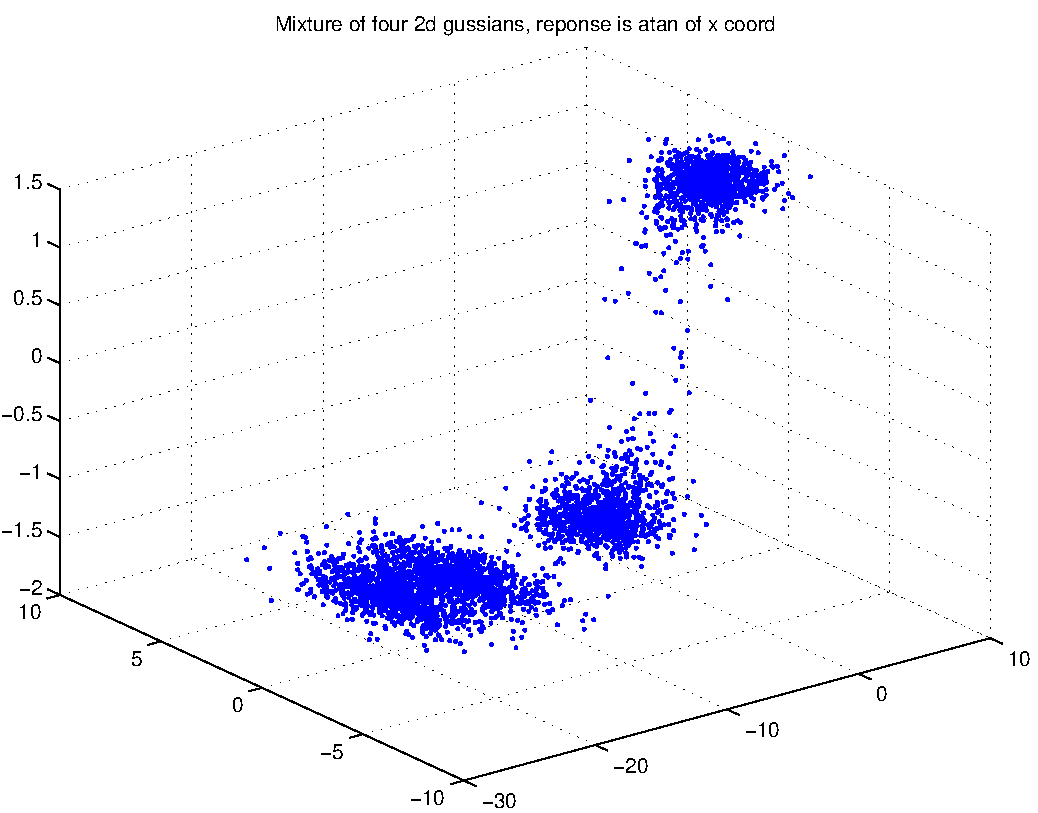
\includegraphics[width=10.0cm,height=10.0cm]{AtanDataSet.pdf}

\subsubsection{3 x 1 Linear Regression}
Sample size = 4000

Number of features = 3

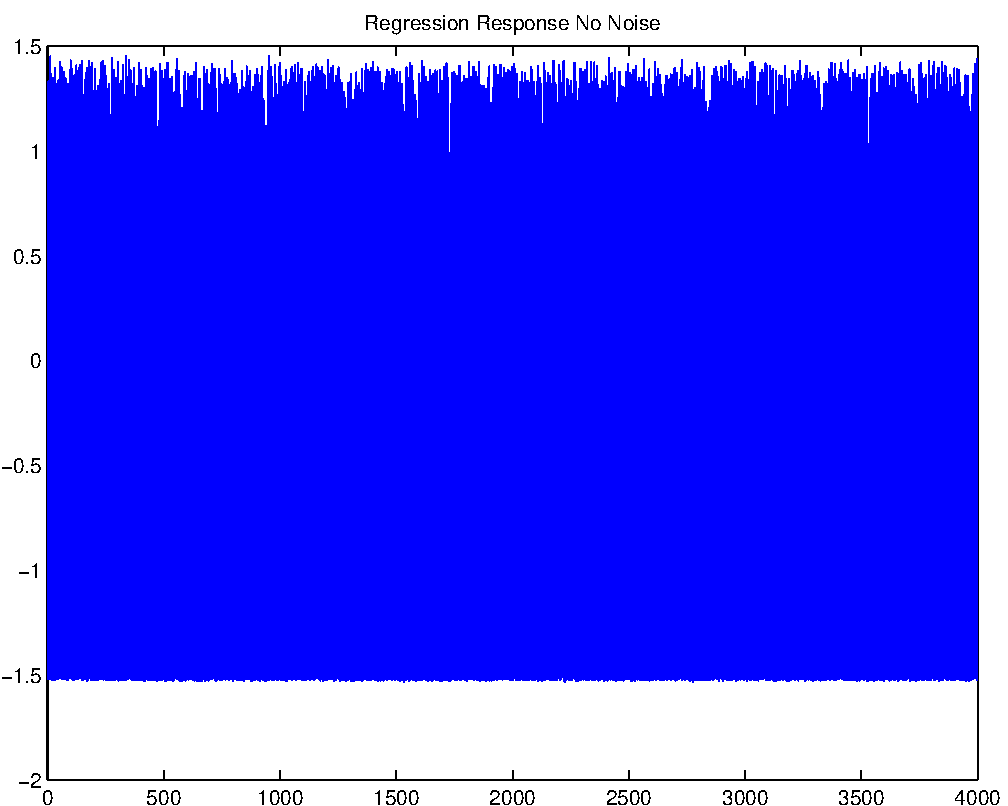
\includegraphics[width=10.0cm,height=10.0cm]{AtanDataSet_regression_response_no_noise.pdf}

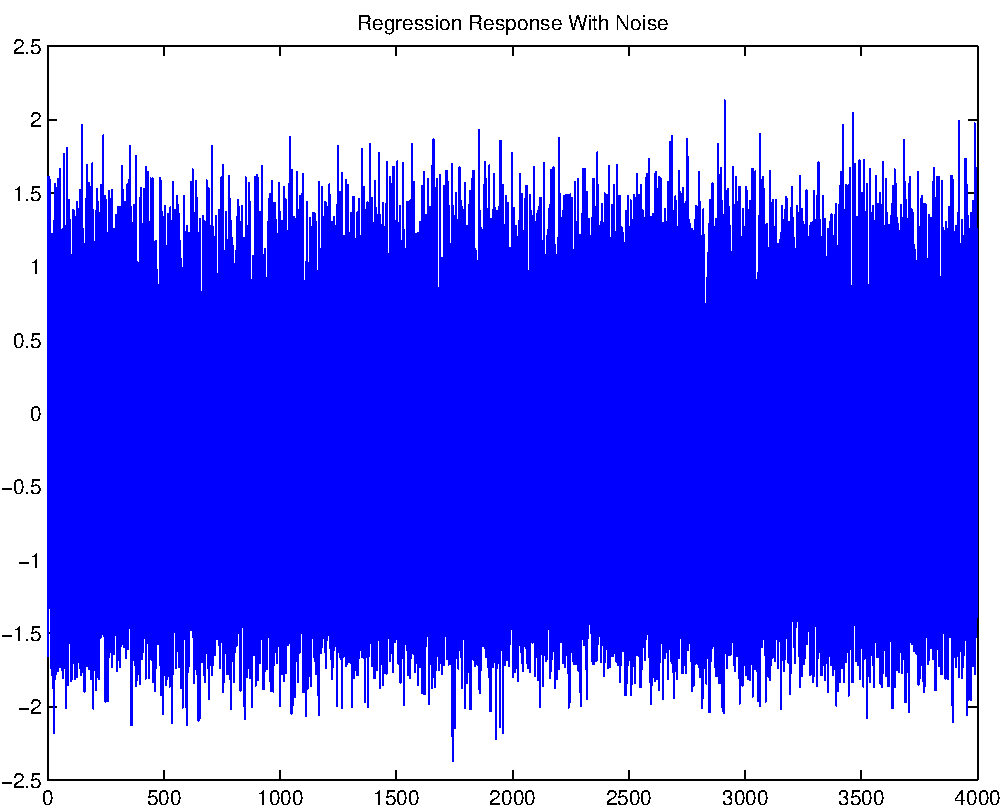
\includegraphics[width=10.0cm,height=10.0cm]{AtanDataSet_regression_response_with_noise.pdf}

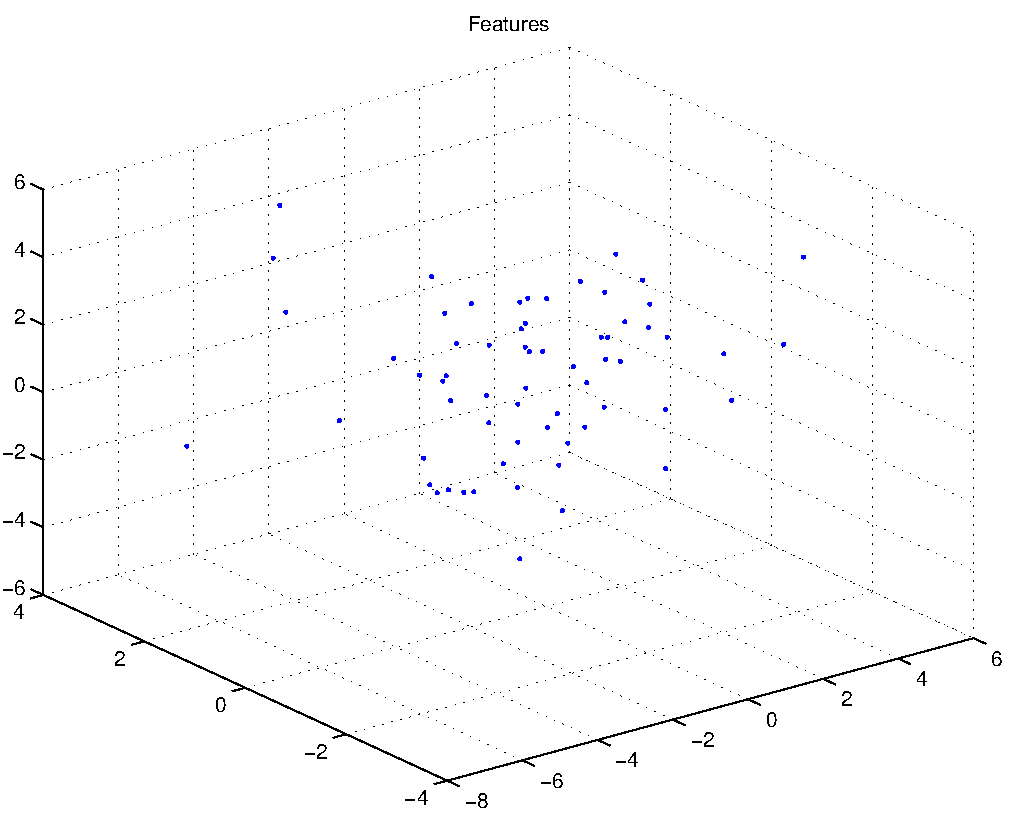
\includegraphics[width=10.0cm,height=10.0cm]{regression_features.pdf}

Response
-1.43687
-1.65575
-1.38349
1.6123
-1.31274
-1.33166
-1.20288
1.57047
-1.29664
-1.09298
0.804151
1.58879
-1.74007
-1.48399
-1.15415
0.952204
-1.17521
-1.36476
-1.78457
1.22304
-1.42609
-1.52062
-1.11813
1.00811
-1.48172
-2.18034
-1.17985
1.31079
-1.45198
-1.7455
-1.15773
1.5633
-1.80927
-1.77973
-1.54404
1.53186
-1.26293
-1.4876
-1.16181
1.03464
-1.16654
-1.36635
-0.822051
1.59555
-1.22994
-1.75868
-1.31393
1.16193
-1.51315
-1.04549
-0.396029
1.66721
-1.55155
-1.73297
-0.962694
1.25076
-1.44974
-1.11086
-1.24539
1.23581
-1.48798
-1.75284
-1.21505
1.25348
-1.80834
-1.28176
-1.29646
1.14087
-1.53264
-1.47344
-0.869387
1.76662
-1.74044
-1.21505
-1.43852
1.02618
-1.60597
-2.008
-0.923411
1.27224
-1.44037
-1.51374
-1.47067
1.80563
-1.34726
-0.99857
-1.46138
1.33595
-1.8521
-1.5456
-1.33129
1.45291
-1.38069
-1.50339
-1.04203
1.31976
-1.37039
-1.19167
0.277929
1.07985
-1.82269
-1.5052
-1.22311
1.07589
-1.69903
-1.81283
-1.15587
1.38688
-1.61434
-1.61536
-1.70222
1.38053
-1.17872
-1.36094
-1.58201
1.22124
-1.81073
-1.39826
-1.60157
1.33612
-1.66459
-1.59513
-1.27059
1.19786
-1.80026
-1.53451
-1.38972
1.44231
-1.41262
-1.22675
-1.46971
1.24552
-1.69591
-1.63842
-1.14157
1.39468
-1.56997
-1.74011
-1.10581
1.51882
-1.66152
-1.4359
-0.850259
1.14931
-1.78658
-1.14797
-0.430742
1.96689
-1.6319
-1.76348
-1.70452
1.25671
-1.48875
-1.7195
-1.43525
1.11768
-1.67816
-1.46964
-1.89972
1.1495
-1.38413
-1.2844
-1.00079
1.46049
-1.67925
-1.56889
-0.918042
1.69413
-1.72283
-1.49488
-1.28012
1.13428
-1.37405
-1.17278
-1.01391
1.28939
-1.62116
-1.7418
-0.203092
1.57028
-1.48596
-1.5625
-1.34805
1.32654
-1.48486
-1.81101
-1.02014
1.53957
-1.54671
-1.41671
-0.876581
1.70221
-1.7348
-1.37304
-1.31914
1.38368
-2.01436
-1.39947
-1.4035
1.162
-1.26507
-1.337
-1.66089
1.16693
-1.35161
-1.39458
-1.89065
1.37626
-1.46668
-1.20922
-1.38597
1.52955
-1.61341
-1.72091
-1.09135
1.44175
-1.51345
-1.79715
-1.56555
1.29797
-1.81493
-1.41695
-1.40273
1.36173
-1.44478
-1.37228
-1.4133
1.32728
-1.52954
-1.06099
-0.48739
1.55831
-1.39054
-1.14923
-1.30048
1.27127
-1.50433
-1.40179
-0.114053
1.894
-1.48056
-1.51783
-1.46815
1.20574
-1.31973
-1.70952
-0.721574
1.47862
-1.9667
-1.50114
-1.25337
1.44993
-1.4364
-1.3519
-0.962684
1.22471
-1.33423
-1.5617
-1.17216
0.868404
-1.96218
-1.46238
-0.793068
1.51568
-1.66572
-1.18313
-1.26607
1.46054
-1.57176
-1.62517
-1.39139
1.40435
-1.61279
-1.39401
0.364243
1.51993
-1.1979
-1.72971
-1.03648
0.961223
-1.34216
-1.43537
-0.71586
1.10847
-1.64305
-1.58573
-1.54207
1.25563
-1.51497
-1.34703
-1.14855
1.0016
-1.43764
-1.28784
-1.34041
1.35082
-1.42245
-1.47135
-1.75821
0.892124
-1.36735
-1.41976
-0.473729
1.40669
-1.68409
-1.60363
-1.15166
0.799907
-1.45603
-1.72908
-1.12436
1.40492
-1.63691
-1.30791
-1.32422
1.2864
-1.58675
-1.49848
-1.24949
1.68258
-1.49839
-1.48937
-1.13792
1.52427
-1.12296
-1.57759
-1.43957
0.97308
-1.41959
-1.5975
-1.47312
1.32214
-1.39656
-1.50539
1.43939
1.32204
-1.42485
-1.20085
-1.66999
1.27007
-1.41966
-1.15864
-1.61118
1.559
-1.13452
-1.60847
-1.43409
1.15137
-1.39598
-1.39242
-0.193958
1.58822
-1.46517
-1.23441
-0.652924
1.82196
-1.60041
-1.46433
-1.22027
1.40836
-2.1272
-1.43332
-1.78272
1.29424
-1.45647
-1.66476
-1.29387
1.21641
-1.61
-1.66275
-0.8699
1.4183
-1.52079
-1.68608
-1.44634
1.26689
-1.58499
-1.71726
-1.68946
1.75041
-1.85806
-1.35762
-1.82129
1.03144
-1.59931
-1.61181
-1.10116
1.0268
-1.23599
-1.32845
-0.452306
0.978195
-1.78136
-1.10169
-1.56224
1.46676
-1.61288
-1.84847
-1.23124
1.53622
-1.11557
-1.6057
-1.43298
0.851515
-1.6742
-1.5339
-1.48723
1.29129
-1.59654
-1.4783
-1.62803
1.26446
-1.50247
-1.43452
-1.43531
1.52901
-1.08243
-1.33312
-1.24536
0.180898
-1.49861
-1.80898
-1.17109
1.67466
-0.95343
-1.56573
-0.816235
1.15486
-1.26224
-1.42331
-1.23411
1.64028
-1.17178
-1.35696
-0.902405
1.30585
-1.80738
-1.68353
-1.38749
1.27277
-1.561
-1.57287
-1.28854
1.59962
-1.25171
-1.3873
-1.68167
1.4461
-1.31691
-1.43198
-0.944575
1.60102
-1.83301
-1.6283
-1.3388
0.878503
-1.15661
-1.22365
-1.186
1.16951
-1.89445
-1.53135
-1.59089
1.1201
-1.25017
-1.74011
-1.6808
1.1762
-1.54174
-1.19248
-1.3168
0.97569
-1.09974
-1.16757
-1.57637
0.787349
-1.39708
-1.10905
-1.42081
0.872383
-1.22641
-1.68725
-1.12315
1.60411
-1.72183
-1.5051
-1.21507
1.58154
-1.92461
-1.43772
-1.29948
1.36834
-1.49856
-1.51066
-1.22175
1.33495
-2.0528
-1.32361
-1.57573
1.26177
-1.22082
-1.25648
-1.37496
1.41019
-1.78773
-1.57456
-1.27774
1.14252
-1.85651
-1.41227
-1.48323
0.345991
-1.81166
-1.58866
-0.511191
1.00709
-1.77482
-1.5156
-1.22813
1.35934
-1.28019
-1.79297
-1.36176
0.939682
-1.86458
-1.7462
-1.62738
1.40333
-1.38566
-1.48397
-1.20401
0.808457
-1.40029
-1.47187
-0.697595
1.30708
-2.11536
-1.32293
-1.24235
1.5773
-1.43475
-1.3032
-1.35956
0.541255
-1.49252
-1.43276
-1.37498
1.38497
-1.46307
-0.932443
-0.948618
1.18751
-1.73584
-1.49784
0.112254
1.47815
-1.62038
-1.37337
-1.19431
1.41634
-1.45269
-1.13666
-1.48023
1.35973
-1.73231
-1.44535
-1.34782
1.17413
-1.0172
-1.54795
-1.53223
1.05172
-1.87306
-1.65989
-1.29931
0.892678
-1.56204
-1.56153
-1.59822
0.901019
-2.00703
-1.33643
-1.03519
0.993887
-1.50325
-1.52068
-1.41201
1.48182
-1.3013
-1.44942
-1.10942
1.11479
-1.4945
-1.58736
-1.41037
1.23552
-1.85472
-2.12472
-1.73319
1.27767
-1.72291
-1.50512
-1.12618
1.1595
-1.7617
-1.29587
-1.16094
1.22521
-1.72368
-1.24115
-1.41568
1.21189
-1.40827
-1.41619
-1.40799
1.57765
-1.22338
-1.48077
-1.21411
1.10015
-1.1817
-1.26236
-0.963316
1.6618
-1.52557
-1.33737
-1.22606
1.22633
-1.31323
-1.83968
-1.42971
1.25211
-1.2913
-1.67665
-1.17187
1.36472
-1.45201
-1.74253
-0.622022
1.58334
-1.77791
-1.26294
-1.0932
1.46801
-1.5262
-1.75537
-1.65223
1.23006
-2.09638
-1.25579
-1.3069
1.22733
-1.1883
-2.07809
-0.992593
1.32304
-1.4385
-1.56513
-1.61648
0.577194
-1.44256
-1.69821
-1.26516
0.824171
-1.11237
-1.28778
-1.62547
1.3458
-1.30756
-1.60161
-1.20437
1.25442
-1.44264
-1.73853
-1.78662
1.30655
-1.82603
-1.83356
-1.66532
1.22378
-1.62676
-1.63851
-1.1338
1.58627
-1.46489
-1.40636
-1.16202
1.53589
-1.73977
-1.47054
-1.17033
1.53331
-1.94724
-1.23398
-1.40552
0.933604
-1.43369
-1.71831
-1.56659
1.10519
-1.39939
-1.54372
-1.44793
1.27301
-1.41259
-1.37013
-0.743814
1.81925
-1.78347
-1.39561
-1.43617
1.27005
-1.71709
-1.36785
-1.58779
1.07276
-1.40072
-1.65015
-0.896377
1.20001
-1.49639
-1.296
-1.05985
1.34273
-1.52124
-1.40926
-1.50435
0.945317
-1.29242
-1.54297
-1.0452
0.766304
-1.52291
-1.40171
-0.918568
1.3871
-1.52855
-1.58168
-1.44118
1.00517
-1.32986
-1.73459
-1.35453
1.36751
-1.27251
-1.55955
-1.31909
1.60715
-1.46175
-1.39438
-1.09892
1.18515
-1.43653
-1.90119
-1.1341
1.69473
-1.52825
-1.8311
-1.30683
0.894642
-1.3266
-1.61616
-1.04159
1.10313
-1.18356
-1.63397
-1.5937
1.3677
-1.54
-1.64417
-1.10785
1.18002
-1.77959
-1.50444
-1.46188
1.17201
-1.74149
-1.41472
-1.56515
1.61978
-1.32511
-1.77929
-1.42978
1.45871
-1.80992
-1.49147
-1.36248
1.31047
-2.01429
-1.44071
-0.416636
1.19274
-1.64349
-1.68872
-0.988675
1.14079
-1.52967
-1.28571
-1.36062
0.726627
-1.41341
-1.7838
-1.83247
1.01427
-1.41187
-1.62818
-1.13629
1.00209
-1.1814
-1.17812
-1.07355
1.10937
-1.58503
-1.56411
-0.785713
1.34048
-1.34006
-1.383
-1.40875
1.45455
-1.08615
-1.49831
-1.37419
1.40563
-1.47503
-1.31213
-1.62957
1.30481
-1.5626
-1.89284
-1.39575
1.27258
-1.17234
-1.44333
-1.13145
1.41299
-1.15253
-1.29569
-1.32468
0.977452
-1.44703
-1.26681
-1.46295
1.19402
-1.99347
-1.32035
-1.4112
0.897744
-2.08616
-1.5686
-1.61795
1.60629
-1.61642
-1.56427
-1.74609
1.1898
-1.79642
-1.40631
-1.08842
1.24068
-1.53166
-1.73762
-1.54095
1.27993
-1.4782
-1.28923
-1.50423
1.56848
-1.65118
-1.80413
-1.20849
1.44165
-1.68025
-1.35269
-1.51613
0.906864
-1.69663
-1.50952
-1.73269
0.594362
-2.00556
-1.13207
-1.33454
1.07349
-1.35094
-1.40515
-1.50742
1.04724
-1.64729
-1.29939
-1.25234
1.60663
-1.57156
-1.19557
-1.8568
1.37288
-1.45687
-1.19344
-1.28222
1.62407
-1.80175
-1.61484
-1.02146
1.60474
-1.81717
-1.78582
-1.13184
1.11137
-1.59909
-1.36424
-1.55649
1.3697
-1.29843
-1.20682
-1.7057
1.17647
-1.54312
-1.4721
-1.49016
1.16339
-1.38652
-0.946961
-1.13131
1.68712
-1.57619
-1.43132
-0.879015
1.07511
-1.88203
-1.70275
-1.83543
0.975866
-1.75853
-1.59458
-1.21149
1.12125
-1.10361
-1.39937
-1.30465
0.919
-0.841594
-1.74384
-1.30944
0.614061
-1.55423
-1.52845
-0.720034
1.30136
-1.49849
-1.4072
0.656564
1.46061
-1.40268
-1.22495
-1.20247
1.49335
-1.82264
-1.65452
-1.01203
1.36531
-1.89435
-1.06751
-1.35258
1.57995
-1.68381
-1.3208
-1.64966
1.43567
-1.69001
-1.38761
-1.89783
0.872182
-1.59795
-1.71975
-1.33181
0.778919
-1.55284
-1.62972
-0.721661
1.4352
-1.27877
-1.43499
-1.37888
1.31634
-1.14276
-1.25784
-1.7002
1.14506
-1.48562
-1.43436
-1.30372
1.22196
-1.3418
-1.36792
-1.39834
1.56678
-1.58969
-1.1644
-0.195591
1.37066
-1.99609
-1.65005
-0.80139
1.13799
-1.61545
-1.59787
-1.15925
1.3119
-1.78047
-1.3249
-1.43231
1.26921
-1.35352
-1.4634
-1.12304
1.53909
-1.8292
-1.45401
-1.43695
1.36356
-1.29068
-1.66146
-0.982622
1.45626
-1.56155
-1.55479
-1.77004
1.09657
-1.5518
-1.46336
-1.45499
0.627107
-1.40035
-1.58225
-1.01032
1.24328
-1.2523
-1.44273
-1.03194
1.56016
-1.51402
-1.4609
-1.3591
1.88525
-1.5717
-1.50497
-1.2311
1.48712
-2.04843
-1.56814
-1.31846
1.65948
-1.44827
-1.99105
-1.57419
1.14053
-1.72419
-1.40459
-1.26383
1.33385
-1.37029
-1.37957
-0.910522
1.32378
-1.93459
-1.31415
-1.05032
1.27289
-1.39746
-1.26043
-1.14178
1.64256
-1.69296
-1.35506
-0.222127
0.886111
-1.83593
-1.50531
-1.14836
1.38153
-1.49433
-1.63636
-1.00045
1.39671
-1.61162
-1.63077
-1.39579
1.47929
-1.38253
-1.43375
-0.800806
1.11034
-1.49681
-1.43514
-1.4139
1.49433
-1.29084
-1.35077
-1.66117
1.63256
-1.90373
-1.33872
-1.21236
0.903062
-1.07996
-1.77045
-1.16919
0.874855
-1.53454
-1.30956
-2.06152
1.031
-1.54583
-1.49332
-1.6436
1.43946
-1.32725
-1.87714
-1.32896
1.02493
-1.54458
-1.27625
-1.37261
0.734002
-1.02884
-1.56365
-0.861515
1.3312
-1.79646
-1.58583
-1.77827
1.15697
-1.49122
-1.85973
-1.14455
1.26555
-1.40664
-1.5354
-1.08879
1.19224
-1.37569
-1.21086
-1.12131
1.36691
-1.66179
-1.24801
-1.36631
0.874797
-1.39274
-1.47656
-1.68967
1.35446
-1.34483
-1.78013
-0.547254
1.30078
-1.64532
-1.28337
-0.765408
0.898863
-1.76087
-1.10342
-1.29786
0.970395
-1.74542
-2.06078
-1.55054
1.57518
-1.59028
-1.53508
-0.977871
1.08386
-1.48264
-1.35637
-1.635
1.11762
-1.17631
-1.57003
-0.785858
1.53931
-1.5964
-1.2059
-0.713884
1.33804
-1.34377
-1.4226
-1.48004
0.806427
-1.53435
-1.26852
-1.09696
1.43832
-1.63092
-1.59277
-1.3929
1.43454
-1.74057
-1.71675
-1.59622
0.836878
-1.36933
-1.46937
-1.54756
1.33661
-1.44124
-1.48887
0.0429115
1.404
-1.51439
-1.45846
-1.40092
1.55989
-1.18124
-1.33339
-1.14195
1.48587
-1.60488
-1.31782
-1.03004
1.21955
-1.6561
-1.8118
-1.2174
1.30012
-1.76515
-1.68783
-0.714287
1.07728
-1.28739
-1.37336
-1.61405
1.33573
-1.462
-1.45255
-1.58806
1.27419
-1.51986
-1.33825
-1.0672
1.11797
-1.1762
-1.28963
-0.969584
1.41629
-1.99922
-1.38341
-1.10313
1.8184
-1.53866
-1.45167
-1.32965
1.01423
-1.62885
-1.60189
-1.47525
1.50825
-1.26492
-1.66431
-1.16774
0.457183
-1.67738
-1.16532
-1.55483
0.820444
-2.00898
-1.48913
-0.97367
1.6376
-1.46319
-1.44604
-0.997631
1.17606
-1.66138
-1.62963
-1.21464
1.20716
-1.59834
-1.6413
-1.35532
1.0565
-1.08616
-1.72272
-1.31159
1.58904
-1.33591
-1.71094
-1.58737
0.149975
-1.49388
-1.33806
-1.55152
1.55467
-1.39338
-1.5389
-1.60764
1.22908
-1.56143
-1.69731
-1.16945
1.12211
-1.53088
-1.29239
-1.36409
1.36409
-1.62102
-1.63868
-1.7069
1.15848
-2.00379
-1.59332
-1.15458
1.26757
-1.51323
-1.26144
-1.3576
1.47389
-1.46306
-1.80599
-1.29449
0.904979
-1.72513
-1.27902
-1.09846
1.02993
-1.7505
-1.20748
-1.22594
1.19136
-1.67519
-1.66586
-1.34544
1.36777
-1.78439
-1.22987
-1.61733
1.02779
-1.57387
-1.47586
-1.21016
1.45643
-1.67231
-1.53762
-1.52416
1.00295
-1.44534
-1.31809
-1.26346
1.20419
-1.26734
-1.22103
-1.10174
1.79983
-1.66194
-1.40146
-1.56736
0.611787
-1.39262
-1.29969
-1.18937
1.53948
-1.52762
-1.67052
-1.04081
1.03384
-1.96581
-1.22849
-1.14187
1.24121
-1.54685
-1.60788
-1.66215
1.3859
-1.54776
-1.22584
-1.18971
1.43719
-2.00169
-1.6822
-1.06548
1.37318
-1.65521
-1.10882
-1.39732
1.39032
-1.55383
-1.33265
-1.48995
1.83716
-1.1833
-1.16846
-1.23866
1.3369
-1.56954
-1.32709
-1.72341
1.46554
-1.34124
-1.60429
-0.0751512
1.11665
-1.21638
-1.41476
-1.27718
1.29461
-1.07018
-1.80859
-1.70632
1.57982
-1.68952
-1.37418
-0.813872
1.39573
-1.38086
-1.1212
-1.45465
1.27379
-1.74781
-1.14844
-1.10888
1.34795
-1.38549
-1.46639
-1.2257
1.77434
-1.32667
-1.5481
-1.34285
1.35268
-1.74176
-1.22807
-1.87191
1.28302
-1.01048
-1.36433
-1.33315
1.22598
-1.70839
-1.53425
-1.02608
1.22605
-1.38433
-1.85281
-1.24544
1.43333
-1.46487
-1.49488
-1.73277
1.26892
-1.77463
-1.72613
-1.29233
1.04361
-1.28839
-1.59588
-1.25707
1.42367
-1.64569
-1.77705
-1.14061
1.70937
-1.72911
-1.52168
-1.11371
0.877594
-1.47997
-1.42919
-1.36015
1.08734
-1.33933
-1.30426
-1.39579
1.6124
-1.64351
-1.69152
-1.36575
1.5614
-1.45713
-1.63338
-0.903168
1.37768
-1.31298
-1.28272
-1.40181
1.33728
-1.76781
-1.41066
-0.97011
1.67989
-1.52313
-1.48155
-1.0575
1.30892
-1.16757
-1.3546
-1.55822
0.969469
-1.29297
-1.54205
-1.33902
1.16796
-1.42365
-1.08328
-1.20349
1.71569
-1.24657
-1.59823
-0.930946
1.29349
-1.70695
-1.27329
-1.27736
1.12123
-1.63404
-1.52045
-1.07182
1.41311
-1.56487
-1.83836
-1.46964
0.915925
-1.16064
-1.36041
-0.985313
1.17387
-1.66493
-1.59847
-1.29676
1.70829
-1.43882
-1.5057
-1.66853
1.24882
-1.98624
-1.37776
-1.30174
-0.465986
-1.5705
-1.18331
-1.48274
1.11647
-1.31963
-1.5373
-0.978495
0.951934
-1.38382
-1.61177
-1.3393
1.44103
-1.78327
-1.34108
-0.97078
1.21463
-1.20256
-1.43454
-1.11875
1.09099
-1.80392
-0.986213
-0.870303
1.45019
-1.59628
-1.59268
-1.66974
1.05519
-1.11066
-1.26646
-0.817088
1.83296
-1.42586
-1.47819
-1.60005
1.38282
-1.58912
-1.63952
-1.50505
1.57462
-1.34749
-1.29634
-1.37829
1.13782
-1.76437
-1.6984
-1.41375
1.22296
-1.69452
-1.7007
-1.57555
0.983294
-1.45682
-1.49456
-1.61533
1.22783
-1.85436
-1.07657
-1.10314
1.08126
-1.62644
-1.24862
-1.72001
1.3025
-1.72937
-1.38091
-1.45585
1.23809
-1.33971
-1.55581
-1.59549
1.0644
-1.27004
-1.90968
0.11828
1.54843
-1.59503
-1.4659
-1.56135
1.08495
-1.17624
-1.4624
-1.044
1.64186
-1.91789
-1.11714
-1.24194
1.23278
-1.63911
-1.45125
-1.44102
1.35118
-1.59076
-1.49128
-1.05811
1.23236
-1.51667
-1.20259
-1.39985
1.59759
-1.37348
-1.35269
-1.22548
1.10308
-1.98547
-1.73951
-1.22086
1.40778
-1.46781
-1.65707
-1.70756
0.882485
-1.53734
-1.58989
-1.14544
1.68699
-1.63427
-1.43817
-1.87684
0.695566
-1.80033
-1.5927
-1.44989
1.86537
-1.40082
-1.39739
-1.59264
1.41653
-1.68905
-1.86798
-0.981482
1.15461
-1.75196
-1.26878
-1.52867
1.53642
-1.29473
-1.59873
-1.1304
1.59743
-1.50941
-1.65412
-1.32775
0.808261
-1.64626
-1.32341
-1.37684
0.853322
-1.75276
-1.48152
-1.18627
1.62543
-1.61614
-1.3528
-1.21404
0.930903
-1.70076
-1.26677
-1.12352
1.05808
-1.72682
-1.77717
-1.59817
0.667289
-1.44893
-1.51239
-1.10748
1.55061
-1.71762
-1.63324
-1.51656
1.21196
-1.13706
-1.37308
-1.38997
1.18103
-1.48937
-1.21033
-0.889061
1.65258
-1.60361
-1.25637
-1.67548
1.33754
-1.29256
-1.34163
-1.10626
1.57875
-1.71402
-1.19267
-1.40582
1.40891
-1.58434
-1.31234
-1.14342
0.596977
-1.70825
-1.67327
-0.996894
1.15258
-1.45252
-1.62696
-1.26932
1.69786
-1.96755
-2.37432
-1.06566
1.41113
-1.79514
-1.99486
-1.36867
1.34409
-1.56035
-1.73119
-1.38611
1.16889
-2.14893
-2.01549
-1.20658
1.49956
-1.56559
-1.48991
-1.19197
1.08217
-1.41469
-1.11534
-1.51232
1.31574
-1.72304
-1.74127
-1.35217
1.09078
-1.37047
-1.61367
-0.958556
1.67519
-1.19079
-1.18955
-1.19089
1.44821
-1.66529
-1.5787
-1.16733
1.34495
-1.8721
-1.61093
-1.68817
1.40623
-1.22581
-1.119
-1.25512
1.38542
-1.53821
-1.44567
-1.38043
1.33416
-1.38377
-1.44574
-1.17096
1.56682
-2.01063
-1.31925
-1.60061
1.19377
-1.68424
-1.48282
-1.36431
1.27591
-1.84122
-1.2602
-1.44652
1.114
-1.37753
-1.76499
-0.150405
1.41687
-1.45326
-1.64624
-1.56696
1.51378
-1.6527
-1.87308
-2.01639
1.41067
-1.57988
-1.36047
-1.46175
1.59297
-1.36393
-1.67386
-1.30629
1.45117
-1.66899
-1.17649
-0.955197
1.65303
-1.68065
-1.62643
-1.38456
1.23774
-1.7246
-0.999636
-1.50452
1.11903
-1.28101
-1.15688
-1.18433
1.10217
-1.69543
-1.7095
-1.35565
0.683738
-1.36075
-1.33183
-1.71365
1.03685
-1.49042
-1.38893
-0.572329
1.9331
-1.88058
-1.53149
-1.08978
1.37679
-1.90921
-1.74707
-1.24137
1.25864
-1.56493
-1.41363
-1.31826
1.15996
-1.29555
-1.43235
-1.58753
1.24567
-1.36902
-1.24534
-1.13179
1.55355
-1.52458
-1.46691
-1.18329
1.71333
-1.60257
-1.44411
-1.55945
1.59764
-1.54885
-1.37352
-1.66095
0.545251
-1.51079
-1.11013
-1.22612
1.08251
-1.46901
-1.73198
-1.10465
1.39584
-1.10719
-1.79559
-1.02214
1.68824
-1.24693
-1.74162
-1.70779
0.737243
-2.03331
-1.58364
-1.38227
1.32197
-1.64572
-1.35081
-1.38288
0.76405
-1.39102
-1.64501
-1.7332
1.3859
-1.62927
-1.64854
-0.976029
1.63004
-1.36397
-1.69559
-1.26325
1.39804
-1.39315
-1.68912
-1.44189
1.3458
-2.22297
-1.1581
-1.35375
1.37893
-1.73593
-1.40101
-1.4639
1.02728
-1.37734
-1.28088
-1.55112
1.40352
-1.70444
-1.61748
-1.42217
1.36263
-2.14012
-1.44786
-0.723953
1.85597
-1.33621
-1.26491
-1.08958
1.69165
-1.39836
-1.61557
-1.17996
1.42183
-2.18298
-1.82889
-1.47643
1.55511
-1.28208
-1.1475
-1.6399
1.27996
-1.2518
-1.71597
-1.51655
1.17564
-1.27814
-1.30166
-0.829524
1.48099
-1.52096
-1.31528
-1.18459
1.31701
-1.68397
-1.38047
-1.1992
1.42948
-0.956862
-1.59267
-1.04818
1.1016
-1.43141
-1.72311
-1.56796
1.12744
-1.50764
-1.40527
-1.18243
0.911002
-1.3147
-1.30994
-0.985832
1.77505
-1.4729
-1.45168
-1.06372
1.04147
-1.29215
-1.80164
-1.60302
1.23745
-0.808091
-1.47915
-0.167875
1.3992
-1.76602
-1.3503
-1.13197
1.23992
-1.15178
-1.32992
-1.29131
1.27804
-1.73591
-1.3173
-1.01627
1.20467
-1.6678
-1.82881
-1.305
1.13769
-1.55026
-1.48007
-1.40502
1.30675
-1.29293
-1.5778
-1.25935
1.62695
-1.58352
-1.42725
-1.20837
1.26488
-1.55193
-1.62857
-1.0643
1.49547
-1.45532
-1.70571
-1.43704
1.15612
-1.75768
-1.2842
-1.07518
1.23844
-1.43248
-1.43397
-1.33775
1.46267
-1.31093
-1.58785
-1.27299
1.26855
-1.45288
-1.60336
-1.47678
1.54942
-1.70182
-1.06323
-1.20479
0.968829
-1.43446
-1.73635
-1.61187
0.917493
-1.50513
-1.36404
-1.38413
0.830036
-1.43032
-1.76504
-1.50999
1.48858
-1.53299
-1.33888
-1.28856
1.38018
-1.54445
-1.33131
-0.95343
1.34491
-1.51684
-1.56458
-1.55106
1.28814
-1.40778
-1.4243
-1.18977
1.67474
-1.30701
-1.25754
-1.22199
0.747481
-1.78357
-1.79292
-1.21815
1.30305
-1.3671
-1.58515
-1.12471
1.35532
-1.35801
-1.66016
-1.03239
1.37606
-1.50889
-1.82234
-1.70606
1.40727
-1.62926
-1.66137
-1.27646
1.06557
-2.00159
-1.29438
-1.51225
1.46586
-1.58307
-1.41002
-1.56785
1.31871
-1.28675
-1.64248
-1.21674
1.1159
-1.31279
-1.86308
-0.894497
1.17355
-1.31455
-1.43215
-0.44559
1.70419
-1.46453
-1.47703
-1.03077
1.07652
-1.64987
-1.51913
-0.954722
0.715697
-1.68884
-1.40914
-1.34426
1.20897
-1.67646
-1.39621
-1.46413
1.25023
-1.4366
-1.44426
-1.08551
1.3924
-1.39829
-1.4723
-0.918057
1.41688
-1.53506
-1.80588
-1.28277
1.65625
-1.75826
-1.09622
-1.10088
1.1191
-1.67342
-1.35147
-1.04758
1.5237
-1.20556
-1.62246
-0.381668
1.67561
-1.51902
-1.41858
-1.46626
1.30659
-1.87415
-1.56573
-1.22679
1.1436
-1.39553
-1.54218
-1.42918
1.07743
-1.47693
-1.48913
-1.56489
1.03295
-1.81446
-1.65761
-1.27867
1.19052
-1.17976
-1.74641
-0.646338
1.8764
-1.74493
-1.43184
-1.36302
1.49382
-1.42144
-1.38301
-1.25852
1.17816
-1.56205
-1.53301
-0.955926
1.32866
-1.21163
-1.04095
-0.611444
1.37453
-1.48537
-1.70584
-0.342908
1.48187
-1.36857
-1.67986
-1.03154
0.738188
-1.73362
-1.61461
-1.38786
-0.584048
-1.42356
-1.0029
-1.47229
1.48857
-1.64698
-1.44366
-0.910312
1.10883
-1.67476
-1.77176
-1.08597
1.23622
-2.00695
-1.6582
-1.20473
1.48439
-1.33885
-1.97005
-1.20769
1.49089
-1.29977
-1.29873
-1.07869
1.34805
-1.53013
-1.45662
-1.10932
1.4633
-1.6334
-1.34659
-1.20364
1.10949
-1.61884
-1.69008
-0.906556
1.06426
-1.46158
-1.71247
-0.81356
1.57615
-1.54624
-1.51478
-1.09069
1.3049
-1.65414
-1.71066
-1.48816
1.22325
-1.49911
-1.396
-1.36956
1.59703
-1.72941
-1.75486
-1.68422
0.734495
-1.64049
-1.31063
-1.42438
1.21731
-1.90091
-1.35152
-1.32343
1.0917
-1.99553
-1.41341
-1.39269
1.21808
-1.54265
-1.48054
-1.34846
1.35955
-1.44001
-1.50992
-1.01937
1.66645
-1.24792
-1.24194
-1.58031
1.58006
-1.47953
-1.36704
-1.43701
1.66234
-1.33894
-1.7435
-1.36833
1.23146
-1.50768
-1.28503
-0.261938
1.5085
-1.48205
-1.95077
-1.01938
1.2736
-1.5212
-1.37036
-1.39131
1.32042
-1.43182
-1.43668
-1.40681
1.20573
-1.39655
-1.395
-0.765658
1.15123
-1.4997
-1.25379
-1.24144
1.11932
-1.48541
-1.68971
-1.27589
1.33252
-1.60128
-1.7117
-1.35701
1.59539
-1.30831
-1.7073
-0.507937
1.58261
-1.69003
-1.53742
-1.27371
1.40668
-1.55089
-1.38725
-1.5875
1.19202
-1.68879
-1.13611
-0.870451
1.77712
-1.38858
-1.57842
-1.00414
1.55219
-1.53293
-1.29287
-1.49228
1.2769
-1.496
-1.5218
-1.11744
1.24197
-1.43502
-1.38125
-1.69821
1.30042
-1.35245
-1.48356
-1.33867
1.42569
-1.37999
-1.49553
-1.39052
1.17444
-1.58066
-1.41605
-1.3744
1.29408
-1.79233
-1.52754
-1.43987
1.49741
-1.2919
-1.53436
-1.69478
1.18542
-1.4266
-1.54827
-1.33056
1.48888
-1.60563
-1.45116
-1.05084
0.944865
-1.31432
-1.66016
-1.73822
1.43987
-1.32317
-1.08469
0.833508
1.68495
-1.3437
-1.73167
-1.10913
1.19606
-1.45567
-1.11735
-1.47209
0.989226
-1.47909
-1.4885
-1.00715
1.4163
-1.46332
-1.65487
-1.05195
1.28184
-1.48411
-1.08185
-1.32475
1.55201
-1.40318
-1.53648
-0.947948
1.23198
-1.49591
-1.63728
-0.894981
0.869247
-1.58399
-1.69389
-1.26361
1.69178
-1.29614
-1.57628
-1.50979
1.40799
-1.71662
-1.59894
-1.59269
1.2321
-1.46047
-1.33087
-1.36517
1.48198
-1.53373
-1.82976
-1.41576
1.26936
-1.71771
-1.66551
-1.21905
1.13859
-1.29035
-1.62314
-1.01906
1.2617
-1.44103
-1.44308
-1.61926
1.22574
-1.57829
-1.22947
-1.42382
1.16014
-1.60197
-1.4525
-1.51403
1.137
-1.26223
-1.92141
-1.25166
1.37773
-1.55435
-1.84284
-1.44431
1.17035
-1.66353
-1.3941
-0.938206
1.47751
-1.7176
-1.51997
-0.917462
1.26699
-0.96939
-1.6841
-1.44303
0.788906
-1.56467
-0.968084
-1.21222
1.44961
-1.71961
-1.69022
-1.91988
1.31805
-1.70112
-1.84737
-1.64538
0.958821
-1.07771
-1.24025
-0.768789
1.3153
-1.72101
-1.70499
-1.06212
1.48812
-1.63486
-1.81
-1.84011
0.505421
-1.46195
-1.44125
-0.711118
1.46675
-1.44196
-1.65101
-1.50243
1.63032
-1.29121
-1.17932
-1.38506
1.0447
-1.31735
-1.30404
-1.23134
1.48435
-1.54847
-1.65858
-1.20351
1.26631
-1.24907
-1.86644
-1.0315
1.55663
-1.55317
-1.44863
-1.74871
0.878259
-1.02605
-1.06678
-1.44145
1.38155
-1.59744
-1.52497
0.651933
1.23975
-1.26659
-1.31734
-1.24274
1.30884
-1.68183
-1.29885
-1.40858
1.32953
-1.30849
-1.26996
-1.53987
1.60386
-1.38653
-1.21612
-1.31086
1.63305
-1.46806
-1.41765
-1.5079
0.957503
-1.66286
-1.44129
-1.06988
1.73273
-1.49312
-1.44082
-1.57762
0.843128
-1.83187
-1.69695
-1.98377
1.33849
-1.66098
-1.85507
-1.36889
1.25138
-1.67973
-1.6521
-1.25605
1.36047
-0.982835
-1.79923
-1.66762
0.971123
-1.08659
-1.74316
-0.153086
1.63152
-1.82824
-1.47893
-1.26717
1.64253
-1.28105
-1.1403
-1.42644
1.37856
-1.81203
-1.64821
-0.933504
1.52516
-1.46748
-1.18022
-0.867203
1.60979
-1.88627
-1.45247
-1.23131
1.43583
-1.25549
-1.69828
-1.58428
1.60589
-1.49462
-1.36694
-1.56878
1.59403
-1.44238
-1.5027
-1.11154
1.06274
-1.25633
-1.94691
-1.28963
1.29636
-1.40847
-1.44721
-1.51354
1.13844
-1.57845
-1.67241
-1.18208
1.38947
-1.45197
-1.31385
-1.32473
1.28889
-1.39559
-1.46623
-1.62576
1.30088
-1.17803
-1.52783
-1.3137
1.57775
-1.81333
-1.58441
-1.35903
1.50806
-1.60926
-1.59386
-1.33118
1.85082
-1.21195
-1.58399
-1.36877
1.6829
-1.17363
-1.68718
-1.22319
1.88987
-1.57563
-1.7015
-1.186
1.3775
-1.67333
-1.76623
-1.42798
0.916175
-1.42645
-1.94291
-0.940672
1.10817
-1.62845
-1.59118
-1.51892
1.47671
-1.73405
-1.75598
-1.35461
1.44701
-1.59996
-1.81521
-1.18209
1.26857
-1.40764
-1.38456
-1.31141
1.03986
-1.65154
-1.67228
-1.39018
1.6485
-1.14402
-1.06336
-1.34824
1.50812
-1.50983
-1.19724
-1.03591
1.01681
-1.3962
-1.53337
0.228036
1.49621
-1.53845
-1.58196
-1.77454
1.53596
-1.74274
-1.17629
-1.36664
1.00356
-1.51132
-1.34792
-1.041
1.42765
-1.44016
-1.35159
-1.72022
1.27503
-1.56027
-1.77285
-1.30764
1.44239
-1.359
-1.19683
-1.04397
1.86972
-1.46118
-1.61618
-0.964028
1.74636
-0.994601
-1.38162
-1.30216
1.31416
-1.56558
-1.51897
-1.07982
1.29006
-1.56223
-1.38124
-1.55019
0.787755
-1.40711
-1.89392
-1.6835
1.25203
-1.62794
-1.36192
-0.912457
1.24071
-1.61022
-1.2947
-1.85668
-0.570145
-1.68983
-1.77995
-1.62799
1.31802
-1.37179
-1.28642
-1.08501
1.41248
-1.68865
-1.43279
-0.75467
1.28866
-1.7039
-1.1147
-1.46707
1.40195
-1.71262
-1.43463
-1.0385
1.64668
-1.47199
-1.73113
-1.34176
0.964395
-1.80115
-1.52861
-1.34106
1.44027
-1.11394
-1.51607
-1.4739
1.2003
-2.01322
-1.3459
-1.38403
1.2115
-1.77167
-1.94233
-1.2824
1.38838
-1.46454
-1.31475
-1.24192
1.21514
-1.73918
-0.932041
-1.18872
0.741002
-1.48071
-1.42111
-1.22573
0.631756
-1.8432
-1.55018
-1.67178
0.922628
-1.56347
-1.36513
-1.22166
1.09407
-1.28561
-1.65269
-1.58009
1.29122
-1.85417
-1.22599
-2.03782
1.45368
-1.23543
-1.74946
-1.63378
1.27999
-1.69028
-1.43735
-0.967179
1.19085
-1.60401
-1.07222
-1.22677
1.56727
-1.59165
-1.2249
-0.910018
0.964358
-1.30165
-1.21516
-1.37712
1.19494
-1.7292
-1.5875
-1.5253
1.26872
-1.65947
-1.28067
-1.0509
1.32526
-1.79451
-1.12365
-1.09315
1.20201
-1.0868
-1.62866
-1.71002
1.83484
-1.34892
-1.29143
-1.29848
1.62295
-1.36613
-1.84176
-1.71371
0.586637
-1.19633
-1.4603
-1.19203
1.67184
-1.56557
-1.42287
-1.3225
1.44338
-2.00402
-1.32915
-0.981562
1.35048
-1.44748
-1.67265
-2.03046
0.532304
-2.045
-1.43211
-1.2518
2.13112
-1.60541
-1.15247
-1.02939
1.51359
-1.54785
-1.634
-1.0485
0.891747
-1.73601
-1.66968
-1.00443
1.27711
-1.19434
-1.54603
-1.50814
1.52612
-1.64922
-1.33721
-0.130235
1.40374
-1.63087
-1.34544
-1.33991
1.27501
-1.48123
-1.64585
-0.580771
1.09578
-1.28834
-1.50238
-1.34333
1.08294
-1.27802
-1.55998
-1.12221
1.67993
-1.08983
-1.34016
-0.90141
1.41845
-1.71611
-1.48145
-1.39003
1.33122
-1.49845
-1.75757
-1.008
1.60717
-1.44446
-1.27473
-1.6549
1.11762
-0.933565
-1.56735
-1.35619
1.40836
-1.48097
-1.15598
-0.930385
1.43851
-1.64885
-1.80365
-1.5172
1.5445
-1.98011
-1.68486
-1.39293
1.50892
-1.63326
-1.64688
-1.43105
1.19779
-1.74755
-1.77171
-1.1399
0.910311
-1.85804
-1.07683
-1.43555
1.39076
-1.61342
-1.34551
-1.68703
1.24508
-1.23334
-1.40137
-1.40142
1.2665
-1.45724
-1.72008
-1.37469
1.54157
-1.78613
-1.27251
-0.863348
1.51519
-1.65835
-1.5695
-1.10202
1.38252
-1.40406
-1.73598
-1.81304
1.23302
-1.6053
-1.18326
-0.695437
1.44921
-1.50797
-1.81692
-1.58367
1.36461
-1.60821
-1.71256
-1.43629
1.25416
-1.46014
-1.24792
-0.435258
1.66644
-1.93224
-1.62383
-0.689252
0.800476
-1.57062
-1.55039
-0.942554
0.907334
-1.60739
-1.74491
-0.867268
1.64763
-1.59145
-1.5852
-1.71082
0.905409
-1.52117
-1.75939
-1.19029
0.787215
-1.55765
-1.56221
-0.878182
0.956616
-1.96284
-1.79655
-1.5711
1.34635
-1.80423
-1.53482
-0.897078
1.90426
-1.99796
-1.39437
-1.5839
1.58735
-1.50304
-1.52036
-0.91255
1.29847
-1.59369
-1.35545
-1.25263
1.61147
-1.27625
-1.54066
-1.04784
1.52636
-1.3534
-1.46719
-1.26752
1.2808
-1.64835
-0.948357
-0.655047
1.27275
-1.96609
-1.19612
-0.979003
1.17897
-1.56813
-1.24263
-0.9238
1.29219
-1.50759
-1.33681
-1.07755
0.938738
-1.79621
-1.5118
-0.575489
1.12545
-1.78081
-1.3955
-1.01473
1.64996
-1.82411
-1.59383
-1.47741
0.905063
-1.51949
-1.52463
-1.19559
1.43507
-1.63939
-1.66798
-1.16853
1.45091
-1.21482
-1.40142
-1.50426
1.26729
-1.57874
-1.36823
-1.68928
1.06279
-1.391
-0.937474
-1.13887
1.4552
-1.24915
-1.07482
-1.53638
0.651209
-1.5181
-1.50894
-1.39637
1.15578
-1.7398
-1.71256
-1.38184
0.988645
-1.44643
-1.39208
-1.10971
0.960311
-1.53805
-1.55491
-1.54969
1.18112
-1.52249
-2.01894
-1.15611
1.22784
-1.63908
-1.62521
-1.31932
1.41418
-1.20001
-1.40431
-1.59238
1.31588
-1.58626
-1.75972
-1.64831
0.990902
-1.57917
-1.52962
-0.853677
1.38609
-1.67734
-1.41637
-1.16782
1.47548
-1.53101
-1.5243
-1.46128
1.4616
-1.40622
-1.19908
-1.4466
0.753155
-1.2373
-1.69995
-1.0109
1.30156
-1.60618
-1.26321
-1.62251
1.09787
-1.91458
-1.87668
-1.52332
1.39675
-1.77303
-1.7498
-1.28851
1.54281
-1.25017
-1.37815
-0.996041
1.33211
-1.32659
-1.41559
-1.09788
1.30096
-1.49803
-1.59582
-1.18242
1.19559
-1.64257
-1.58394
-1.70432
0.92546
-1.05531
-1.44201
-1.46108
1.11658
-1.2455
-1.32694
-1.13594
1.41225
-1.23196
-1.33555
-1.10145
1.33463
-1.42009
-1.23814
-1.65735
1.36416
-1.55117
-1.42634
-0.124848
1.61372
-1.86889
-1.63872
-0.911589
1.06841
-1.64643
-1.7417
-1.38107
1.38995
-1.79521
-1.50997
-1.71466
1.30671
-1.57079
-1.67859
-1.23461
1.28174
-1.71214
-1.5876
-1.21891
1.15684
-1.67032
-1.35793
-1.32024
1.04082
-1.49838
-1.49041
-0.874913
1.51795
-1.57606
-1.10683
-1.40227
1.44979
-1.47473
-1.10795
-1.32173
1.13822
-1.40803
-1.48314
-1.46321
1.20369
-1.40137
-1.61318
-0.924267
1.27243
-1.7874
-1.72772
-1.52188
1.2956
-1.77559
-1.27139
-1.51661
1.25402
-1.23719
-1.47324
-1.0697
1.29977
-1.8327
-1.356
-1.34816
1.51166
-1.79225
-1.24116
-0.985712
1.31729
-1.341
-1.41286
-1.3706
1.14608
-1.43686
-1.29587
-1.45506
1.47704
-1.50783
-1.8602
-1.21901
1.43983
-1.10665
-1.66794
-1.33132
1.70926
-1.04048
-1.15199
-1.51278
1.05587
-1.62835
-1.36508
-1.42912
1.31929
-1.17418
-1.40979
-1.42821
0.693001
-1.78687
-1.51472
-1.19247
1.20145
-1.52765
-1.66178
-1.20635
1.47679
-1.26346
-1.71825
-1.59339
1.19612
-1.53254
-1.7443
-1.11654
1.32025
-1.822
-1.57888
-0.984779
1.06345
-1.4809
-1.60542
-0.992633
1.01288
-1.70422
-1.51068
-1.50213
1.25293
-1.90183
-1.58803
-1.14731
1.06207
-1.59877
-1.12989
-1.19499
1.30308
-1.49159
-1.34977
-1.65633
1.34437
-1.43
-1.71483
-0.926707
1.35502
-1.51141
-1.34642
-1.26215
0.996357
-1.54352
-1.7837
-1.0198
1.20571
-1.65175
-1.74357
-1.14834
0.767488
-1.17647
-1.19836
-0.853417
1.35009
-1.70613
-1.77519
-1.34589
1.42596
-1.99386
-1.34461
-1.60626
0.881308
-1.67724
-1.12175
-1.61939
1.1385
-1.89442
-1.13315
-1.12558
1.4163
-1.63759
-1.34259
-1.11983
1.54809
-1.83206
-1.44109
-0.854114
1.64428
-1.56209
-1.46521
-1.14783
1.36508
-1.31023
-1.73689
-0.699035
1.96347
-1.0466
-1.50157
-0.884015
1.38306
-1.83273
-1.16477
-1.22997
1.3284
-1.32824
-1.15025
-1.35926
1.21652
-1.69646
-1.51102
-1.09779
1.5579
-1.63054
-1.44146
-1.37987
1.14865
-1.42686
-1.24365
-0.185233
1.55226
-1.26638
-1.92519
-1.02708
1.26346
-1.27077
-1.60892
-1.02749
1.67338
-1.53533
-1.30722
-1.25567
0.734469
-1.36356
-1.32218
-1.48904
0.869207
-1.57764
-1.83541
-1.03712
2.04832
-1.54804
-1.46024
-1.18777
1.3098
-1.30369
-1.21691
-1.24394
1.70131
-1.42767
-1.44358
-1.4282
1.1602
-1.69015
-1.3451
-1.13772
1.33759
-1.66513
-1.59146
-1.47536
0.906408
-1.71367
-1.54744
-1.28337
1.32592
-1.61133
-1.50675
-1.15231
1.72325
-1.31918
-1.81546
-1.19579
0.754347
-1.3837
-1.42326
-1.24691
1.17893
-1.31604
-1.60293
-1.29162
1.5034
-1.17991
-1.65519
-1.14445
1.21557
-1.86479
-1.31428
-1.12867
1.72705
-1.6785
-1.66425
-1.628
0.944428
-1.45149
-1.35921
-1.26467
1.37196
-1.09606
-1.55446
-0.986062
1.56251
-1.35214
-2.07898
-1.42558
0.872438
-1.4552
-1.50197
-1.5258
0.777759
-1.63766
-1.18809
-1.36716
1.66607
-1.83129
-1.29778
-1.24453
1.36661
-1.32231
-1.65181
-1.28164
1.35484
-1.36952
-1.20625
-1.14194
1.17075
-1.71989
-1.54549
-1.42162
1.41231
-1.44114
-1.8692
-1.09178
0.852253
-1.48671
-1.22655
-0.93306
1.30727
-1.17038
-1.46652
-1.28087
1.61854
-1.43274
-1.66401
-1.33149
1.21673
-1.47066
-1.41198
-1.65996
1.4249
-1.64648
-1.32681
-1.36238
1.3911
-1.61502
-1.54533
-0.996945
1.50068
-1.3198
-1.8435
-1.43456
1.30755
-1.61618
-1.64789
-1.63136
1.41789
-1.8662
-1.42854
-1.39703
1.7147
-1.77069
-1.58078
-1.52639
1.27815
-1.29222
-1.05864
-1.61767
1.0127
-1.59416
-1.26642
-1.1299
0.870424
-1.79321
-1.20178
-1.0689
1.59567
-1.3935
-1.62933
-1.43602
1.36416
-1.65834
-1.0446
-0.687962
1.25061
-1.86245
-1.30132
-1.23852
1.27992
-1.45861
-1.55771
-1.37621
0.971177
-1.42356
-1.16158
-1.09081
1.34043
-1.07505
-1.34998
-1.36774
1.4287
-1.63847
-2.00947
-0.937314
1.54879
-1.67293
-1.79198
-1.19053
1.22872
-1.64246
-1.59744
-1.6731
1.66075
-1.86453
-1.54824
-1.65688
1.56039
-1.35108
-1.60201
-1.07763
1.32868
-1.75418
-1.68671
-1.11519
1.29009
-1.73537
-1.6873
-1.47816
1.24378
-1.13506
-1.76798
-1.6403
1.04418
-1.30704
-1.41268
-1.01004
1.21124
-1.41361
-1.4422
-1.40133
1.42187
-1.61572
-1.77477
-1.04579
1.27379
-1.67674
-1.6583
-1.5242
1.33046
-1.46043
-1.49247
-1.23826
1.86342
-0.960575
-1.60592
-1.27122
1.57428
-1.24707
-1.97
-1.02268
1.45133
-1.55125
-1.31307
-1.39311
1.32312
-1.56827
-1.68908
-1.28515
1.10828
-1.64023
-1.7666
-0.872034
1.56278
-2.03966
-1.38525
-1.07292
1.60889
-1.20189
-1.55942
-1.1642
0.532046
-1.18414
-1.12756
-1.49287
1.38933
-1.57712
-1.4511
-1.52861
1.36624
-1.44109
-1.27768
-1.32817
1.27147
-1.38188
-1.41689
-0.962444
1.14416
-1.62259
-1.48775
-0.968078
1.11054
-1.51735
-1.24087
-1.39546
0.854537
-1.63913
-1.35472
-1.41267
1.03456
-1.57882
-1.27878
-1.14562
1.6414
-1.63094
-1.85192
-0.996913
1.15151
-1.84268
-1.80336
-1.52417
1.27163
-1.43106
-1.55452
-0.985712
1.45808
-1.3719
-1.6061
-1.10301
1.48252
-1.43208
-1.72046
-1.17546
1.1863
-1.8251
-1.07028
-1.21126
1.2692
-1.67441
-1.903
-1.61482
1.42773
-1.85957
-1.74094
-1.19867
1.1741
-1.40708
-1.21052
-1.48034
1.42084
-1.26667
-1.52834
-1.23555
1.05175
-1.51381
-1.71195
-1.2782
0.863682
-1.41995
-1.27495
-0.0971476
1.3539
-1.68011
-1.34408
-1.39139
1.22574
-1.43957
-1.6037
-1.22561
1.32766
-1.58889
-1.45881
-1.48528
1.19418
-1.57905
-1.43679
-1.06319
1.57517
-1.67881
-1.5535
-0.406248
1.67155
-1.63633
-1.54532
-1.24799
1.46771
-1.65209
-1.53892
-1.88754
1.33801
-1.80283
-1.63614
-1.47635
1.61158
-1.41225
-1.50741
-0.881467
1.44355
-1.60903
-1.51572
-0.987592
1.61019
-1.18453
-1.71465
-1.72688
0.755218
-1.58096
-1.64428
-1.43137
0.929263
-1.11605
-1.76012
-1.19389
0.915804
-1.7781
-1.35244
-0.535522
1.58183
-0.694799
-1.41471
-1.4977
1.26079
-1.46779
-1.44475
-0.983746
1.02199
-1.39852
-1.38355
-0.977771
1.24388
-1.56798
-1.81144
-1.32078
1.30134
-1.7207
-1.70917
-1.2752
1.09895
-1.11209
-1.20652
-1.05006
1.25714
-1.44485
-1.8119
-1.42833
1.4041
-1.32275
-1.50627
-1.07743
0.916211
-1.13779
-1.52854
-1.45042
1.57917
-1.38263
-1.35727
-1.25805
1.61677
-1.98907
-1.49229
-1.54909
1.59253
-2.10398
-1.41441
-1.59264
1.12008
-1.3697
-1.66223
-1.1947
1.1938
-1.19147
-1.31025
-1.12905
1.23239
-1.14227
-1.41195
-1.72831
1.273
-1.38419
-1.50281
-1.15899
0.798089
-1.65706
-1.46002
-1.0177
1.36527
-1.32254
-1.18454
-1.30933
1.99183
-1.79637
-1.66828
-0.995727
1.15464
-1.59542
-1.39042
-1.62131
1.08312
-1.58194
-1.50116
-1.57535
1.31803
-1.80581
-1.75309
-1.14167
1.17427
-0.589121
-1.66842
-1.73096
1.20446
-1.6489
-1.12024
-1.62622
1.15003
-1.30617
-1.51204
-1.13434
1.73278
-1.5461
-1.20907
-1.5389
0.907571
-1.78324
-2.06005
-1.22097
1.55636
-1.35659
-1.80766
-1.7002
1.34488
-1.95257
-1.56042
-1.21632
1.25346
-1.32922
-1.89247
-1.20382
0.19202
-1.63868
-1.80098
-1.95668
1.36165
-1.5254
-1.56737
-1.64261
1.23639
-1.70655
-1.19567
-1.25804
1.44601
-1.72262
-1.3587
-1.32884
1.36488
-1.58242
-1.60421
-0.279258
1.97472
-1.65437
-1.77785
-0.946302
1.6693
-1.41126
-1.52884
0.198092
1.04135
-1.08062
-1.39281
-1.21884
1.25925
Estimate for Beta
0.000299912
-0.000395098
0.996784
QueryPerformanceCounter  =  5.3626
\subsubsection{Linear Regression 3x1}
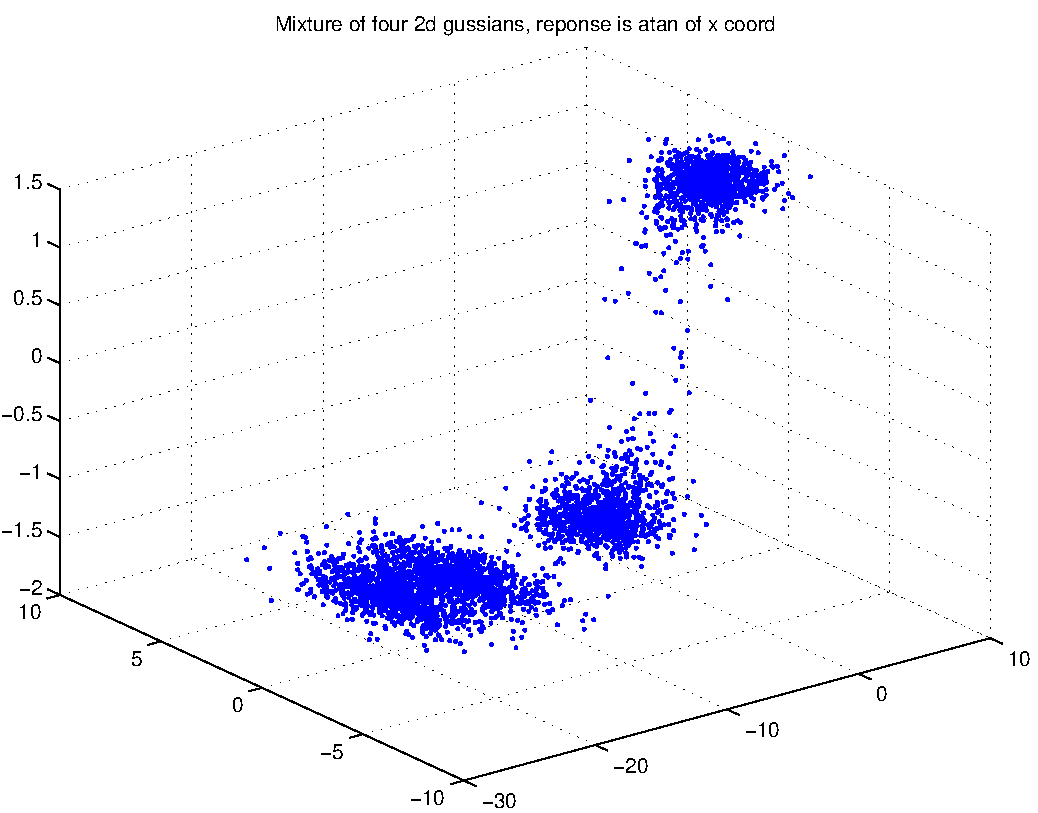
\includegraphics[width=10.0cm,height=10.0cm]{AtanDataSet.pdf}

\subsubsection{3 x 1 Linear Regression}
Sample size = 64

Number of features = 3

$\sigma = \left(
\begin{array}{
ccc}
+3.952 & -0.499 & -0.010 \\
-0.499 & +1.895 & +0.465 \\
-0.010 & +0.465 & +4.477 \\
\end{array}
\right)$ \newline 

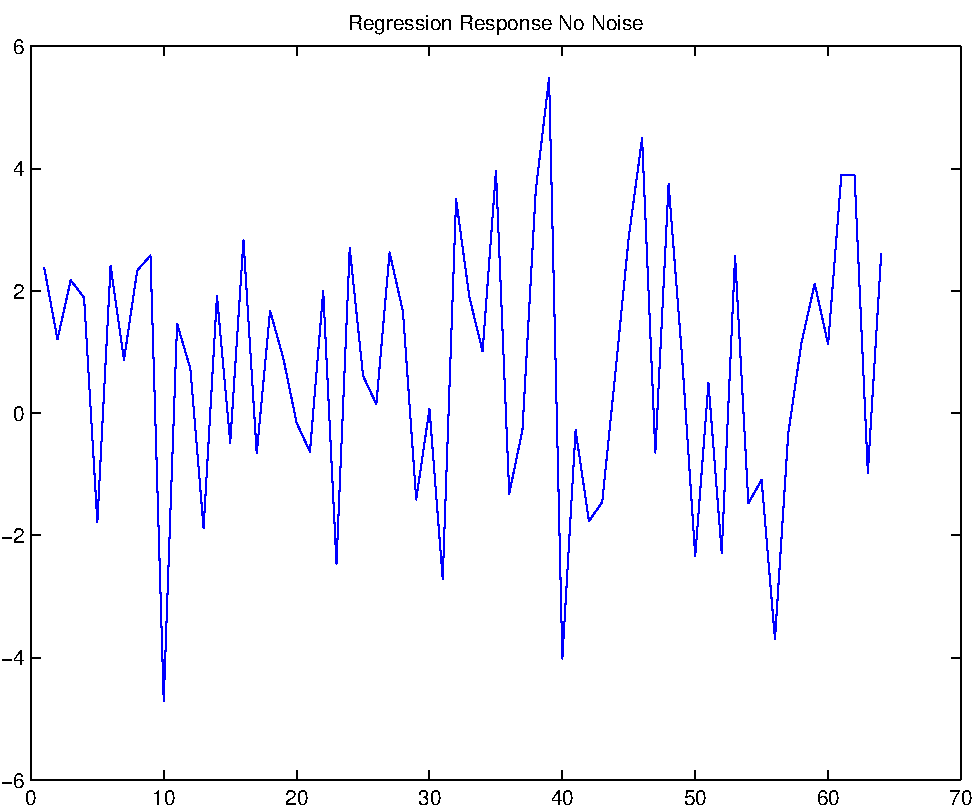
\includegraphics[width=10.0cm,height=10.0cm]{regression_response_no_noise.pdf}

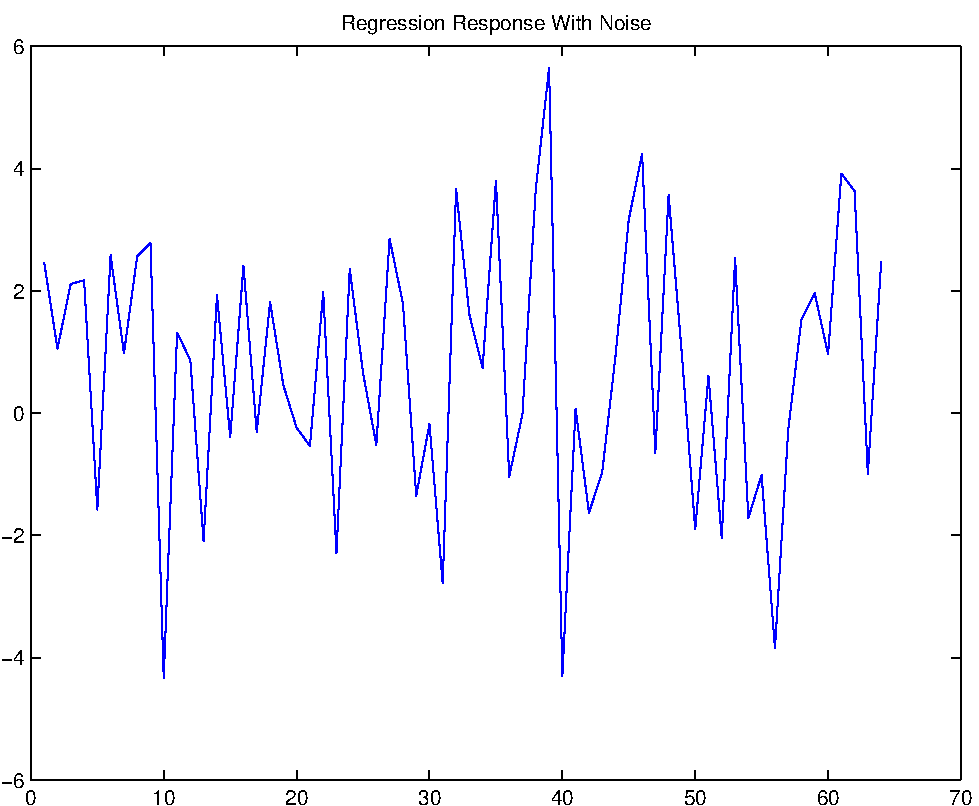
\includegraphics[width=10.0cm,height=10.0cm]{regression_response_with_noise.pdf}

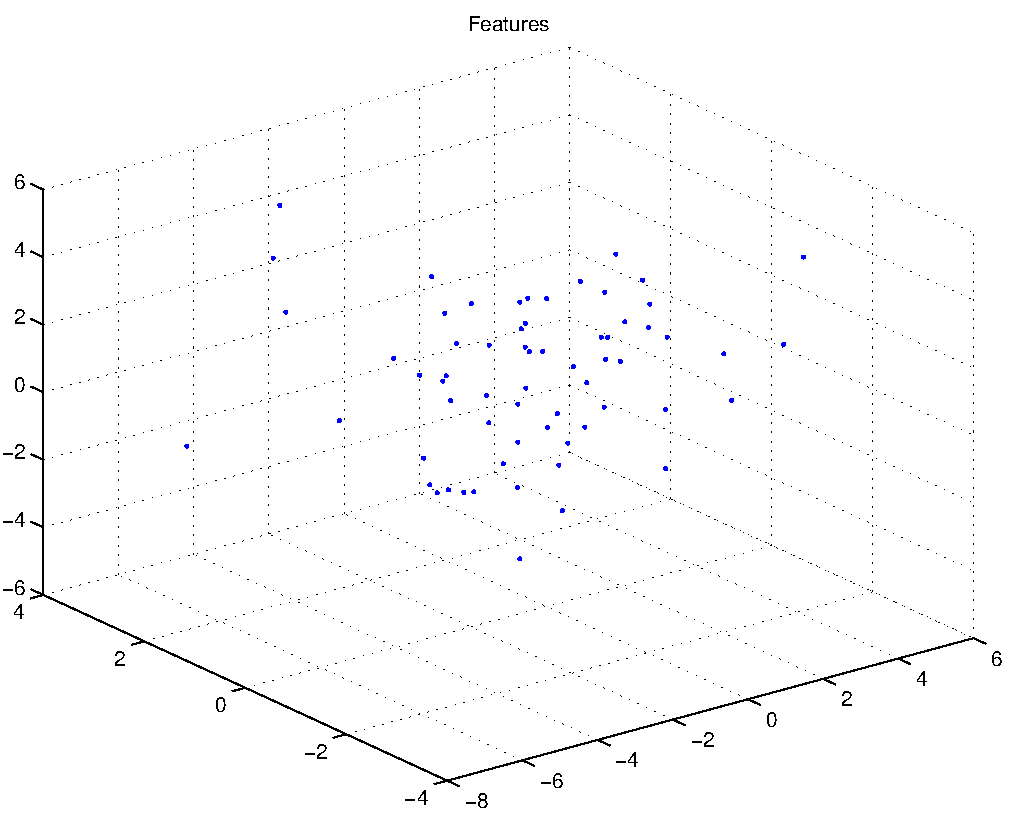
\includegraphics[width=10.0cm,height=10.0cm]{regression_features.pdf}

Beta
+0.817, +0.999, +0.510

Response
+2.463
+1.053
+2.113
+2.172
-1.579
+2.584
+0.976
+2.566
+2.785
-4.338
+1.319
+0.865
-2.100
+1.931
-0.394
+2.410
-0.311
+1.817
+0.458
-0.239
-0.538
+1.979
-2.294
+2.359
+0.652
-0.523
+2.852
+1.788
-1.352
-0.181
-2.786
+3.664
+1.615
+0.739
+3.805
-1.041
-0.017
+3.651
+5.649
-4.307
+0.074
-1.631
-0.965
+0.930
+3.163
+4.241
-0.650
+3.570
+0.939
-1.903
+0.610
-2.049
+2.536
-1.714
-1.016
-3.850
-0.274
+1.533
+1.959
+0.962
+3.920
+3.633
-0.995
+2.486
Estimate for Beta
+0.812
+1.004
+0.484
Error:
-0.005, +0.005, -0.026


QueryPerformanceCounter  =  +4.194
\subsubsection{Fast Gauss Transform}
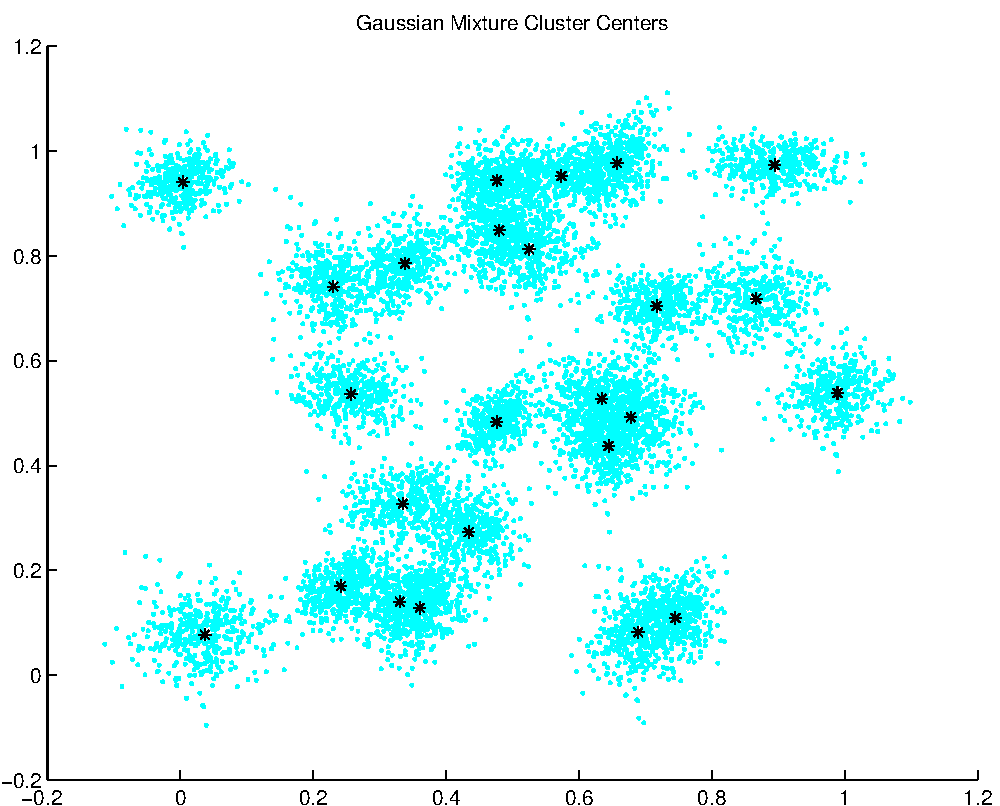
\includegraphics[width=10.0cm,height=10.0cm]{GaussianMixture_ClusterCenters25_Centers.pdf}

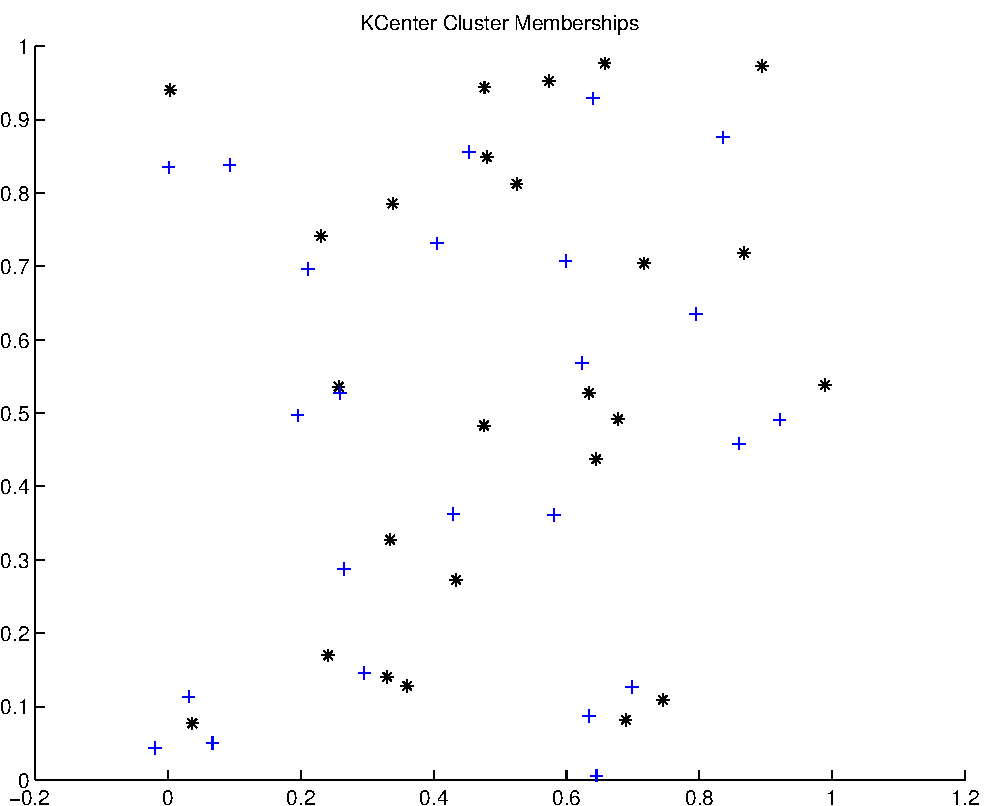
\includegraphics[width=10.0cm,height=10.0cm]{KCenterClusterMemberships_25_Centers.pdf}

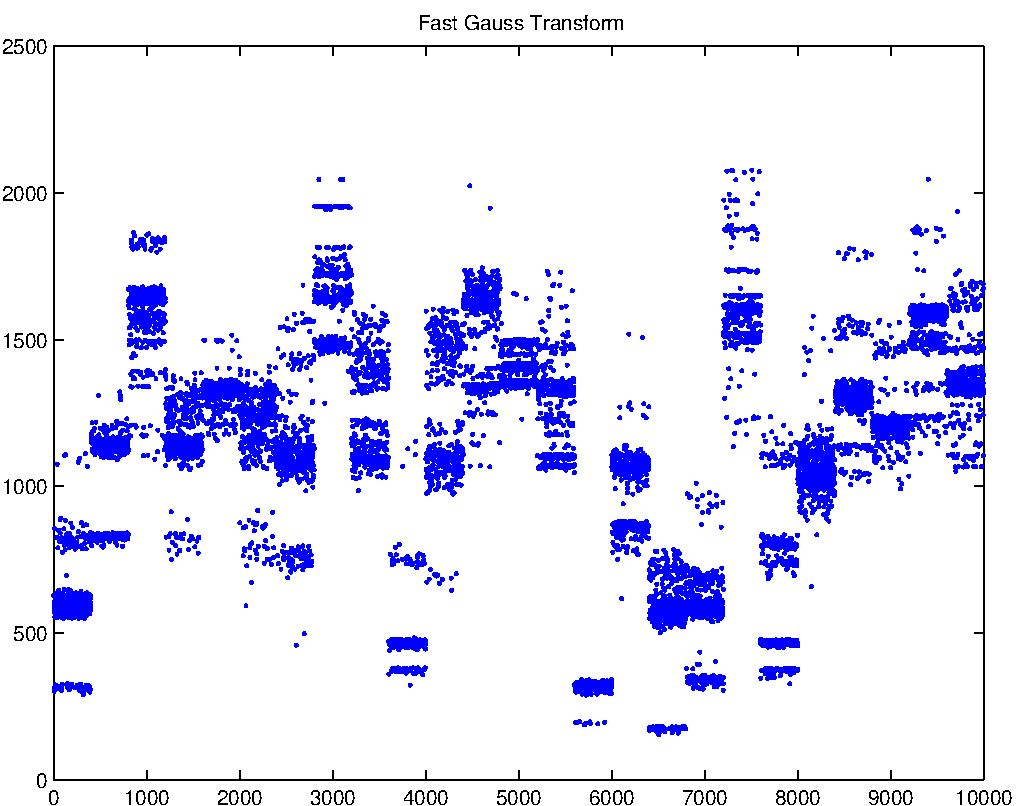
\includegraphics[width=10.0cm,height=10.0cm]{FGT25_Centers.pdf}

QueryPerformanceCounter  =  +6.518
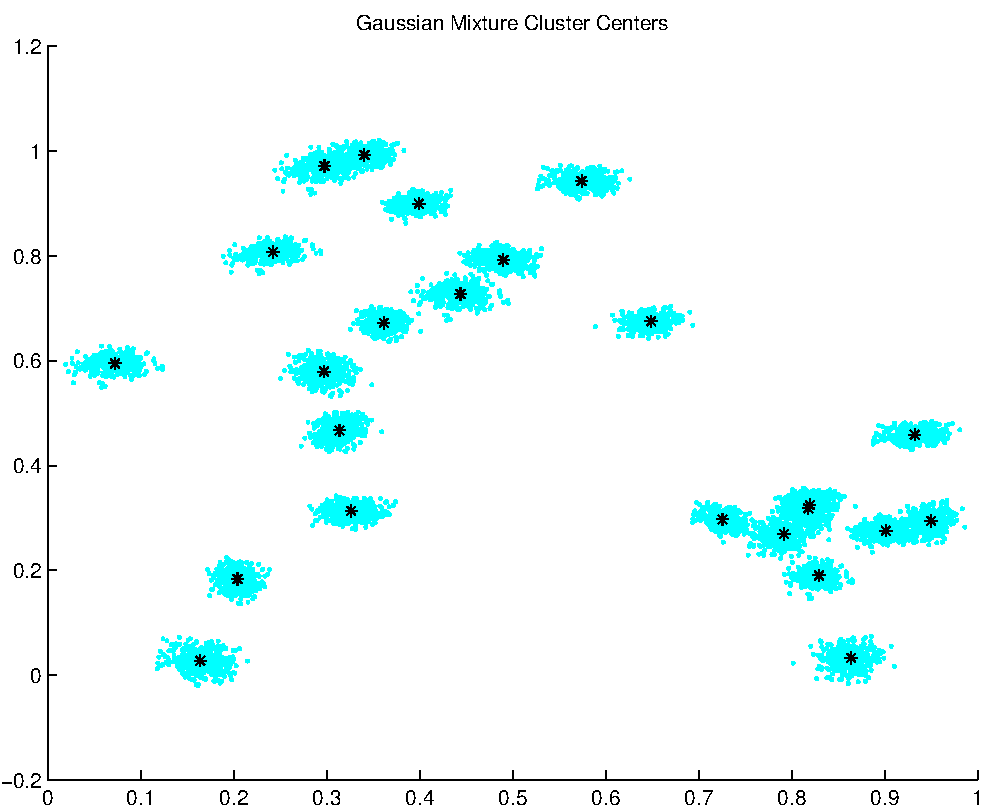
\includegraphics[width=10.0cm,height=10.0cm]{GaussianMixture_ClusterCenters24_Centers.pdf}

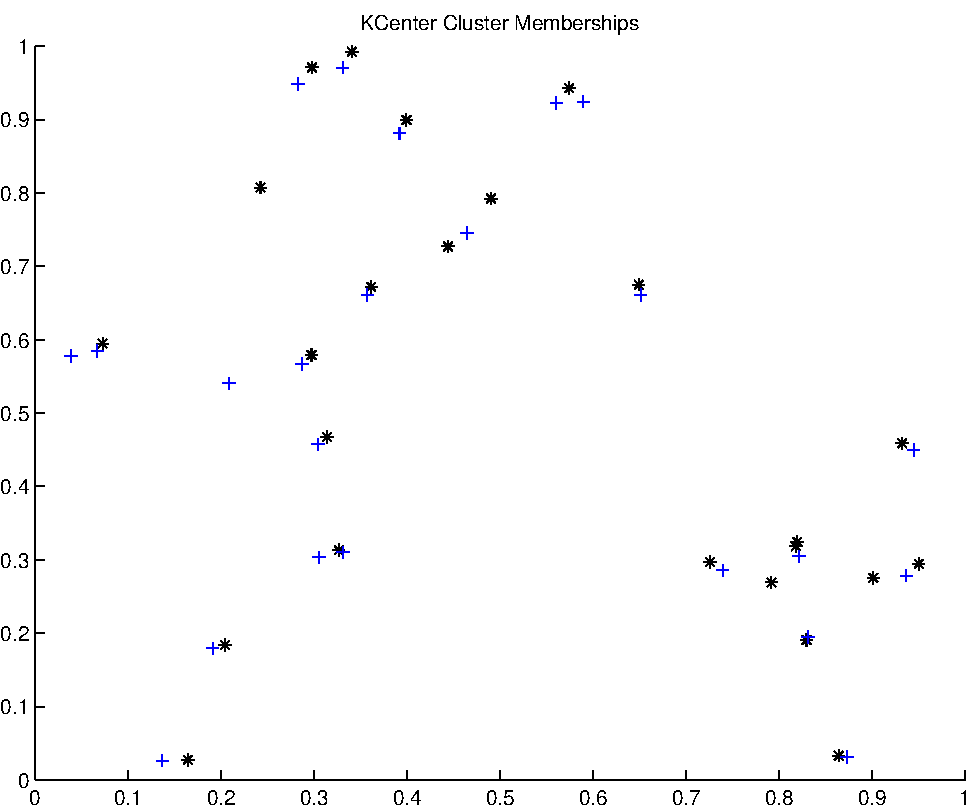
\includegraphics[width=10.0cm,height=10.0cm]{KCenterClusterMemberships_24_Centers.pdf}

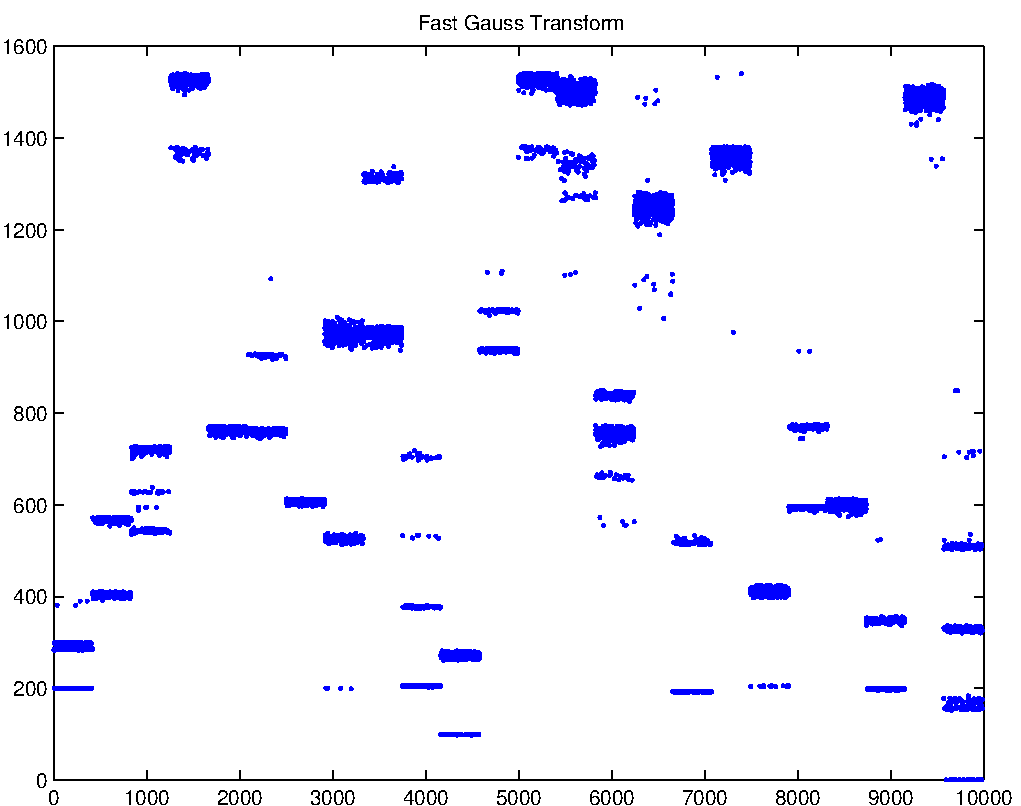
\includegraphics[width=10.0cm,height=10.0cm]{FGT24_Centers.pdf}

QueryPerformanceCounter  =  +6.948
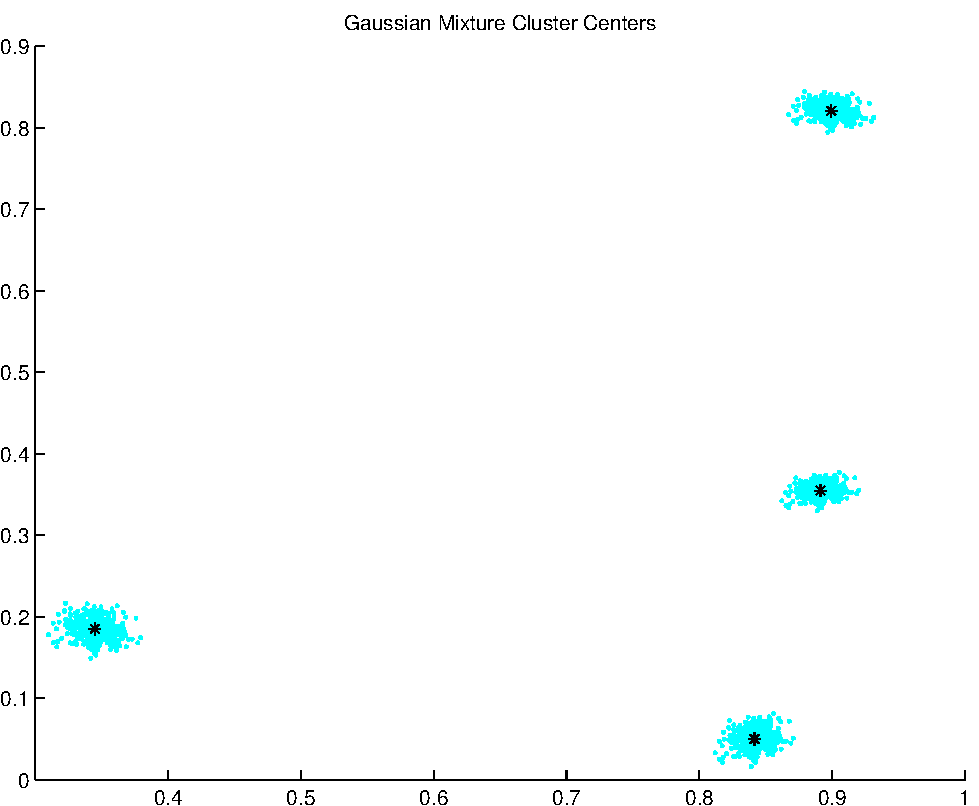
\includegraphics[width=10.0cm,height=10.0cm]{GaussianMixture_ClusterCenters4_Centers.pdf}

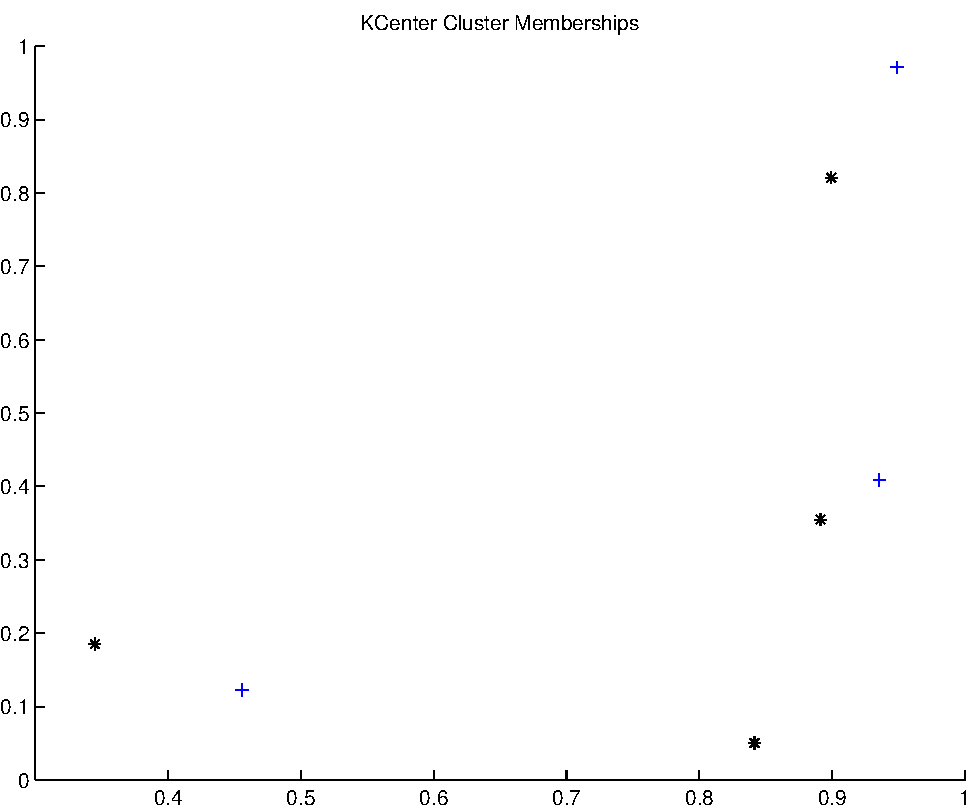
\includegraphics[width=10.0cm,height=10.0cm]{KCenterClusterMemberships_4_Centers.pdf}

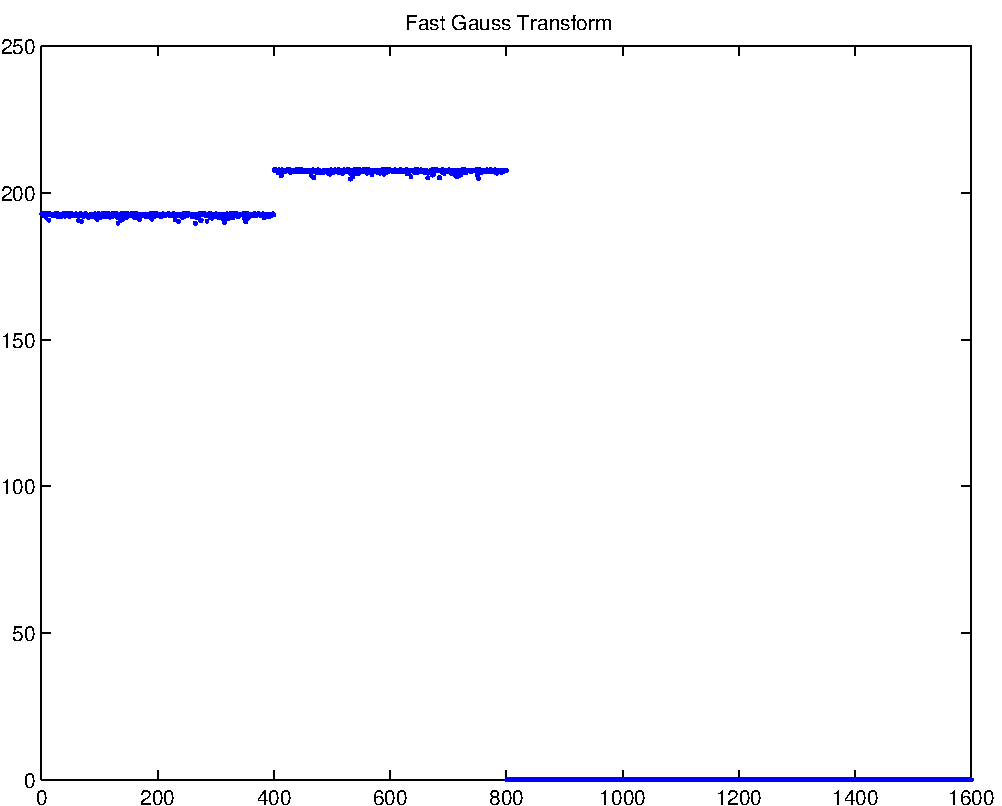
\includegraphics[width=10.0cm,height=10.0cm]{FGT4_Centers.pdf}

QueryPerformanceCounter  =  +3.846
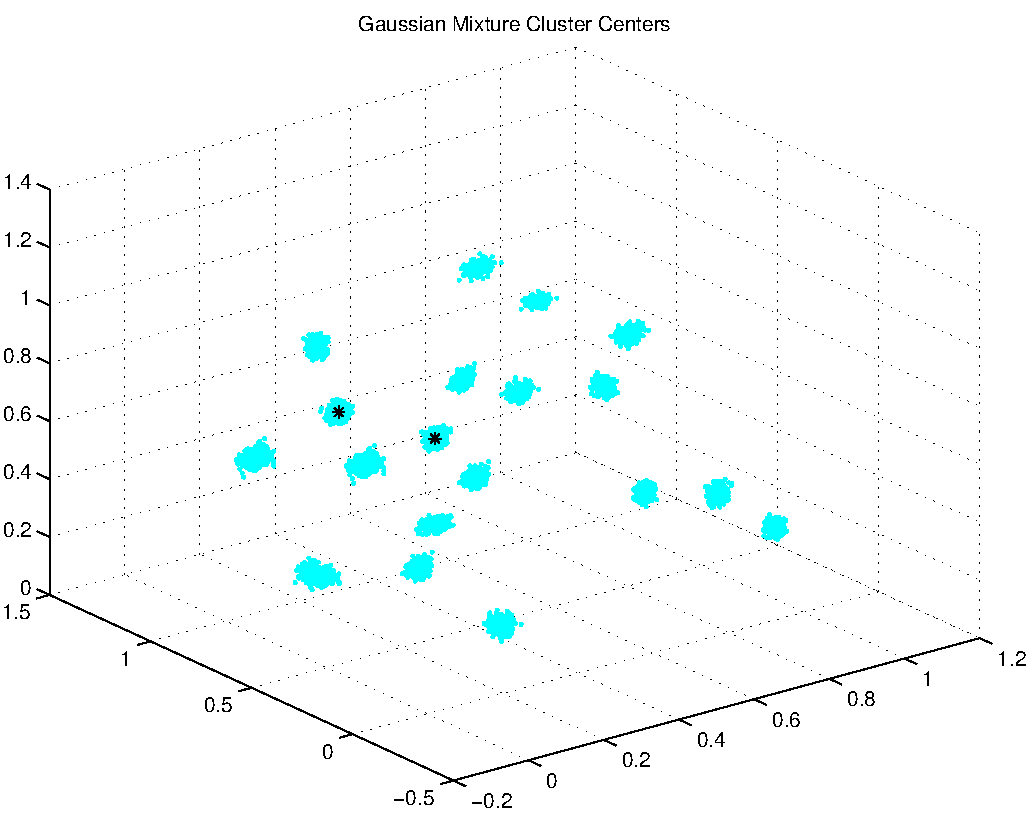
\includegraphics[width=10.0cm,height=10.0cm]{GaussianMixture_ClusterCenters20_Centers.pdf}

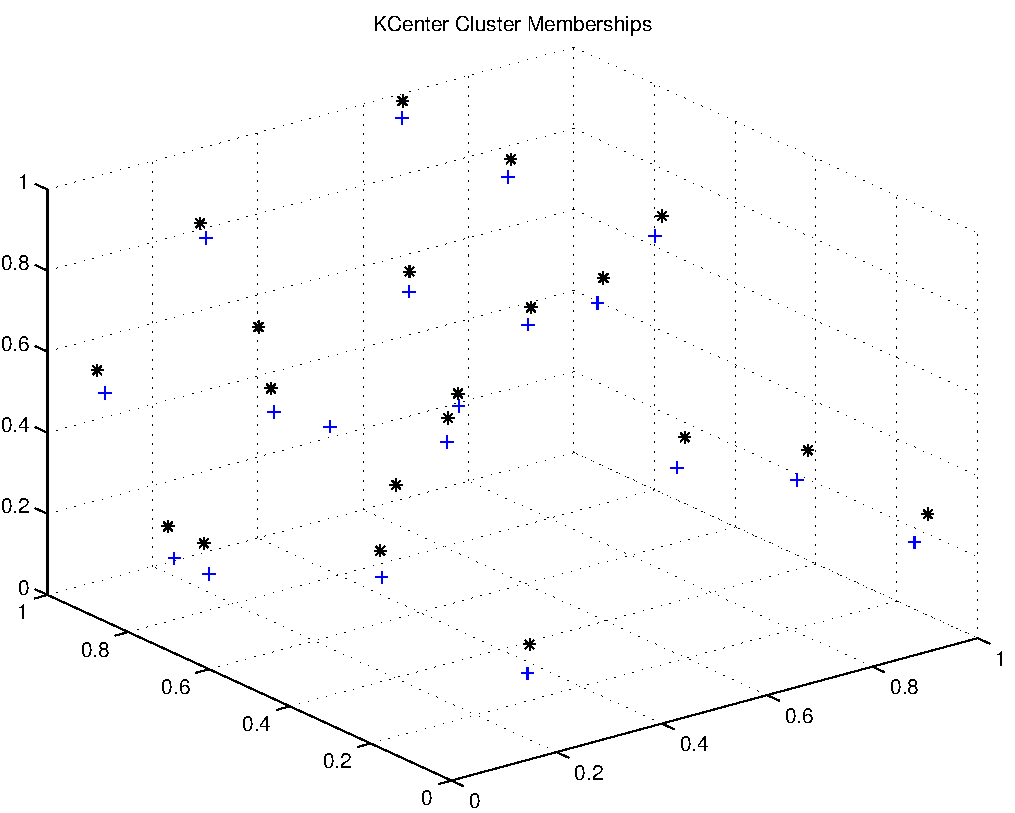
\includegraphics[width=10.0cm,height=10.0cm]{KCenterClusterMemberships_20_Centers.pdf}

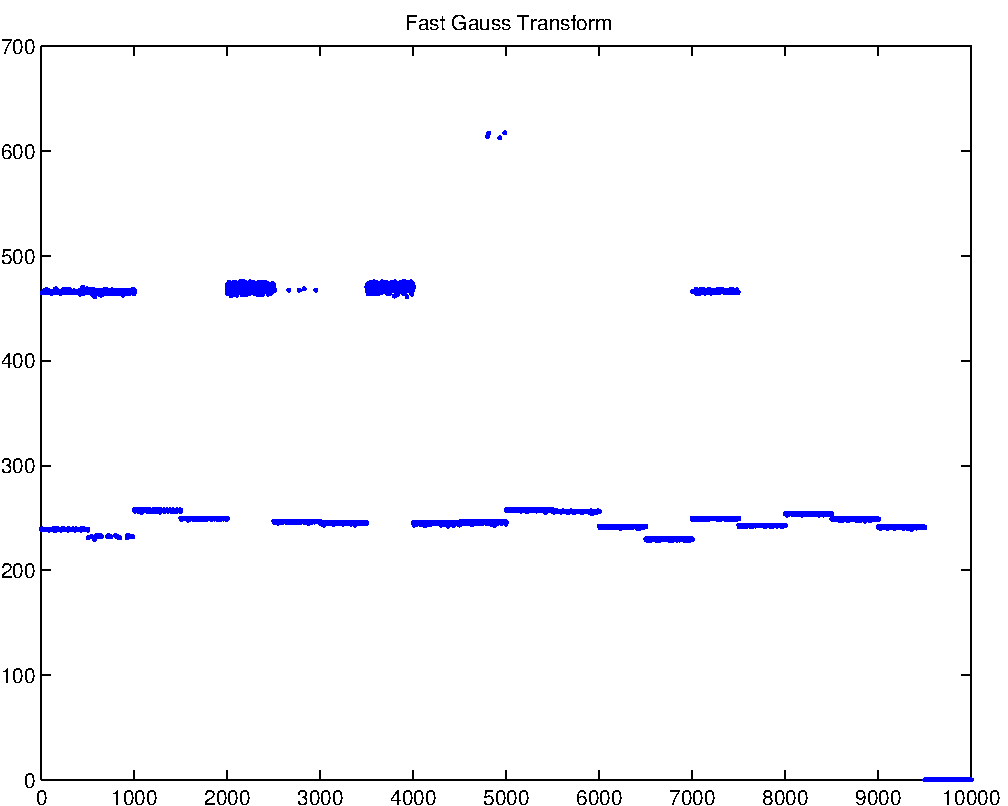
\includegraphics[width=10.0cm,height=10.0cm]{FGT20_Centers.pdf}

QueryPerformanceCounter  =  +6.445
\subsubsection{Matrix Norms}
\subsubsection{Haar Distributed Random Orthogonal Matrix $A \in O(n)$}
 Testing Operator Norm
Number of Dimensions: +12

$A = \left(
\begin{array}{
cccccccccccc}
+0.167 & -0.040 & -0.084 & -0.017 & +0.402 & -0.371 & +0.167 & -0.088 & +0.587 & +0.093 & -0.434 & +0.296 \\
-0.425 & -0.489 & -0.431 & +0.091 & -0.091 & -0.284 & -0.411 & -0.245 & +0.126 & -0.159 & +0.164 & +0.022 \\
+0.369 & -0.223 & -0.035 & +0.506 & -0.205 & -0.469 & +0.125 & +0.049 & -0.473 & +0.148 & -0.130 & +0.117 \\
-0.207 & -0.179 & +0.343 & +0.376 & -0.493 & +0.209 & +0.143 & -0.159 & +0.392 & +0.134 & -0.310 & -0.257 \\
-0.055 & +0.053 & +0.041 & +0.589 & +0.550 & +0.229 & +0.158 & -0.379 & -0.010 & +0.003 & +0.345 & -0.054 \\
-0.045 & +0.590 & -0.106 & +0.020 & -0.002 & -0.291 & -0.306 & -0.398 & -0.122 & +0.069 & -0.293 & -0.442 \\
+0.144 & -0.054 & +0.212 & +0.196 & +0.126 & +0.227 & -0.409 & +0.049 & -0.108 & -0.669 & -0.413 & +0.160 \\
-0.523 & +0.361 & -0.023 & +0.287 & -0.005 & -0.300 & +0.254 & +0.510 & +0.054 & -0.307 & +0.033 & +0.032 \\
+0.343 & -0.004 & -0.387 & -0.072 & -0.211 & +0.009 & +0.471 & -0.190 & +0.137 & -0.557 & +0.091 & -0.296 \\
-0.159 & +0.169 & +0.384 & -0.183 & -0.244 & -0.209 & +0.176 & -0.529 & -0.101 & -0.201 & +0.162 & +0.524 \\
-0.391 & -0.330 & +0.030 & -0.259 & +0.293 & +0.028 & +0.396 & -0.128 & -0.436 & -0.027 & -0.423 & -0.202 \\
+0.131 & -0.237 & +0.576 & -0.139 & +0.191 & -0.441 & -0.089 & +0.089 & +0.121 & -0.168 & +0.286 & -0.452 \\
\end{array}
\right)$ \newline 

$Det(A) :   A \in O(n)$ = (-1.000,+0.000)

$L = \left(
\begin{array}{
cccccccccccc}
+1.000 & +0.000 & +0.000 & +0.000 & +0.000 & +0.000 & +0.000 & +0.000 & +0.000 & +0.000 & +0.000 & +0.000 \\
+0.814 & +1.000 & +0.000 & +0.000 & +0.000 & +0.000 & +0.000 & +0.000 & +0.000 & +0.000 & +0.000 & +0.000 \\
-0.250 & +0.188 & +1.000 & +0.000 & +0.000 & +0.000 & +0.000 & +0.000 & +0.000 & +0.000 & +0.000 & +0.000 \\
-0.707 & -0.041 & -0.105 & +1.000 & +0.000 & +0.000 & +0.000 & +0.000 & +0.000 & +0.000 & +0.000 & +0.000 \\
+0.104 & -0.019 & +0.055 & +0.799 & +1.000 & +0.000 & +0.000 & +0.000 & +0.000 & +0.000 & +0.000 & +0.000 \\
+0.397 & +0.412 & +0.806 & +0.505 & -0.762 & +1.000 & +0.000 & +0.000 & +0.000 & +0.000 & +0.000 & +0.000 \\
+0.748 & +0.767 & +0.561 & -0.489 & +0.224 & +0.007 & +1.000 & +0.000 & +0.000 & +0.000 & +0.000 & +0.000 \\
+0.304 & -0.075 & +0.555 & -0.370 & -0.629 & +0.246 & +0.047 & +1.000 & +0.000 & +0.000 & +0.000 & +0.000 \\
-0.320 & -0.097 & -0.203 & +0.076 & +0.650 & -0.606 & +0.319 & +0.215 & +1.000 & +0.000 & +0.000 & +0.000 \\
-0.657 & -0.299 & -0.810 & +0.060 & -0.089 & -0.273 & +0.624 & +0.322 & +0.959 & +1.000 & +0.000 & +0.000 \\
-0.275 & -0.058 & +0.281 & +0.397 & +0.200 & +0.225 & -0.614 & -0.440 & -0.682 & +0.553 & +1.000 & +0.000 \\
+0.086 & -0.715 & -0.615 & -0.187 & +0.039 & -0.435 & -0.829 & +0.956 & -0.220 & -0.470 & +0.362 & +1.000 \\
\end{array}
\right)$ \newline 

$U = \left(
\begin{array}{
cccccccccccc}
-0.523 & +0.361 & -0.023 & +0.287 & -0.005 & -0.300 & +0.254 & +0.510 & +0.054 & -0.307 & +0.033 & +0.032 \\
+0.000 & -0.782 & -0.412 & -0.142 & -0.088 & -0.040 & -0.617 & -0.660 & +0.082 & +0.090 & +0.137 & -0.004 \\
+0.000 & +0.000 & +0.648 & -0.041 & +0.206 & -0.508 & +0.091 & +0.340 & +0.119 & -0.261 & +0.269 & -0.443 \\
+0.000 & +0.000 & +0.000 & +0.699 & -0.191 & -0.737 & +0.288 & +0.417 & -0.419 & -0.093 & -0.073 & +0.093 \\
+0.000 & +0.000 & +0.000 & +0.000 & +0.690 & +0.877 & -0.116 & -0.797 & +0.314 & +0.125 & +0.387 & -0.106 \\
+0.000 & +0.000 & +0.000 & +0.000 & +0.000 & +1.794 & -0.011 & -1.181 & +0.692 & +0.571 & -0.264 & -0.038 \\
+0.000 & +0.000 & +0.000 & +0.000 & +0.000 & +0.000 & +0.796 & +0.197 & -0.885 & +0.203 & -0.824 & +0.095 \\
+0.000 & +0.000 & +0.000 & +0.000 & +0.000 & +0.000 & +0.000 & -0.989 & -0.262 & -0.062 & +0.334 & +0.733 \\
+0.000 & +0.000 & +0.000 & +0.000 & +0.000 & +0.000 & +0.000 & +0.000 & +1.221 & +0.172 & -0.571 & +0.067 \\
+0.000 & +0.000 & +0.000 & +0.000 & +0.000 & +0.000 & +0.000 & +0.000 & +0.000 & -1.042 & +1.292 & -1.021 \\
+0.000 & +0.000 & +0.000 & +0.000 & +0.000 & +0.000 & +0.000 & +0.000 & +0.000 & +0.000 & -1.925 & +1.277 \\
+0.000 & +0.000 & +0.000 & +0.000 & +0.000 & +0.000 & +0.000 & +0.000 & +0.000 & +0.000 & +0.000 & -2.264 \\
\end{array}
\right)$ \newline 

$L * U  = \left(
\begin{array}{
cccccccccccc}
-0.523 & +0.361 & -0.023 & +0.287 & -0.005 & -0.300 & +0.254 & +0.510 & +0.054 & -0.307 & +0.033 & +0.032 \\
-0.425 & -0.489 & -0.431 & +0.091 & -0.091 & -0.284 & -0.411 & -0.245 & +0.126 & -0.159 & +0.164 & +0.022 \\
+0.131 & -0.237 & +0.576 & -0.139 & +0.191 & -0.441 & -0.089 & +0.089 & +0.121 & -0.168 & +0.286 & -0.452 \\
+0.369 & -0.223 & -0.035 & +0.506 & -0.205 & -0.469 & +0.125 & +0.049 & -0.473 & +0.148 & -0.130 & +0.117 \\
-0.055 & +0.053 & +0.041 & +0.589 & +0.550 & +0.229 & +0.158 & -0.379 & -0.010 & +0.003 & +0.345 & -0.054 \\
-0.207 & -0.179 & +0.343 & +0.376 & -0.493 & +0.209 & +0.143 & -0.159 & +0.392 & +0.134 & -0.310 & -0.257 \\
-0.391 & -0.330 & +0.030 & -0.259 & +0.293 & +0.028 & +0.396 & -0.128 & -0.436 & -0.027 & -0.423 & -0.202 \\
-0.159 & +0.169 & +0.384 & -0.183 & -0.244 & -0.209 & +0.176 & -0.529 & -0.101 & -0.201 & +0.162 & +0.524 \\
+0.167 & -0.040 & -0.084 & -0.017 & +0.402 & -0.371 & +0.167 & -0.088 & +0.587 & +0.093 & -0.434 & +0.296 \\
+0.343 & -0.004 & -0.387 & -0.072 & -0.211 & +0.009 & +0.471 & -0.190 & +0.137 & -0.557 & +0.091 & -0.296 \\
+0.144 & -0.054 & +0.212 & +0.196 & +0.126 & +0.227 & -0.409 & +0.049 & -0.108 & -0.669 & -0.413 & +0.160 \\
-0.045 & +0.590 & -0.106 & +0.020 & -0.002 & -0.291 & -0.306 & -0.398 & -0.122 & +0.069 & -0.293 & -0.442 \\
\end{array}
\right)$ \newline 

$Det(L) :    = (+1.000,+0.000)     Det(U) :    = (+1.000,+0.000)     Det(LU) :    = (+1.000,+0.000)$

$||A||_{L_1}$  = +3.103

$||A||_{L_{\infty}}$ = +3.202

$||A^{-1}||_{L_1}$  = +3.202

$||A^{-1}||_{L_{\infty}}$ = +3.103

$||A||_{L_{\infty}} * ||A^{-1}||_{L_{\infty}} = +9.933$

$||A||_{L_1} * ||A^{-1}||_{L_1} = +9.933$

Frobenious Norm  $||A||_{\textit{F}}$ via $\sum\limits_{i,j =0}^{n} \|A_{i,j}|$   of  $A \in O(n)$  +3.464

$L_1$ condition number of Haar Distributed Random Orthogonal Matrix $A \in O(n)$ +9.933

$A = \left(
\begin{array}{
cccccccccccc}
+0.167 & -0.040 & -0.084 & -0.017 & +0.402 & -0.371 & +0.167 & -0.088 & +0.587 & +0.093 & -0.434 & +0.296 \\
-0.425 & -0.489 & -0.431 & +0.091 & -0.091 & -0.284 & -0.411 & -0.245 & +0.126 & -0.159 & +0.164 & +0.022 \\
+0.369 & -0.223 & -0.035 & +0.506 & -0.205 & -0.469 & +0.125 & +0.049 & -0.473 & +0.148 & -0.130 & +0.117 \\
-0.207 & -0.179 & +0.343 & +0.376 & -0.493 & +0.209 & +0.143 & -0.159 & +0.392 & +0.134 & -0.310 & -0.257 \\
-0.055 & +0.053 & +0.041 & +0.589 & +0.550 & +0.229 & +0.158 & -0.379 & -0.010 & +0.003 & +0.345 & -0.054 \\
-0.045 & +0.590 & -0.106 & +0.020 & -0.002 & -0.291 & -0.306 & -0.398 & -0.122 & +0.069 & -0.293 & -0.442 \\
+0.144 & -0.054 & +0.212 & +0.196 & +0.126 & +0.227 & -0.409 & +0.049 & -0.108 & -0.669 & -0.413 & +0.160 \\
-0.523 & +0.361 & -0.023 & +0.287 & -0.005 & -0.300 & +0.254 & +0.510 & +0.054 & -0.307 & +0.033 & +0.032 \\
+0.343 & -0.004 & -0.387 & -0.072 & -0.211 & +0.009 & +0.471 & -0.190 & +0.137 & -0.557 & +0.091 & -0.296 \\
-0.159 & +0.169 & +0.384 & -0.183 & -0.244 & -0.209 & +0.176 & -0.529 & -0.101 & -0.201 & +0.162 & +0.524 \\
-0.391 & -0.330 & +0.030 & -0.259 & +0.293 & +0.028 & +0.396 & -0.128 & -0.436 & -0.027 & -0.423 & -0.202 \\
+0.131 & -0.237 & +0.576 & -0.139 & +0.191 & -0.441 & -0.089 & +0.089 & +0.121 & -0.168 & +0.286 & -0.452 \\
\end{array}
\right)$ \newline 

$L_{\infty}$ condition number of Haar Distributed Random Orthogonal Matrix $A \in O(n)$ +9.006

Eigenvalues of $A \in O(n)$

(+0.642,+0.767), (+0.642,-0.767), (-0.287,+0.958), (-0.287,-0.958), (-1.000,+0.000), (-0.707,+0.707), (-0.707,-0.707), (-0.876,+0.482), (-0.876,-0.482), (+1.000,+0.000), (+0.948,+0.318), (+0.948,-0.318)

 $|\lambda | : \lambda \in \sigma(A) , A \in O(n)$

+1.000, +1.000, +1.000, +1.000, +1.000, +1.000, +1.000, +1.000, +1.000, +1.000, +1.000, +1.000


Calculating $A^{\dag} A,$  we expect $A^{\dag} A \approx I$

$A^{\dag} A = \left(
\begin{array}{
cccccccccccc}
+1.000 & +0.000 & -0.000 & +0.000 & -0.000 & +0.000 & -0.000 & +0.000 & +0.000 & -0.000 & +0.000 & +0.000 \\
+0.000 & +1.000 & +0.000 & -0.000 & -0.000 & -0.000 & -0.000 & +0.000 & -0.000 & -0.000 & +0.000 & +0.000 \\
-0.000 & +0.000 & +1.000 & -0.000 & +0.000 & +0.000 & -0.000 & -0.000 & +0.000 & -0.000 & -0.000 & +0.000 \\
+0.000 & -0.000 & -0.000 & +1.000 & +0.000 & -0.000 & -0.000 & -0.000 & -0.000 & -0.000 & +0.000 & +0.000 \\
-0.000 & -0.000 & +0.000 & +0.000 & +1.000 & +0.000 & +0.000 & -0.000 & +0.000 & +0.000 & -0.000 & -0.000 \\
+0.000 & -0.000 & +0.000 & -0.000 & +0.000 & +1.000 & +0.000 & +0.000 & -0.000 & -0.000 & +0.000 & +0.000 \\
-0.000 & -0.000 & -0.000 & -0.000 & +0.000 & +0.000 & +1.000 & -0.000 & -0.000 & +0.000 & +0.000 & +0.000 \\
+0.000 & +0.000 & -0.000 & -0.000 & -0.000 & +0.000 & -0.000 & +1.000 & +0.000 & +0.000 & -0.000 & -0.000 \\
+0.000 & -0.000 & +0.000 & -0.000 & +0.000 & -0.000 & -0.000 & +0.000 & +1.000 & -0.000 & +0.000 & +0.000 \\
-0.000 & -0.000 & -0.000 & -0.000 & +0.000 & -0.000 & +0.000 & +0.000 & -0.000 & +1.000 & +0.000 & -0.000 \\
+0.000 & +0.000 & -0.000 & +0.000 & -0.000 & +0.000 & +0.000 & -0.000 & +0.000 & +0.000 & +1.000 & +0.000 \\
+0.000 & +0.000 & +0.000 & +0.000 & -0.000 & +0.000 & +0.000 & -0.000 & +0.000 & -0.000 & +0.000 & +1.000 \\
\end{array}
\right)$ \newline 

Calculating $A^{-1} ,  A \in O(n)$.

$A^{-1} = \left(
\begin{array}{
cccccccccccc}
+0.167 & -0.425 & +0.369 & -0.207 & -0.055 & -0.045 & +0.144 & -0.523 & +0.343 & -0.159 & -0.391 & +0.131 \\
-0.040 & -0.489 & -0.223 & -0.179 & +0.053 & +0.590 & -0.054 & +0.361 & -0.004 & +0.169 & -0.330 & -0.237 \\
-0.084 & -0.431 & -0.035 & +0.343 & +0.041 & -0.106 & +0.212 & -0.023 & -0.387 & +0.384 & +0.030 & +0.576 \\
-0.017 & +0.091 & +0.506 & +0.376 & +0.589 & +0.020 & +0.196 & +0.287 & -0.072 & -0.183 & -0.259 & -0.139 \\
+0.402 & -0.091 & -0.205 & -0.493 & +0.550 & -0.002 & +0.126 & -0.005 & -0.211 & -0.244 & +0.293 & +0.191 \\
-0.371 & -0.284 & -0.469 & +0.209 & +0.229 & -0.291 & +0.227 & -0.300 & +0.009 & -0.209 & +0.028 & -0.441 \\
+0.167 & -0.411 & +0.125 & +0.143 & +0.158 & -0.306 & -0.409 & +0.254 & +0.471 & +0.176 & +0.396 & -0.089 \\
-0.088 & -0.245 & +0.049 & -0.159 & -0.379 & -0.398 & +0.049 & +0.510 & -0.190 & -0.529 & -0.128 & +0.089 \\
+0.587 & +0.126 & -0.473 & +0.392 & -0.010 & -0.122 & -0.108 & +0.054 & +0.137 & -0.101 & -0.436 & +0.121 \\
+0.093 & -0.159 & +0.148 & +0.134 & +0.003 & +0.069 & -0.669 & -0.307 & -0.557 & -0.201 & -0.027 & -0.168 \\
-0.434 & +0.164 & -0.130 & -0.310 & +0.345 & -0.293 & -0.413 & +0.033 & +0.091 & +0.162 & -0.423 & +0.286 \\
+0.296 & +0.022 & +0.117 & -0.257 & -0.054 & -0.442 & +0.160 & +0.032 & -0.296 & +0.524 & -0.202 & -0.452 \\
\end{array}
\right)$ \newline 

Calculating $A^{-1} *A  ,  A \in O(n)$.   We expect $A^{-1} *A  \approx I$. 

$A^{-1} *A = \left(
\begin{array}{
cccccccccccc}
+1.000 & +0.000 & +0.000 & +0.000 & -0.000 & -0.000 & +0.000 & +0.000 & -0.000 & -0.000 & -0.000 & +0.000 \\
+0.000 & +1.000 & -0.000 & -0.000 & -0.000 & +0.000 & -0.000 & -0.000 & -0.000 & +0.000 & +0.000 & -0.000 \\
+0.000 & +0.000 & +1.000 & +0.000 & -0.000 & +0.000 & +0.000 & +0.000 & +0.000 & +0.000 & +0.000 & -0.000 \\
-0.000 & +0.000 & +0.000 & +1.000 & +0.000 & +0.000 & +0.000 & -0.000 & +0.000 & +0.000 & +0.000 & -0.000 \\
+0.000 & +0.000 & +0.000 & -0.000 & +1.000 & +0.000 & -0.000 & -0.000 & +0.000 & +0.000 & +0.000 & +0.000 \\
+0.000 & +0.000 & +0.000 & +0.000 & +0.000 & +1.000 & -0.000 & -0.000 & +0.000 & -0.000 & -0.000 & +0.000 \\
-0.000 & +0.000 & +0.000 & +0.000 & +0.000 & +0.000 & +1.000 & -0.000 & -0.000 & -0.000 & -0.000 & -0.000 \\
+0.000 & -0.000 & -0.000 & -0.000 & -0.000 & -0.000 & -0.000 & +1.000 & +0.000 & +0.000 & -0.000 & -0.000 \\
-0.000 & -0.000 & +0.000 & +0.000 & +0.000 & +0.000 & -0.000 & -0.000 & +1.000 & +0.000 & +0.000 & +0.000 \\
+0.000 & +0.000 & +0.000 & +0.000 & +0.000 & -0.000 & -0.000 & -0.000 & +0.000 & +1.000 & -0.000 & -0.000 \\
-0.000 & -0.000 & +0.000 & +0.000 & +0.000 & -0.000 & -0.000 & +0.000 & -0.000 & -0.000 & +1.000 & +0.000 \\
+0.000 & +0.000 & +0.000 & +0.000 & -0.000 & -0.000 & +0.000 & +0.000 & +0.000 & +0.000 & +0.000 & +1.000 \\
\end{array}
\right)$ \newline 

Calculating SVD of  $A \in O(n)$

$U = \left(
\begin{array}{
cccccccccccc}
-0.254 & +0.661 & +0.123 & +0.090 & +0.076 & -0.316 & -0.419 & -0.219 & -0.070 & +0.373 & +0.040 & +0.023 \\
-0.026 & -0.386 & -0.098 & -0.101 & +0.043 & +0.290 & -0.139 & -0.515 & -0.025 & +0.543 & -0.246 & -0.323 \\
+0.622 & +0.233 & -0.573 & +0.192 & -0.089 & +0.035 & -0.071 & -0.032 & -0.351 & +0.046 & -0.186 & +0.132 \\
-0.417 & -0.037 & -0.188 & +0.239 & -0.685 & -0.195 & +0.146 & -0.031 & +0.050 & -0.039 & -0.444 & +0.048 \\
+0.122 & -0.258 & +0.186 & +0.161 & -0.006 & -0.542 & +0.451 & +0.015 & -0.382 & +0.401 & +0.233 & +0.012 \\
-0.167 & +0.040 & +0.084 & +0.017 & -0.402 & +0.371 & -0.167 & +0.088 & -0.587 & -0.093 & +0.434 & -0.296 \\
-0.059 & +0.020 & +0.176 & -0.095 & +0.242 & -0.018 & -0.090 & +0.588 & -0.320 & +0.092 & -0.586 & -0.299 \\
-0.033 & -0.088 & +0.227 & -0.061 & -0.126 & +0.364 & -0.081 & +0.199 & -0.087 & +0.375 & -0.058 & +0.768 \\
+0.392 & -0.245 & +0.542 & +0.171 & -0.211 & -0.206 & -0.461 & -0.217 & -0.040 & -0.286 & -0.182 & +0.035 \\
-0.328 & -0.122 & -0.122 & -0.257 & +0.315 & -0.128 & +0.009 & -0.378 & -0.511 & -0.389 & -0.157 & +0.319 \\
+0.249 & +0.275 & +0.166 & -0.790 & -0.349 & -0.080 & +0.235 & -0.117 & +0.002 & +0.031 & -0.101 & -0.056 \\
-0.058 & -0.363 & -0.389 & -0.360 & -0.119 & -0.384 & -0.515 & +0.297 & +0.078 & +0.101 & +0.222 & +0.050 \\
\end{array}
\right)$ \newline 

$S = \left(
\begin{array}{
cccccccccccc}
+1.000 & +0.000 & +0.000 & +0.000 & +0.000 & +0.000 & +0.000 & +0.000 & +0.000 & +0.000 & +0.000 & +0.000 \\
+0.000 & +1.000 & +0.000 & +0.000 & +0.000 & +0.000 & +0.000 & +0.000 & +0.000 & +0.000 & +0.000 & +0.000 \\
+0.000 & +0.000 & +1.000 & +0.000 & +0.000 & +0.000 & +0.000 & +0.000 & +0.000 & +0.000 & +0.000 & +0.000 \\
+0.000 & +0.000 & +0.000 & +1.000 & +0.000 & +0.000 & +0.000 & +0.000 & +0.000 & +0.000 & +0.000 & +0.000 \\
+0.000 & +0.000 & +0.000 & +0.000 & +1.000 & +0.000 & +0.000 & +0.000 & +0.000 & +0.000 & +0.000 & +0.000 \\
+0.000 & +0.000 & +0.000 & +0.000 & +0.000 & +1.000 & +0.000 & +0.000 & +0.000 & +0.000 & +0.000 & +0.000 \\
+0.000 & +0.000 & +0.000 & +0.000 & +0.000 & +0.000 & +1.000 & +0.000 & +0.000 & +0.000 & +0.000 & +0.000 \\
+0.000 & +0.000 & +0.000 & +0.000 & +0.000 & +0.000 & +0.000 & +1.000 & +0.000 & +0.000 & +0.000 & +0.000 \\
+0.000 & +0.000 & +0.000 & +0.000 & +0.000 & +0.000 & +0.000 & +0.000 & +1.000 & +0.000 & +0.000 & +0.000 \\
+0.000 & +0.000 & +0.000 & +0.000 & +0.000 & +0.000 & +0.000 & +0.000 & +0.000 & +1.000 & +0.000 & +0.000 \\
+0.000 & +0.000 & +0.000 & +0.000 & +0.000 & +0.000 & +0.000 & +0.000 & +0.000 & +0.000 & +1.000 & +0.000 \\
+0.000 & +0.000 & +0.000 & +0.000 & +0.000 & +0.000 & +0.000 & +0.000 & +0.000 & +0.000 & +0.000 & +1.000 \\
\end{array}
\right)$ \newline 

$V = \left(
\begin{array}{
cccccccccccc}
-0.000 & +0.000 & +0.000 & +0.000 & +0.000 & -1.000 & +0.000 & -0.000 & -0.000 & -0.000 & +0.000 & +0.000 \\
-0.012 & +0.192 & -0.157 & +0.305 & -0.099 & -0.000 & -0.351 & -0.217 & +0.066 & +0.303 & -0.419 & +0.627 \\
-0.044 & -0.073 & +0.499 & +0.264 & +0.701 & -0.000 & +0.102 & +0.016 & +0.343 & -0.000 & -0.232 & +0.000 \\
-0.114 & +0.326 & -0.357 & +0.581 & -0.074 & +0.000 & -0.051 & +0.010 & +0.236 & -0.455 & -0.083 & -0.372 \\
+0.108 & +0.115 & -0.040 & -0.389 & +0.105 & -0.000 & -0.335 & -0.163 & -0.130 & +0.076 & -0.618 & -0.518 \\
+0.710 & +0.200 & +0.241 & +0.148 & -0.159 & +0.000 & +0.142 & -0.521 & +0.095 & +0.076 & +0.173 & -0.116 \\
-0.185 & -0.231 & +0.122 & -0.031 & -0.526 & -0.000 & +0.269 & +0.051 & +0.598 & +0.303 & -0.250 & -0.179 \\
+0.155 & -0.724 & -0.252 & +0.362 & +0.035 & +0.000 & +0.214 & -0.162 & -0.341 & +0.000 & -0.250 & -0.076 \\
-0.538 & -0.169 & +0.283 & +0.104 & -0.092 & +0.000 & -0.346 & -0.594 & -0.092 & +0.000 & +0.273 & -0.160 \\
+0.223 & -0.219 & -0.230 & +0.150 & +0.167 & +0.000 & -0.523 & +0.250 & +0.251 & +0.455 & +0.368 & -0.240 \\
-0.264 & +0.358 & -0.233 & +0.120 & +0.216 & +0.000 & +0.451 & -0.122 & -0.228 & +0.606 & +0.078 & -0.205 \\
-0.030 & -0.126 & -0.523 & -0.384 & +0.309 & +0.000 & +0.130 & -0.441 & +0.445 & -0.152 & +0.102 & +0.156 \\
\end{array}
\right)$ \newline 

$U S V = \left(
\begin{array}{
cccccccccccc}
-0.087 & +0.290 & -0.277 & +0.188 & +0.370 & +0.254 & -0.604 & +0.145 & -0.008 & +0.205 & -0.131 & +0.387 \\
+0.387 & +0.205 & +0.323 & -0.185 & -0.069 & +0.026 & -0.418 & +0.322 & +0.082 & +0.059 & +0.521 & -0.323 \\
+0.268 & +0.152 & -0.516 & -0.041 & -0.377 & -0.622 & -0.111 & +0.124 & -0.008 & -0.154 & +0.026 & +0.236 \\
-0.183 & -0.209 & -0.066 & +0.227 & -0.357 & +0.417 & +0.025 & +0.226 & +0.266 & -0.436 & +0.370 & +0.342 \\
-0.257 & -0.176 & -0.265 & +0.022 & +0.149 & -0.122 & +0.181 & +0.658 & +0.387 & +0.265 & -0.092 & -0.318 \\
+0.448 & +0.322 & +0.002 & +0.383 & +0.084 & +0.167 & +0.564 & +0.245 & -0.207 & +0.217 & +0.103 & +0.188 \\
+0.480 & -0.559 & +0.127 & +0.140 & +0.050 & +0.059 & -0.207 & +0.284 & -0.195 & -0.229 & -0.449 & -0.002 \\
+0.411 & -0.306 & -0.317 & -0.079 & +0.446 & +0.033 & +0.079 & -0.369 & +0.450 & +0.014 & +0.288 & +0.046 \\
-0.154 & +0.167 & +0.284 & +0.073 & +0.564 & -0.392 & +0.089 & +0.176 & +0.005 & -0.569 & +0.101 & +0.133 \\
+0.139 & +0.259 & -0.082 & -0.750 & +0.028 & +0.328 & +0.193 & +0.184 & +0.098 & -0.224 & -0.286 & +0.156 \\
-0.042 & -0.278 & +0.420 & -0.243 & -0.038 & -0.249 & +0.035 & +0.109 & +0.113 & +0.443 & +0.082 & +0.627 \\
-0.162 & -0.307 & -0.313 & -0.279 & +0.193 & +0.058 & +0.044 & +0.143 & -0.684 & +0.033 & +0.415 & +0.007 \\
\end{array}
\right)$ \newline 

\subsubsection{Wishart Matrix $A \in W(n)$}
$L_1$ condition number of Wishart Matrix +56267.800
$L_infty$ condition number of Wishart Matrix +56267.800
\subsubsection{Gaussian Orthogonal Ensemble $A \in GOE(n)$}
$L_1$ condition number of GOE Matrix +470.231
$L_\infty$ condition number of GOE Matrix +470.231
\subsubsection{The Identity Matrix $I \in M(n)$}
$L_1$ condition number of $I$ = +1.000
$L_\infty$ condition number of $I$ = +1.000
QueryPerformanceCounter  =  +0.387
\subsubsection{Principal Components Matlab }
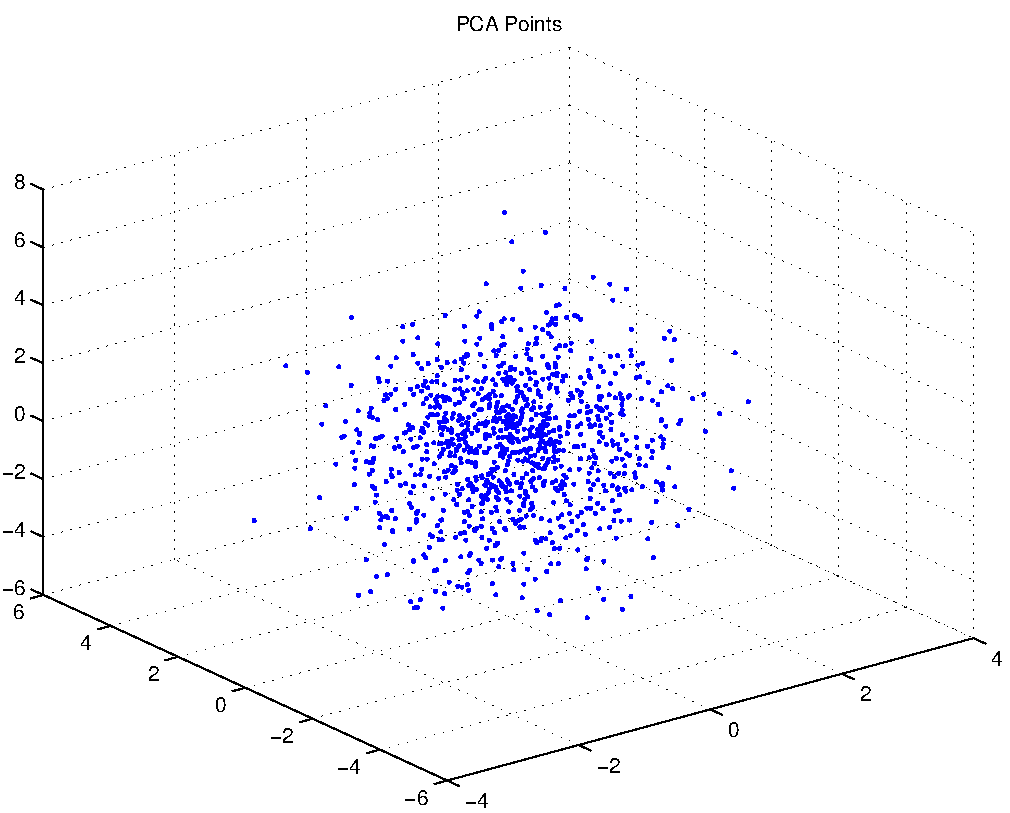
\includegraphics[width=10.0cm,height=10.0cm]{PCAPoints.pdf}

The eigenvectors:
+0.121, +0.241, +0.963
+0.199, +0.944, -0.261
-0.972, +0.224, +0.067

All of the eigenvalues of the covariance matrix:
(+0.958,+0.000), (+2.025,+0.000), (+3.017,+0.000)

QueryPerformanceCounter  =  +1.040
\subsubsection{Multi Variate Random Number Generator }
Sample from $N(\mu,\Sigma)$
mean= -0.002, variance=+1.004, skewness=+0.006, kurtosis=+3.003
mean= -0.001, variance=+1.017, skewness=-0.005, kurtosis=+2.988
mean= -0.002, variance=+1.006, skewness=-0.016, kurtosis=+3.014
Covariance Matrix 
+1.004, +0.009, +0.003
+0.009, +1.017, -0.003
+0.003, -0.003, +1.006

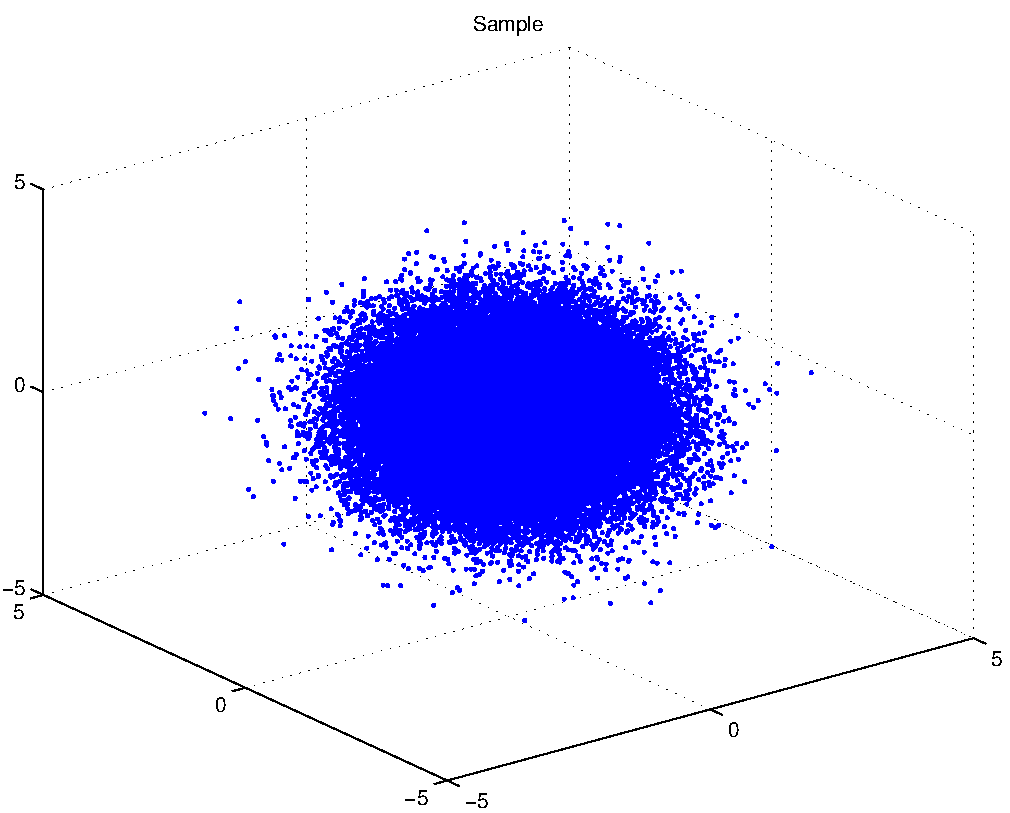
\includegraphics[width=10.0cm,height=10.0cm]{R_3_Normal.pdf}

Generate a sample from a unifom mixture of three Gaussians in $R^3$
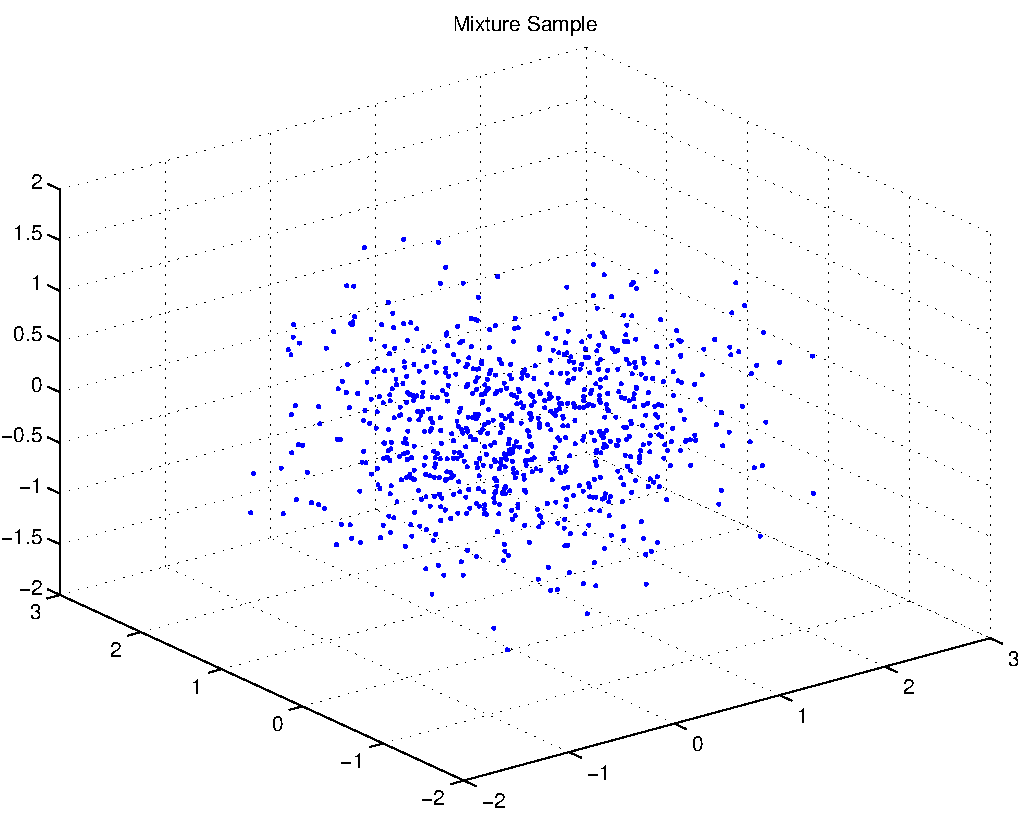
\includegraphics[width=10.0cm,height=10.0cm]{R_3_Normal_Mixture.pdf}

QueryPerformanceCounter  =  +16.975
\subsubsection{Matrix Multiply}
Comparing naive matrix multiply verus Intel MKL dgemm for matrix of size +2048.
This is for type double (hence the d in dgemm).
Naive type double matrix multiply tic toc  =  +0.411
dgemm plus row to column major transpose operation tic toc  =  +0.318
Comparing naive matrix multiply verus Intel MKL sgemm for matrix of size +2048.
This is for type float (hence the s in dgemm).
Naive type float matrix multiply tic toc  =  +0.255
sgemm plus row to column major transpose operation tic toc  =  +0.229
QueryPerformanceCounter  =  +1.336
\subsubsection{Descriptive Statistics}
Mean N(0,1): +0.003
Variance N(0,1): +1.006
Mean N(0,1) [recurrence relation method] :+0.003
Variance [recurrence relation method] :+1.006
Skewness : +0.007
Kurtosis : +2.997
QueryPerformanceCounter  =  +0.032
\subsubsection{Time Series }
+0.093
+0.726
+0.011
+2.178
QueryPerformanceCounter  =  +0.034
QueryPerformanceCounter  =  +6.281
\subsubsection{Iterated Exponential Filtering }
$\mu_1 =+0.093$
$\mu_2 =+0.726$
$\mu_3 =+0.011$
$\mu_4 =+2.178$
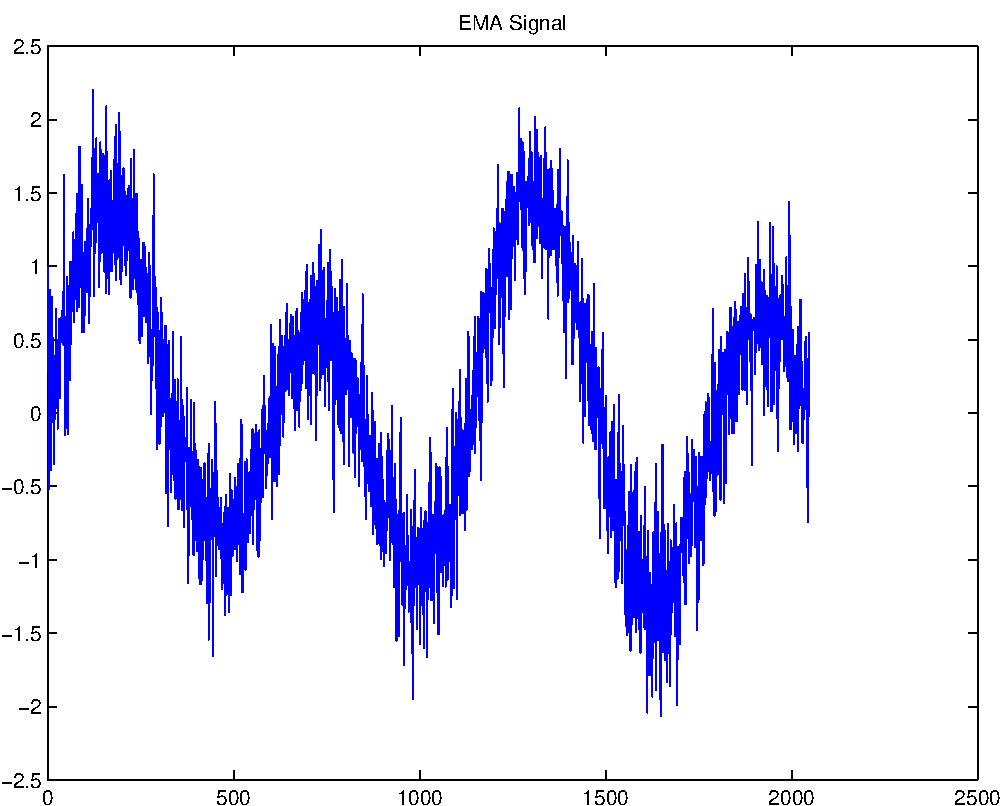
\includegraphics[width=10.0cm,height=10.0cm]{EMA_signal.pdf}

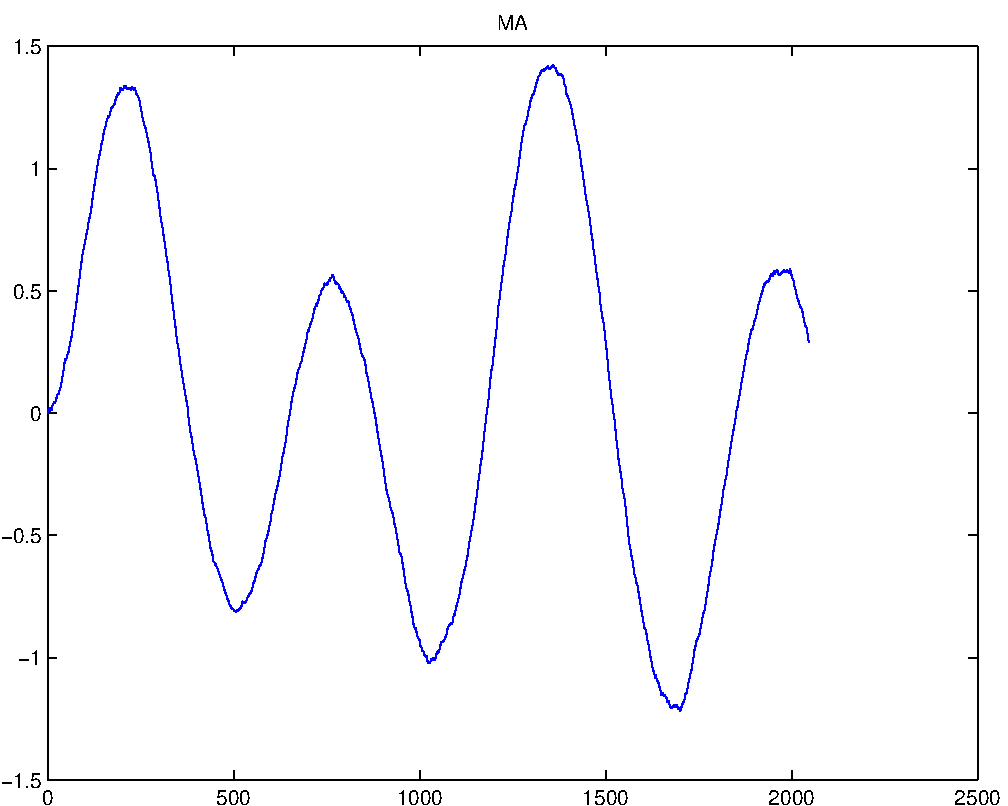
\includegraphics[width=10.0cm,height=10.0cm]{MA.pdf}

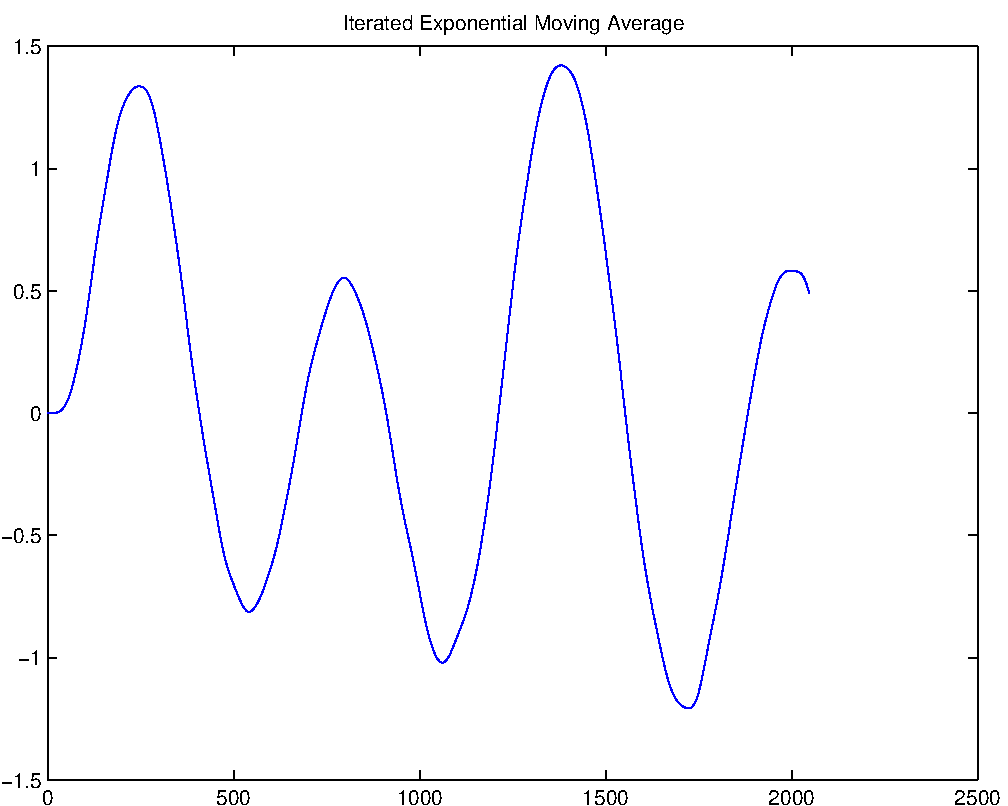
\includegraphics[width=10.0cm,height=10.0cm]{IEMA.pdf}

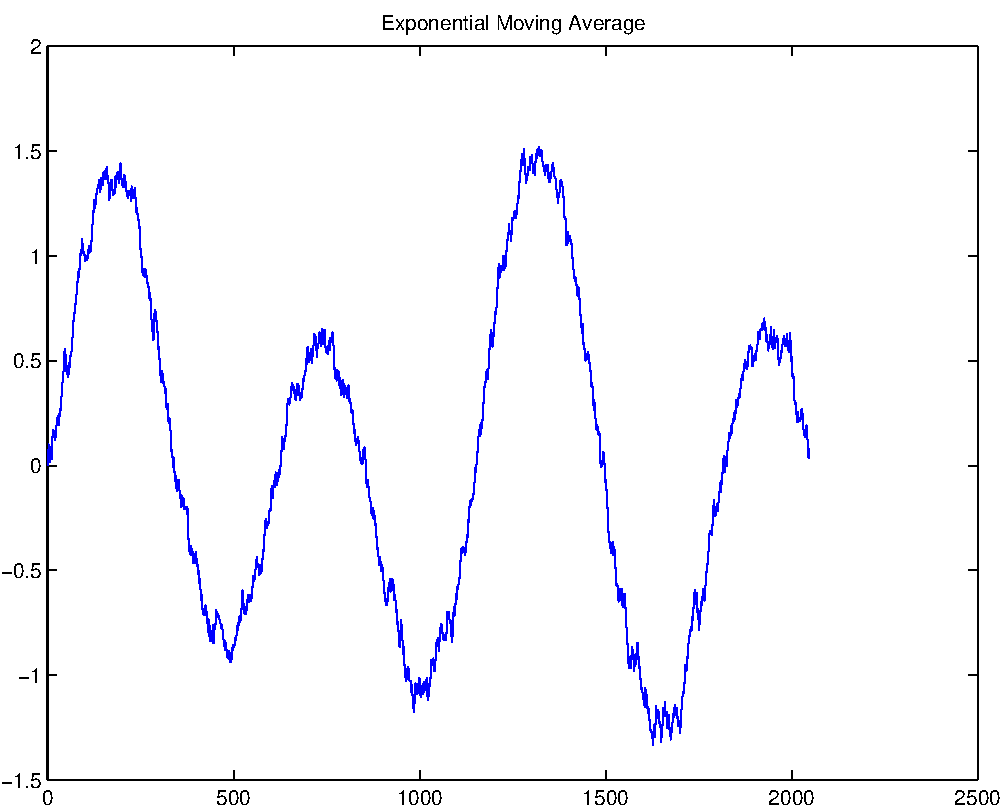
\includegraphics[width=10.0cm,height=10.0cm]{EMA.pdf}

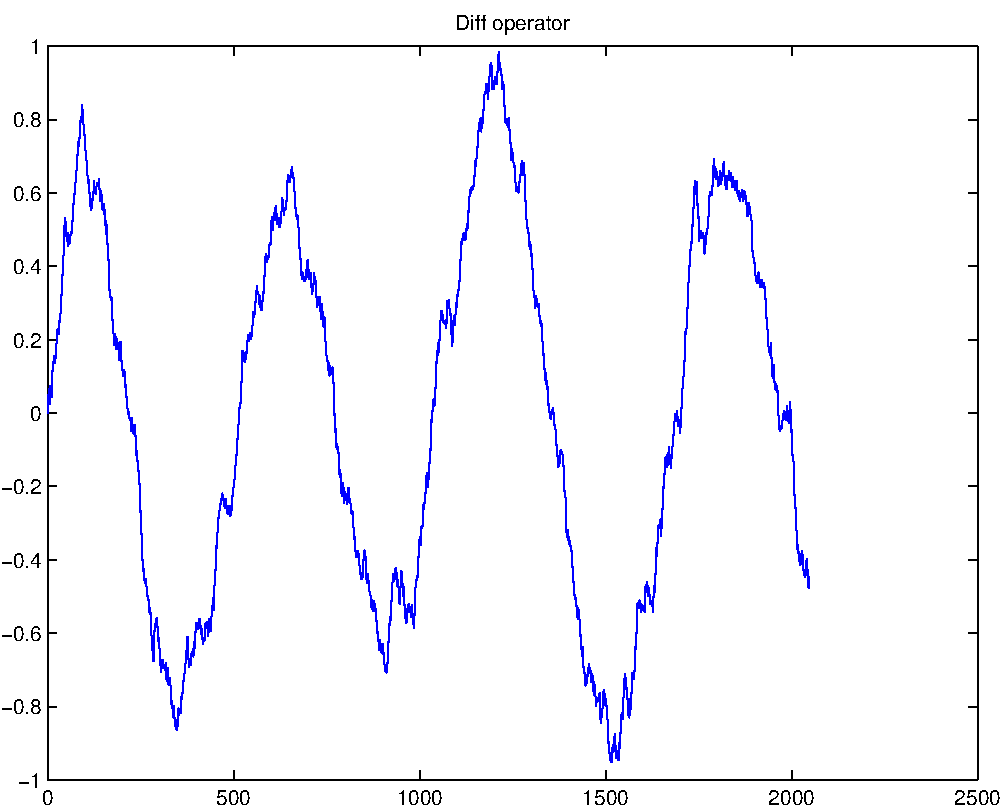
\includegraphics[width=10.0cm,height=10.0cm]{DIFF.pdf}

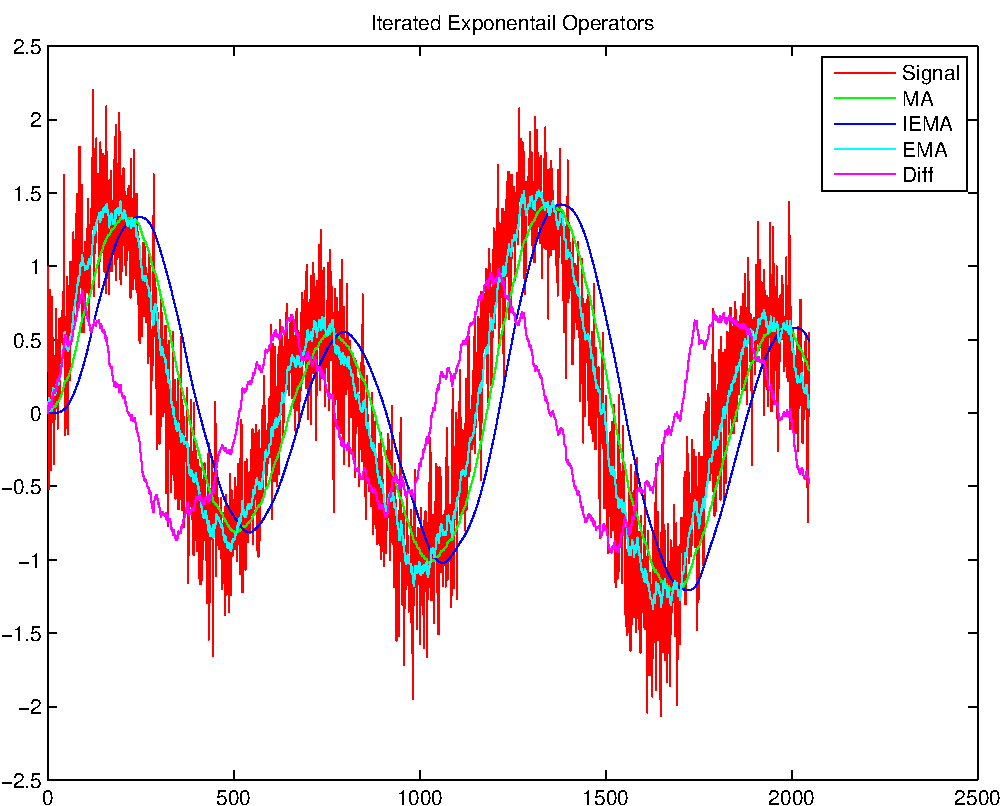
\includegraphics[width=10.0cm,height=10.0cm]{IteratedExponentailOperators.pdf}

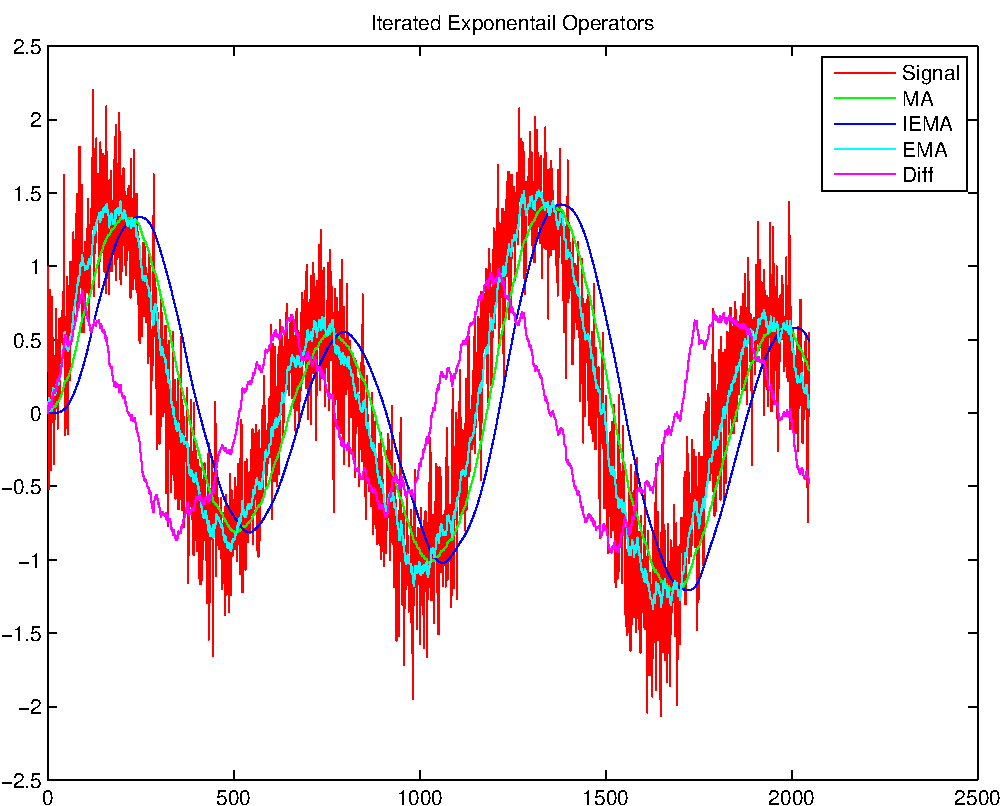
\includegraphics[width=10.0cm,height=10.0cm]{IteratedExponentailOperators.pdf}

QueryPerformanceCounter  =  +8.134
\subsubsection{Testing binary writer}
Binary writer Speedup 1GB Double Matrix +63.144

Binary reader Speedup 1GB Double Matrix +195.705

Binary writer Speedup 1GB Double vector +10.109

Binary reader Speedup 1GB Double Matrix +201.560

QueryPerformanceCounter  =  +1.026
\subsubsection{Testing Gaussian Mixture Point Cloud and Latex Plotting Capabilities.}
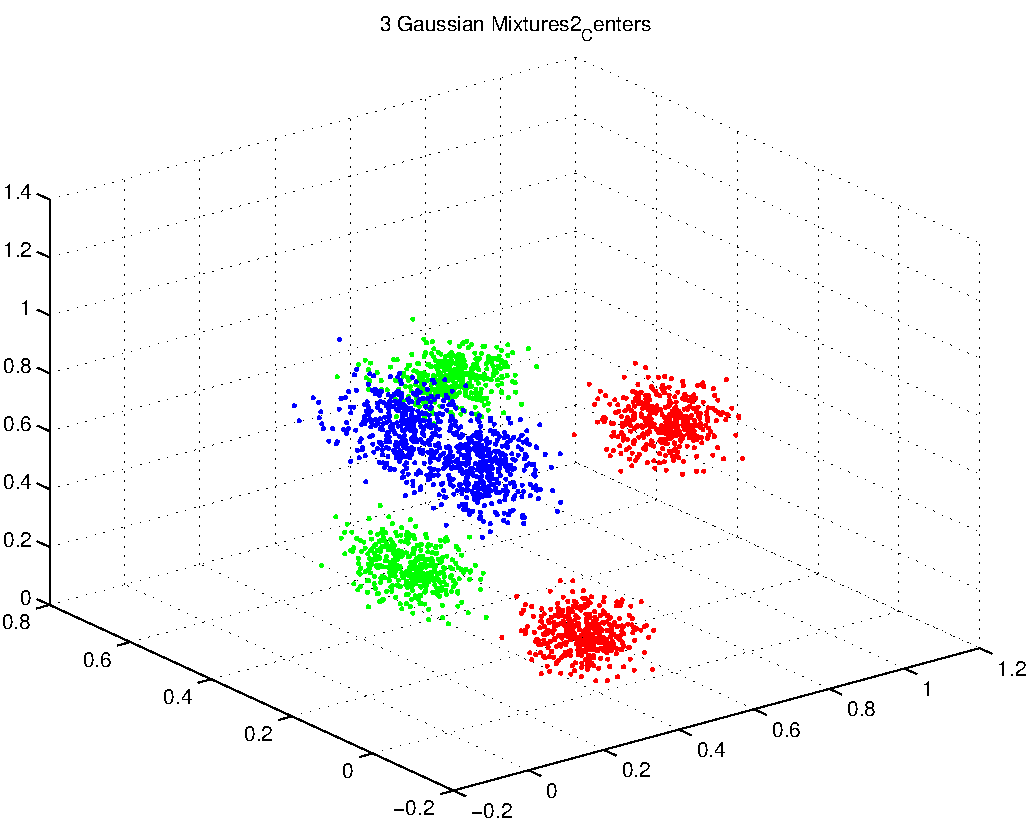
\includegraphics[width=10.0cm,height=10.0cm]{GaussianMixture_Dim_3_Centers2.pdf}

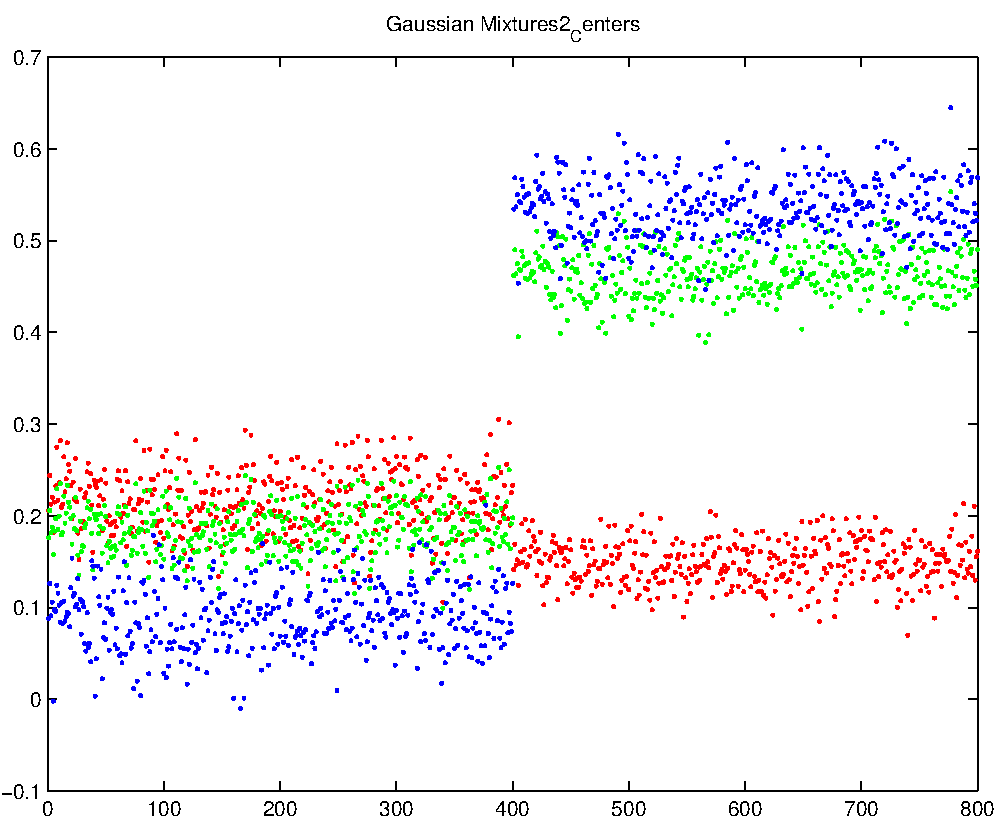
\includegraphics[width=10.0cm,height=10.0cm]{GaussianMixture_Dim_1_Centers2.pdf}

QueryPerformanceCounter  =  +2.906
\subsubsection{Intel VSL Function Check}
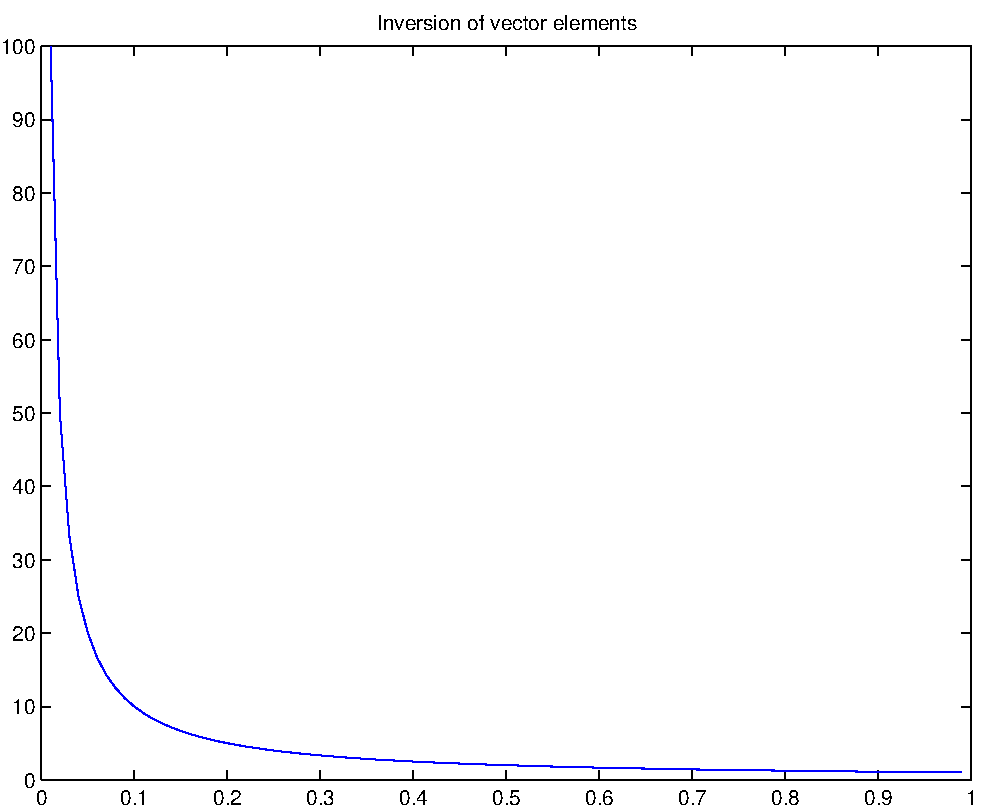
\includegraphics[width=10.0cm,height=10.0cm]{klVSLInv.pdf}

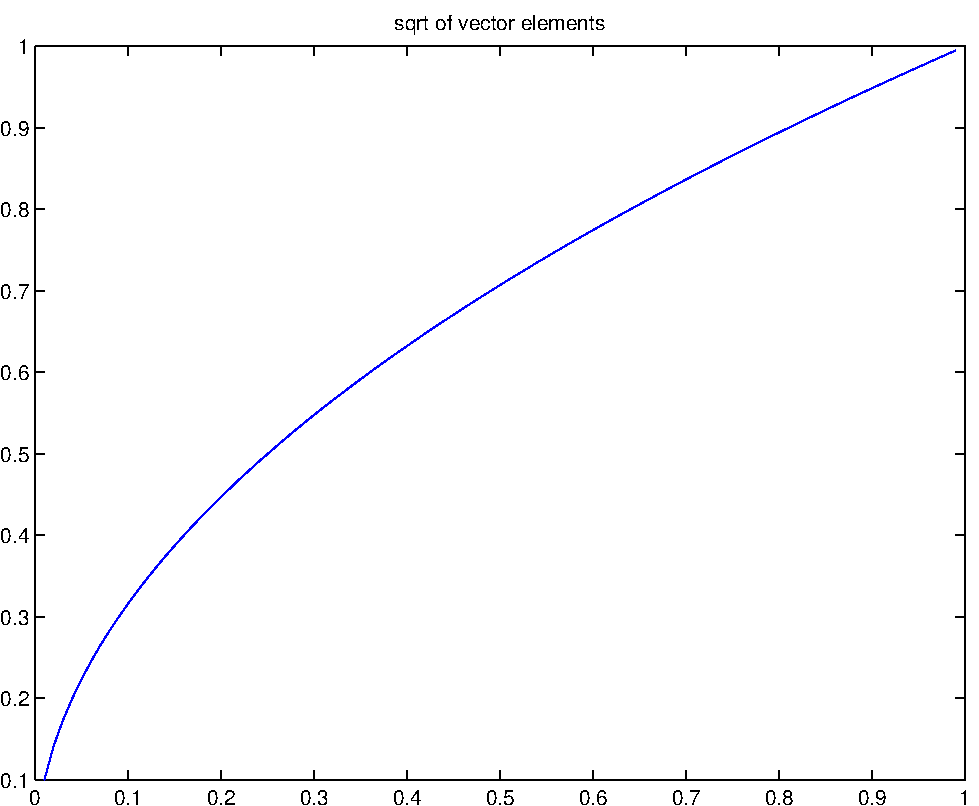
\includegraphics[width=10.0cm,height=10.0cm]{klVSLSqrt.pdf}

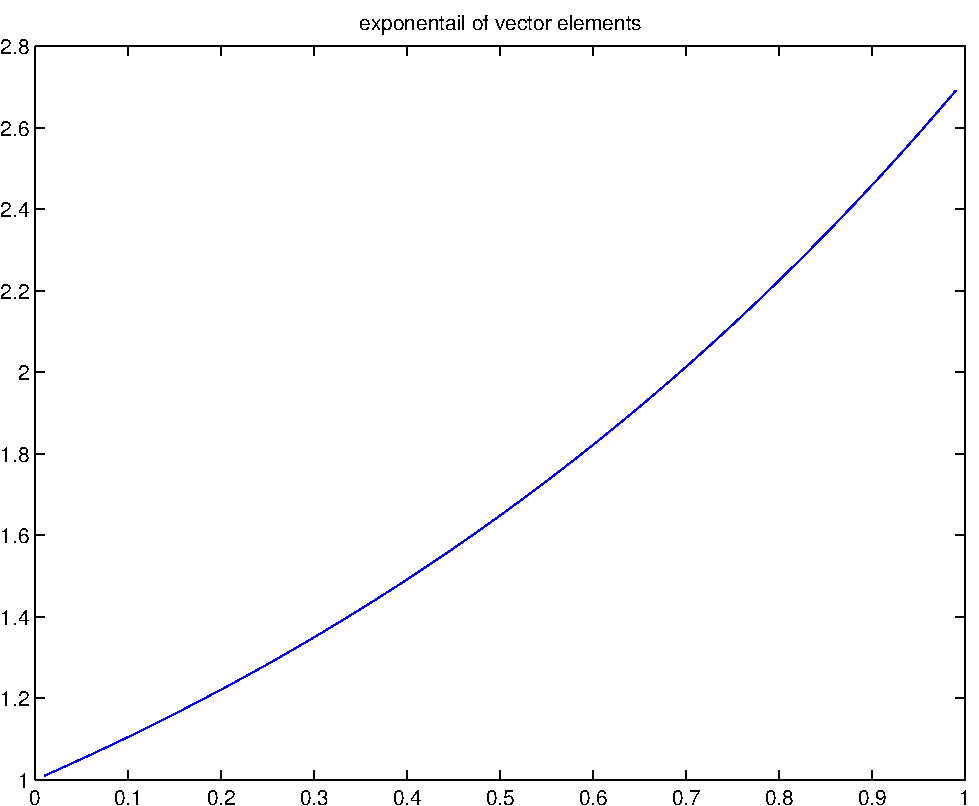
\includegraphics[width=10.0cm,height=10.0cm]{klVSLExp.pdf}

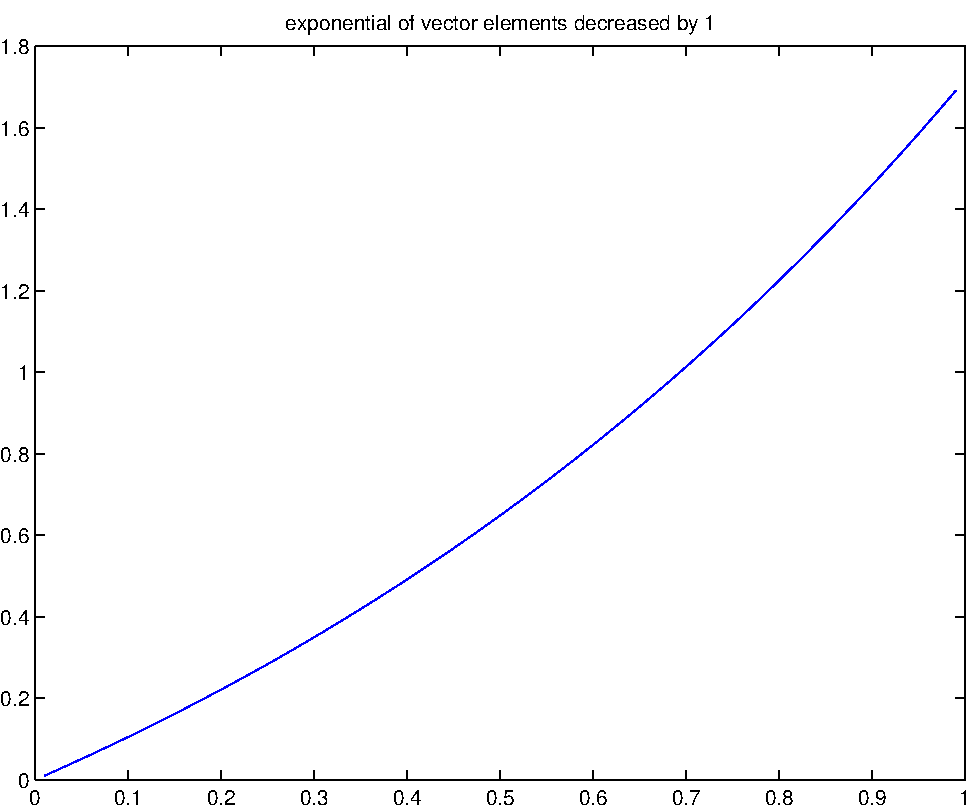
\includegraphics[width=10.0cm,height=10.0cm]{klVSLExpm1.pdf}

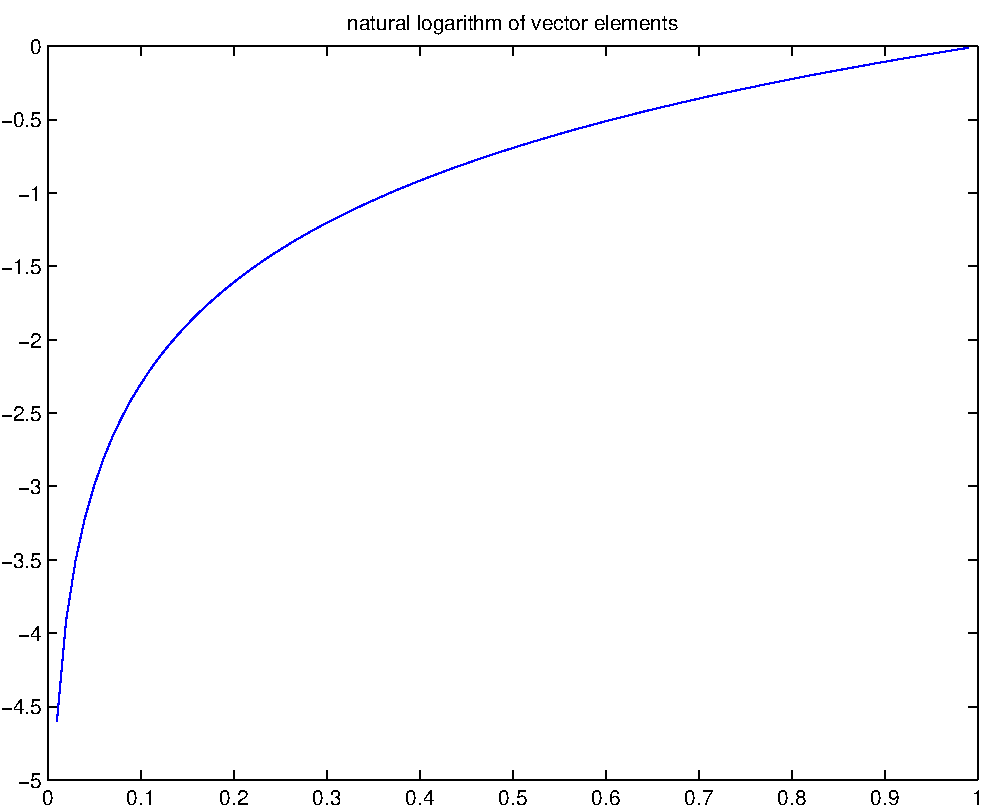
\includegraphics[width=10.0cm,height=10.0cm]{klVSLLn.pdf}

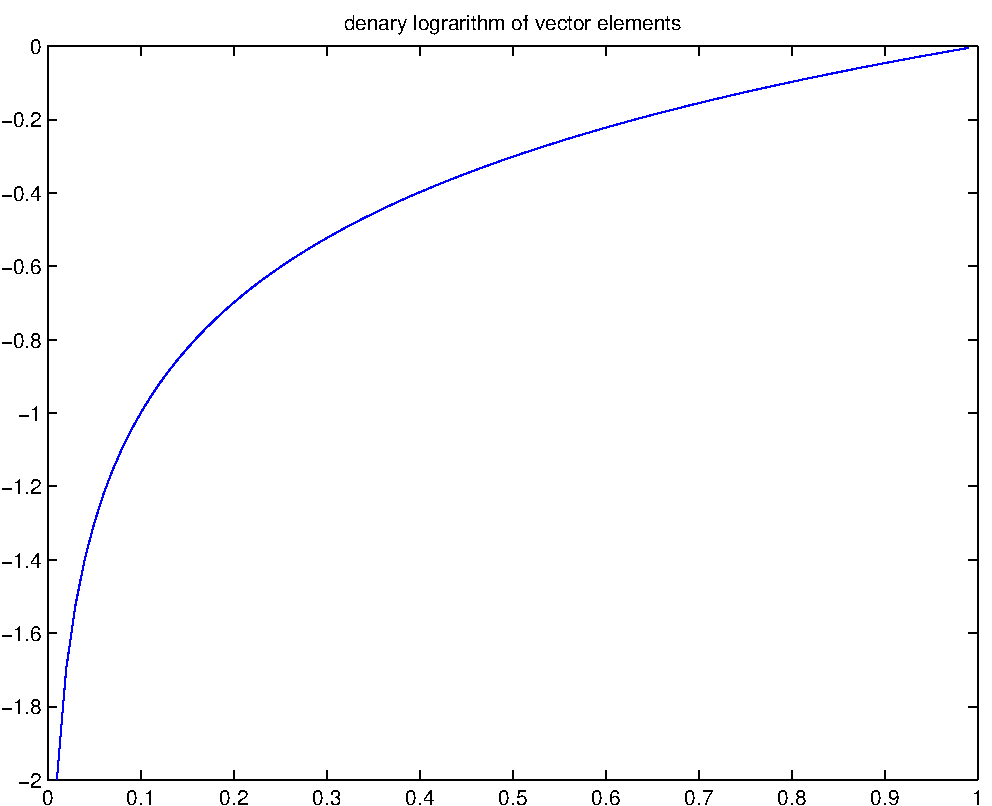
\includegraphics[width=10.0cm,height=10.0cm]{klVSLLog10.pdf}

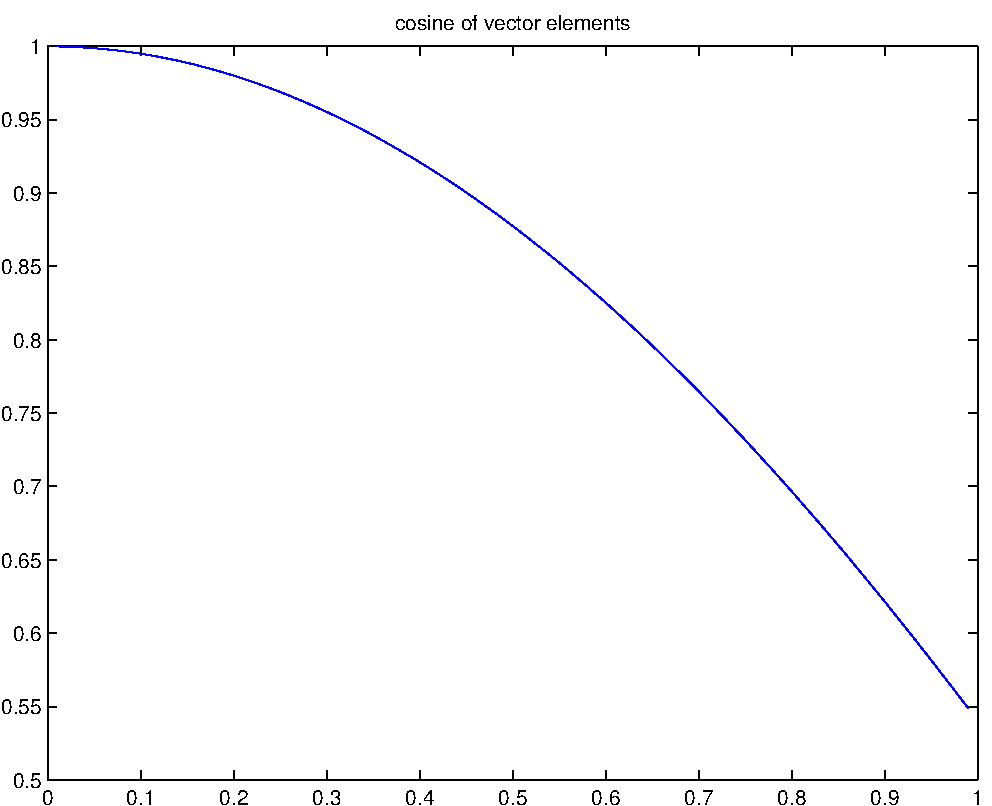
\includegraphics[width=10.0cm,height=10.0cm]{klVSLCos.pdf}

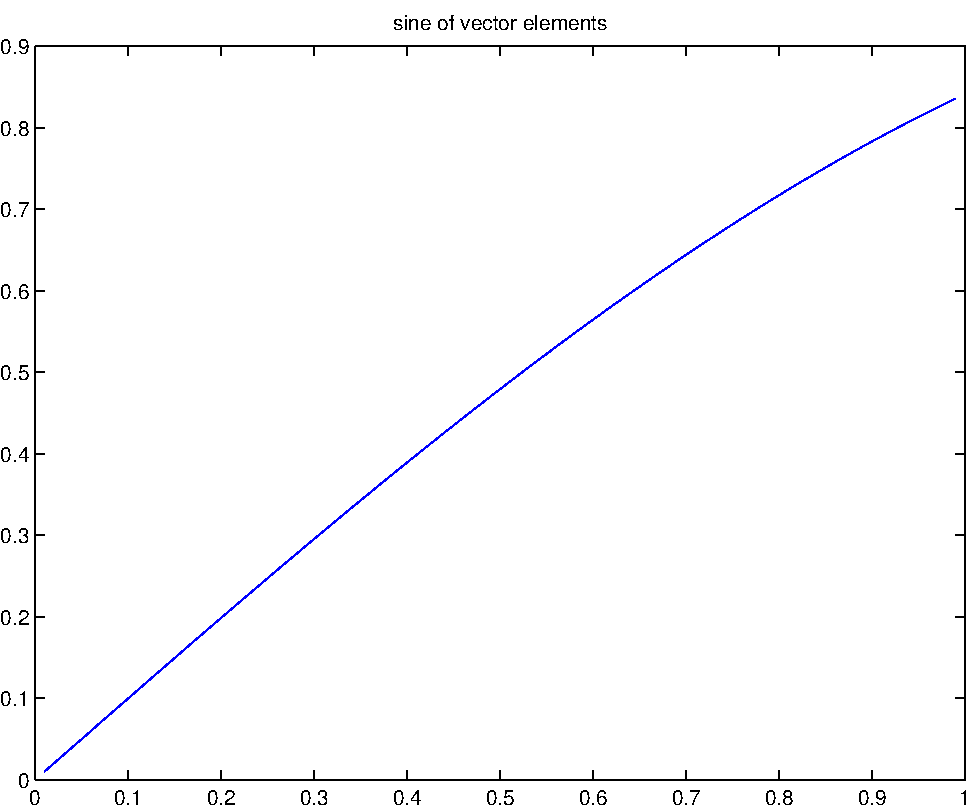
\includegraphics[width=10.0cm,height=10.0cm]{klVSLSin.pdf}

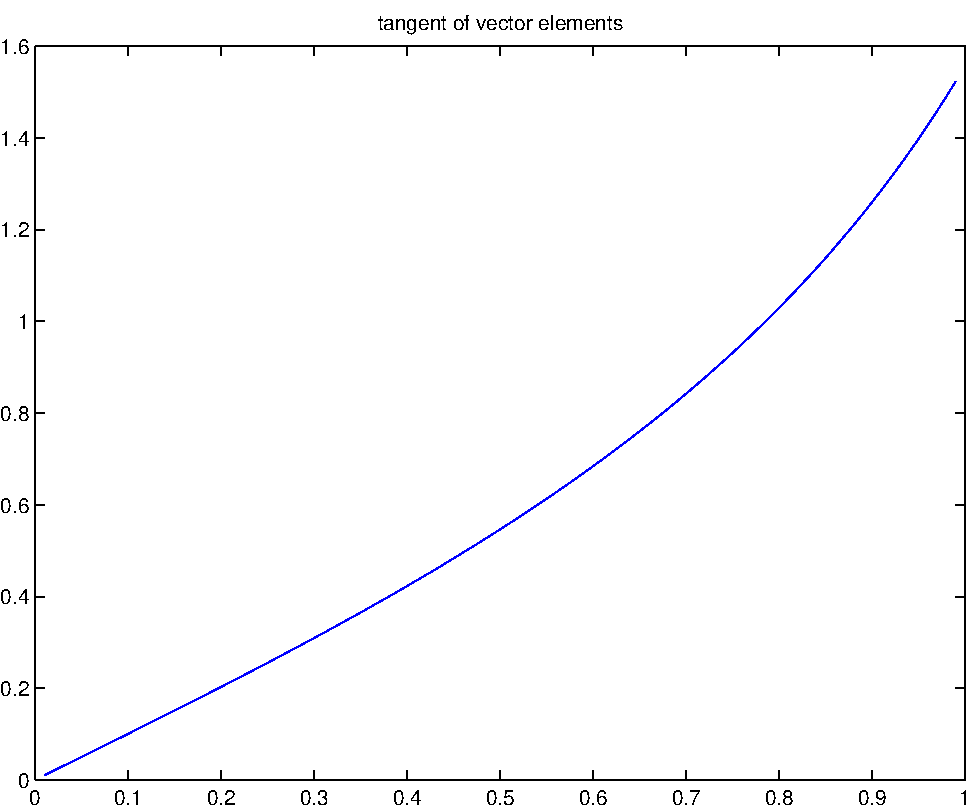
\includegraphics[width=10.0cm,height=10.0cm]{klVSLTan.pdf}

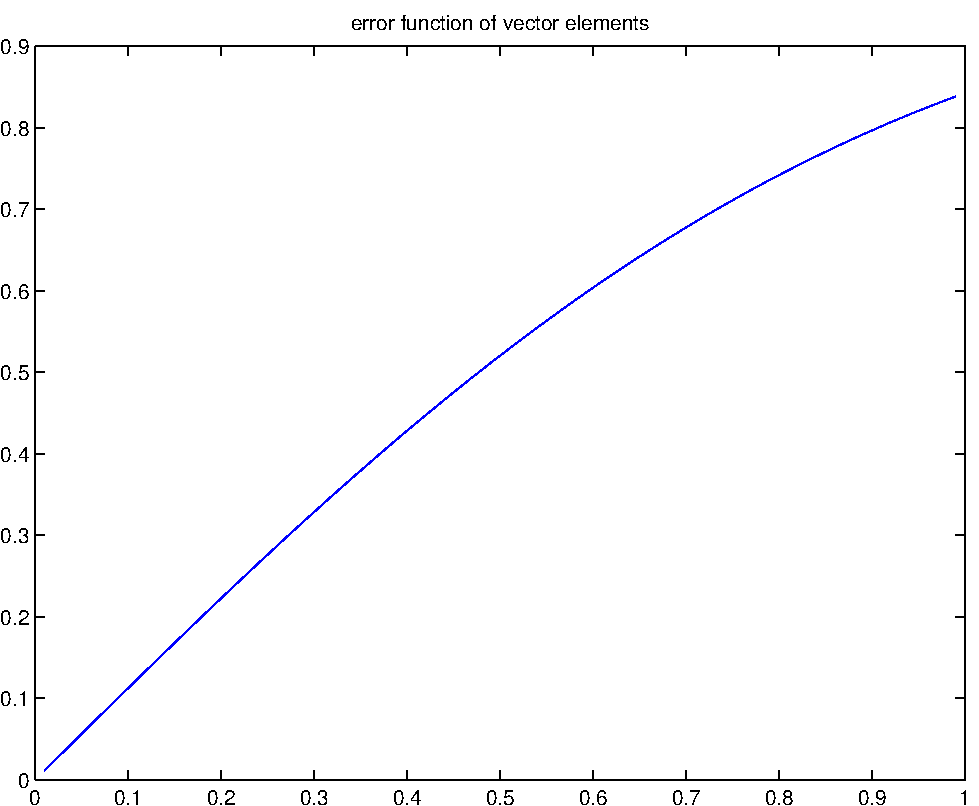
\includegraphics[width=10.0cm,height=10.0cm]{klVSLErf.pdf}

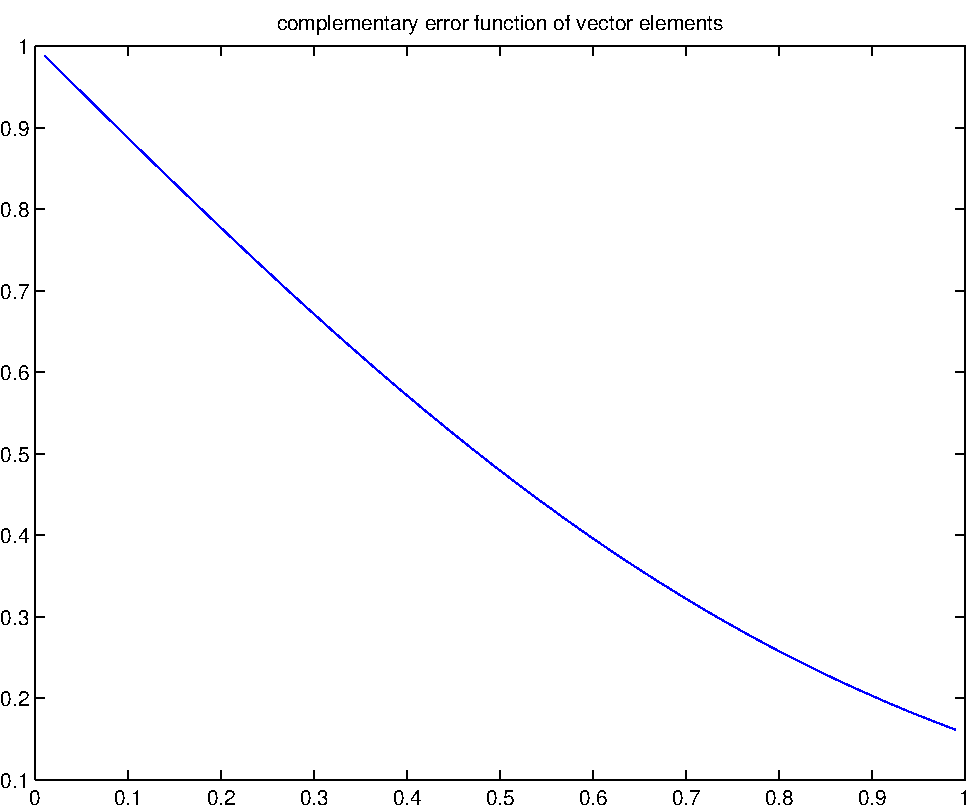
\includegraphics[width=10.0cm,height=10.0cm]{klVSLErfc.pdf}

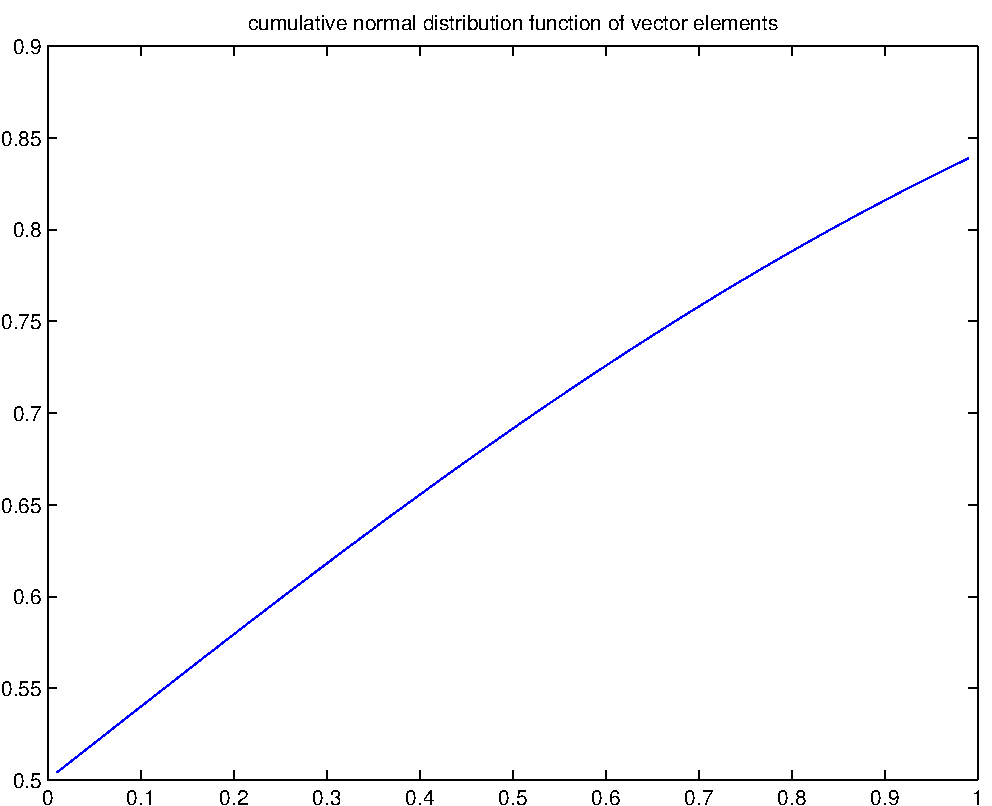
\includegraphics[width=10.0cm,height=10.0cm]{klVSLCdfNorm.pdf}

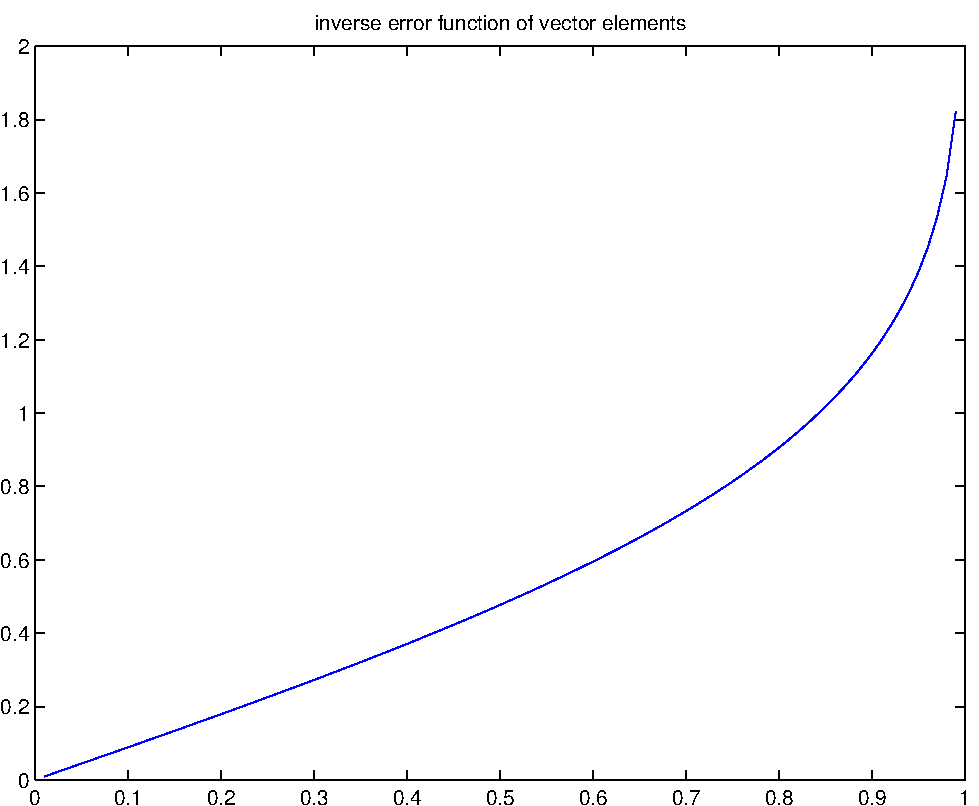
\includegraphics[width=10.0cm,height=10.0cm]{klVSLErfInv.pdf}

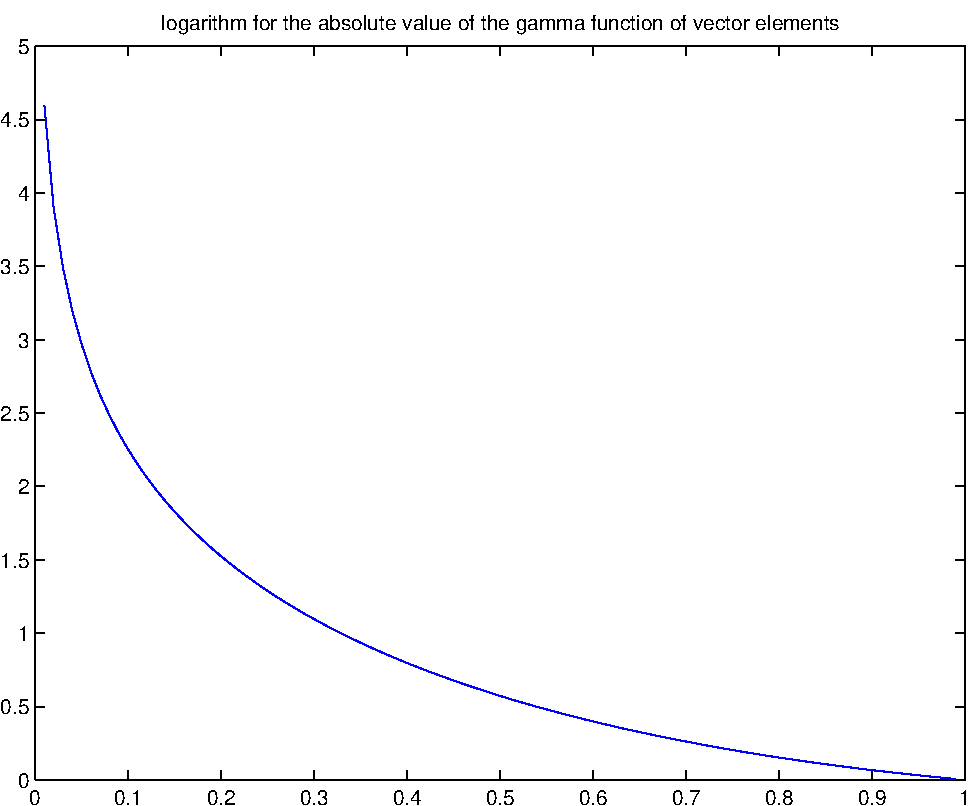
\includegraphics[width=10.0cm,height=10.0cm]{klVSLLGamma.pdf}

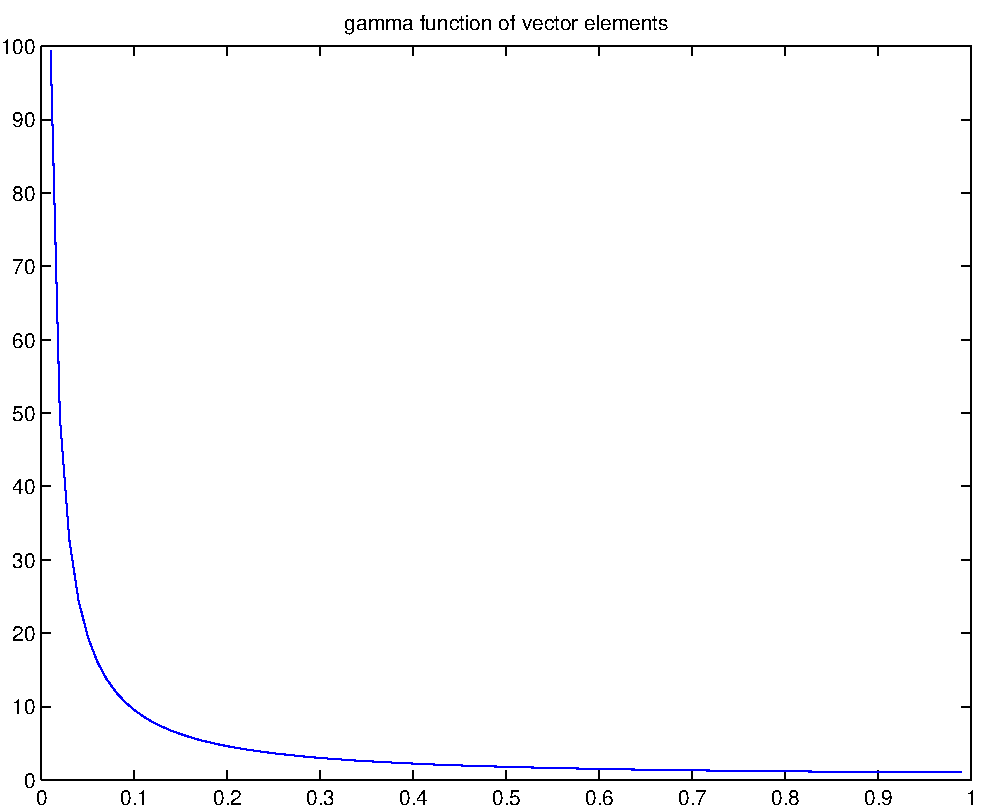
\includegraphics[width=10.0cm,height=10.0cm]{klVSLTGamma.pdf}

QueryPerformanceCounter  =  +15.665
\subsubsection{Gram Matrix Consistency Check}
Sample Size = 4096
Feature dim = 3

$$Sigma$ = \left(
\begin{array}{
ccc}
+1.140 & +1.535 & +0.581 \\
+1.535 & +9.988 & +1.605 \\
+0.581 & +1.605 & +0.428 \\
\end{array}
\right)$ \newline 

$Sample Covariance = \left(
\begin{array}{
ccc}
+1.153 & +1.656 & +0.591 \\
+1.656 & +10.198 & +1.681 \\
+0.591 & +1.681 & +0.437 \\
\end{array}
\right)$ \newline 

$Sample Mean = \left(
\begin{array}{
ccc}
+1.02688 & +1.08012 & +1.01670 \\
\end{array}
\right)$ \newline 

$Sample Covariance-$Omega$ = \left(
\begin{array}{
ccc}
+0.013 & +0.121 & +0.010 \\
+0.121 & +0.209 & +0.076 \\
+0.010 & +0.076 & +0.009 \\
\end{array}
\right)$ \newline 

$Sample Covariance Eigs = \left(
\begin{array}{
ccc}
(+10.79008,+0.00000) & (+0.95798,+0.00000) & (+0.03928,+0.00000) \\
\end{array}
\right)$ \newline 

$Centered Mean = \left(
\begin{array}{
ccc}
+0.00000 & -0.00000 & +0.00000 \\
\end{array}
\right)$ \newline 

$Centered Covariance = \left(
\begin{array}{
ccc}
+1.153 & +1.656 & +0.591 \\
+1.656 & +10.198 & +1.681 \\
+0.591 & +1.681 & +0.437 \\
\end{array}
\right)$ \newline 

$Gram Matrix Gf Not scaled by sample size = \left(
\begin{array}{
ccc}
+4723.612 & +6780.059 & +2420.098 \\
+6780.059 & +41769.171 & +6884.815 \\
+2420.098 & +6884.815 & +1788.187 \\
\end{array}
\right)$ \newline 

$Gram Matrix Gf  scaled by sample size = \left(
\begin{array}{
ccc}
+1.153 & +1.655 & +0.591 \\
+1.655 & +10.198 & +1.681 \\
+0.591 & +1.681 & +0.437 \\
\end{array}
\right)$ \newline 

$SampleCovariance - Scaled Gf = \left(
\begin{array}{
ccc}
+0.000 & +0.000 & +0.000 \\
+0.000 & +0.002 & +0.000 \\
+0.000 & +0.000 & +0.000 \\
\end{array}
\right)$ \newline 

$EigenDecomp of SampleCovariance = \left(
\begin{array}{
ccc}
-0.177 & -0.970 & -0.168 \\
+0.920 & -0.223 & +0.322 \\
-0.350 & -0.097 & +0.932 \\
\end{array}
\right)$ \newline 

$EigenDecomp of Gram Matrix = \left(
\begin{array}{
ccc}
-0.131 & -0.972 & -0.194 \\
-0.362 & +0.229 & -0.903 \\
+0.923 & -0.048 & -0.382 \\
\end{array}
\right)$ \newline 

QueryPerformanceCounter  =  +1.416
\subsubsection{Eigen Solver Checks}
\subsubsection{Haar Distributed Random Orthogonal Matrix $A \in O(n)$}
 Testing Operator Norm
Number of Dimensions: +8

$A = \left(
\begin{array}{
cccccccc}
-0.024 & +0.193 & -0.083 & -0.583 & +0.760 & -0.115 & -0.086 & +0.130 \\
+0.409 & -0.023 & -0.263 & -0.536 & -0.324 & -0.149 & +0.428 & -0.407 \\
+0.110 & -0.558 & -0.646 & +0.165 & +0.106 & -0.340 & -0.319 & +0.048 \\
+0.449 & +0.186 & +0.029 & +0.523 & +0.470 & -0.010 & +0.131 & -0.501 \\
+0.322 & +0.590 & -0.023 & +0.085 & -0.245 & -0.558 & -0.272 & +0.306 \\
+0.075 & +0.399 & -0.633 & +0.062 & -0.057 & +0.630 & -0.023 & +0.171 \\
-0.555 & +0.295 & -0.174 & -0.051 & -0.103 & -0.140 & -0.362 & -0.641 \\
-0.448 & +0.144 & -0.271 & +0.243 & +0.103 & -0.347 & +0.696 & +0.175 \\
\end{array}
\right)$ \newline 

$Det(A) :   A \in O(n)$ = (-1.000,-0.000)

$L = \left(
\begin{array}{
cccccccc}
+1.000 & +0.000 & +0.000 & +0.000 & +0.000 & +0.000 & +0.000 & +0.000 \\
-0.581 & +1.000 & +0.000 & +0.000 & +0.000 & +0.000 & +0.000 & +0.000 \\
-0.198 & -0.657 & +1.000 & +0.000 & +0.000 & +0.000 & +0.000 & +0.000 \\
-0.736 & +0.255 & +0.472 & +1.000 & +0.000 & +0.000 & +0.000 & +0.000 \\
+0.044 & +0.237 & +0.060 & +0.893 & +1.000 & +0.000 & +0.000 & +0.000 \\
-0.135 & +0.576 & +0.768 & +0.182 & +0.223 & +1.000 & +0.000 & +0.000 \\
+0.806 & -0.123 & +0.190 & -0.376 & +0.064 & -0.029 & +1.000 & +0.000 \\
-0.810 & +0.558 & +0.056 & -0.650 & +0.359 & +0.331 & +0.349 & +1.000 \\
\end{array}
\right)$ \newline 

$U = \left(
\begin{array}{
cccccccc}
-0.555 & +0.295 & -0.174 & -0.051 & -0.103 & -0.140 & -0.362 & -0.641 \\
+0.000 & +0.762 & -0.124 & +0.055 & -0.305 & -0.639 & -0.482 & -0.066 \\
+0.000 & +0.000 & -0.762 & +0.191 & -0.115 & -0.788 & -0.708 & -0.123 \\
+0.000 & +0.000 & +0.000 & -0.678 & -0.269 & +0.282 & +0.619 & -0.804 \\
+0.000 & +0.000 & +0.000 & +0.000 & +1.084 & -0.162 & -0.466 & +0.899 \\
+0.000 & +0.000 & +0.000 & +0.000 & +0.000 & +1.570 & +0.741 & +0.162 \\
+0.000 & +0.000 & +0.000 & +0.000 & +0.000 & +0.000 & +1.348 & +0.351 \\
+0.000 & +0.000 & +0.000 & +0.000 & +0.000 & +0.000 & +0.000 & -1.997 \\
\end{array}
\right)$ \newline 

$L * U  = \left(
\begin{array}{
cccccccc}
-0.555 & +0.295 & -0.174 & -0.051 & -0.103 & -0.140 & -0.362 & -0.641 \\
+0.322 & +0.590 & -0.023 & +0.085 & -0.245 & -0.558 & -0.272 & +0.306 \\
+0.110 & -0.558 & -0.646 & +0.165 & +0.106 & -0.340 & -0.319 & +0.048 \\
+0.409 & -0.023 & -0.263 & -0.536 & -0.324 & -0.149 & +0.428 & -0.407 \\
-0.024 & +0.193 & -0.083 & -0.583 & +0.760 & -0.115 & -0.086 & +0.130 \\
+0.075 & +0.399 & -0.633 & +0.062 & -0.057 & +0.630 & -0.023 & +0.171 \\
-0.448 & +0.144 & -0.271 & +0.243 & +0.103 & -0.347 & +0.696 & +0.175 \\
+0.449 & +0.186 & +0.029 & +0.523 & +0.470 & -0.010 & +0.131 & -0.501 \\
\end{array}
\right)$ \newline 

$Det(L) :    = (+1.000,+0.000)     Det(U) :    = (+1.000,+0.000)     Det(LU) :    = (+1.000,+0.000)$

$||A||_{L_1}$  = +2.393

$||A||_{L_{\infty}}$ = +2.539

$||A^{-1}||_{L_1}$  = +2.539

$||A^{-1}||_{L_{\infty}}$ = +2.393

$||A||_{L_{\infty}} * ||A^{-1}||_{L_{\infty}} = +6.075$

$||A||_{L_1} * ||A^{-1}||_{L_1} = +6.075$

Frobenious Norm  $||A||_{\textit{F}}$ via $\sum\limits_{i,j =0}^{n} \|A_{i,j}|$   of  $A \in O(n)$  +2.828

$L_1$ condition number of Haar Distributed Random Orthogonal Matrix $A \in O(n)$ +6.075

$A = \left(
\begin{array}{
cccccccc}
-0.024 & +0.193 & -0.083 & -0.583 & +0.760 & -0.115 & -0.086 & +0.130 \\
+0.409 & -0.023 & -0.263 & -0.536 & -0.324 & -0.149 & +0.428 & -0.407 \\
+0.110 & -0.558 & -0.646 & +0.165 & +0.106 & -0.340 & -0.319 & +0.048 \\
+0.449 & +0.186 & +0.029 & +0.523 & +0.470 & -0.010 & +0.131 & -0.501 \\
+0.322 & +0.590 & -0.023 & +0.085 & -0.245 & -0.558 & -0.272 & +0.306 \\
+0.075 & +0.399 & -0.633 & +0.062 & -0.057 & +0.630 & -0.023 & +0.171 \\
-0.555 & +0.295 & -0.174 & -0.051 & -0.103 & -0.140 & -0.362 & -0.641 \\
-0.448 & +0.144 & -0.271 & +0.243 & +0.103 & -0.347 & +0.696 & +0.175 \\
\end{array}
\right)$ \newline 

$L_{\infty}$ condition number of Haar Distributed Random Orthogonal Matrix $A \in O(n)$ +6.068

Eigenvalues of $A \in O(n)$

(+0.625,+0.780), (+0.625,-0.780), (+0.232,+0.973), (+0.232,-0.973), (-0.844,+0.537), (-0.844,-0.537), (-1.000,+0.000), (+1.000,+0.000)

 $|\lambda | : \lambda \in \sigma(A) , A \in O(n)$

+1.000, +1.000, +1.000, +1.000, +1.000, +1.000, +1.000, +1.000


Calculating $A^{\dag} A,$  we expect $A^{\dag} A \approx I$

$A^{\dag} A = \left(
\begin{array}{
cccccccc}
+1.000 & +0.000 & +0.000 & +0.000 & -0.000 & +0.000 & +0.000 & -0.000 \\
+0.000 & +1.000 & +0.000 & -0.000 & -0.000 & -0.000 & -0.000 & -0.000 \\
+0.000 & +0.000 & +1.000 & -0.000 & -0.000 & +0.000 & +0.000 & +0.000 \\
+0.000 & -0.000 & -0.000 & +1.000 & +0.000 & +0.000 & +0.000 & +0.000 \\
-0.000 & -0.000 & -0.000 & +0.000 & +1.000 & +0.000 & +0.000 & +0.000 \\
+0.000 & -0.000 & +0.000 & +0.000 & +0.000 & +1.000 & +0.000 & -0.000 \\
+0.000 & -0.000 & +0.000 & +0.000 & +0.000 & +0.000 & +1.000 & +0.000 \\
-0.000 & -0.000 & +0.000 & +0.000 & +0.000 & -0.000 & +0.000 & +1.000 \\
\end{array}
\right)$ \newline 

Calculating $A^{-1} ,  A \in O(n)$.

$A^{-1} = \left(
\begin{array}{
cccccccc}
-0.024 & +0.409 & +0.110 & +0.449 & +0.322 & +0.075 & -0.555 & -0.448 \\
+0.193 & -0.023 & -0.558 & +0.186 & +0.590 & +0.399 & +0.295 & +0.144 \\
-0.083 & -0.263 & -0.646 & +0.029 & -0.023 & -0.633 & -0.174 & -0.271 \\
-0.583 & -0.536 & +0.165 & +0.523 & +0.085 & +0.062 & -0.051 & +0.243 \\
+0.760 & -0.324 & +0.106 & +0.470 & -0.245 & -0.057 & -0.103 & +0.103 \\
-0.115 & -0.149 & -0.340 & -0.010 & -0.558 & +0.630 & -0.140 & -0.347 \\
-0.086 & +0.428 & -0.319 & +0.131 & -0.272 & -0.023 & -0.362 & +0.696 \\
+0.130 & -0.407 & +0.048 & -0.501 & +0.306 & +0.171 & -0.641 & +0.175 \\
\end{array}
\right)$ \newline 

Calculating $A^{-1} *A  ,  A \in O(n)$.   We expect $A^{-1} *A  \approx I$. 

$A^{-1} *A = \left(
\begin{array}{
cccccccc}
+1.000 & -0.000 & +0.000 & +0.000 & +0.000 & +0.000 & +0.000 & +0.000 \\
-0.000 & +1.000 & +0.000 & +0.000 & -0.000 & +0.000 & -0.000 & +0.000 \\
+0.000 & +0.000 & +1.000 & +0.000 & -0.000 & +0.000 & -0.000 & +0.000 \\
-0.000 & +0.000 & -0.000 & +1.000 & -0.000 & +0.000 & +0.000 & -0.000 \\
-0.000 & +0.000 & -0.000 & +0.000 & +1.000 & -0.000 & -0.000 & +0.000 \\
+0.000 & -0.000 & -0.000 & +0.000 & -0.000 & +1.000 & +0.000 & +0.000 \\
+0.000 & -0.000 & +0.000 & +0.000 & +0.000 & +0.000 & +1.000 & +0.000 \\
+0.000 & +0.000 & -0.000 & -0.000 & -0.000 & -0.000 & -0.000 & +1.000 \\
\end{array}
\right)$ \newline 

Calculating SVD of  $A \in O(n)$

$U = \left(
\begin{array}{
cccccccc}
-0.927 & +0.013 & +0.210 & +0.104 & +0.028 & +0.076 & -0.236 & +0.154 \\
+0.022 & -0.641 & +0.013 & -0.382 & -0.260 & -0.224 & -0.012 & +0.569 \\
-0.106 & +0.290 & -0.615 & -0.366 & -0.453 & -0.015 & -0.414 & -0.123 \\
+0.014 & +0.499 & +0.074 & +0.207 & -0.121 & -0.742 & +0.107 & +0.354 \\
-0.024 & +0.193 & -0.083 & -0.583 & +0.760 & -0.115 & -0.086 & +0.130 \\
-0.139 & +0.228 & -0.376 & +0.005 & -0.037 & +0.422 & +0.645 & +0.437 \\
+0.330 & +0.244 & +0.187 & +0.182 & +0.017 & +0.417 & -0.545 & +0.541 \\
-0.020 & -0.326 & -0.624 & +0.541 & +0.363 & -0.167 & -0.199 & +0.108 \\
\end{array}
\right)$ \newline 

$S = \left(
\begin{array}{
cccccccc}
+1.000 & +0.000 & +0.000 & +0.000 & +0.000 & +0.000 & +0.000 & +0.000 \\
+0.000 & +1.000 & +0.000 & +0.000 & +0.000 & +0.000 & +0.000 & +0.000 \\
+0.000 & +0.000 & +1.000 & +0.000 & +0.000 & +0.000 & +0.000 & +0.000 \\
+0.000 & +0.000 & +0.000 & +1.000 & +0.000 & +0.000 & +0.000 & +0.000 \\
+0.000 & +0.000 & +0.000 & +0.000 & +1.000 & +0.000 & +0.000 & +0.000 \\
+0.000 & +0.000 & +0.000 & +0.000 & +0.000 & +1.000 & +0.000 & +0.000 \\
+0.000 & +0.000 & +0.000 & +0.000 & +0.000 & +0.000 & +1.000 & +0.000 \\
+0.000 & +0.000 & +0.000 & +0.000 & +0.000 & +0.000 & +0.000 & +1.000 \\
\end{array}
\right)$ \newline 

$V = \left(
\begin{array}{
cccccccc}
+0.000 & +0.000 & +0.000 & -0.000 & +1.000 & +0.000 & +0.000 & -0.000 \\
-0.674 & +0.107 & +0.330 & -0.084 & +0.000 & +0.082 & -0.539 & -0.349 \\
-0.168 & +0.369 & +0.247 & -0.068 & +0.000 & -0.232 & -0.131 & +0.836 \\
-0.449 & -0.716 & -0.409 & -0.003 & +0.000 & -0.185 & -0.043 & +0.288 \\
-0.225 & -0.038 & +0.315 & +0.838 & +0.000 & -0.170 & +0.339 & -0.047 \\
-0.112 & -0.315 & +0.480 & -0.237 & +0.000 & +0.647 & +0.382 & +0.194 \\
+0.449 & -0.486 & +0.548 & -0.034 & +0.000 & -0.359 & -0.362 & -0.015 \\
+0.225 & -0.057 & -0.185 & +0.477 & +0.000 & +0.573 & -0.547 & +0.237 \\
\end{array}
\right)$ \newline 

$U S V = \left(
\begin{array}{
cccccccc}
-0.177 & +0.085 & -0.099 & +0.071 & -0.927 & +0.151 & +0.000 & +0.255 \\
+0.808 & +0.264 & -0.353 & +0.161 & +0.022 & +0.245 & -0.120 & +0.228 \\
-0.038 & +0.297 & -0.260 & -0.402 & -0.106 & +0.379 & -0.002 & -0.725 \\
-0.204 & +0.098 & -0.302 & +0.192 & +0.014 & -0.310 & -0.844 & -0.109 \\
-0.022 & +0.449 & +0.394 & +0.721 & -0.024 & +0.045 & +0.106 & -0.330 \\
+0.257 & -0.588 & +0.444 & +0.062 & -0.139 & +0.404 & -0.398 & -0.215 \\
-0.452 & +0.067 & -0.142 & +0.158 & +0.330 & +0.716 & -0.097 & +0.340 \\
-0.047 & -0.523 & -0.578 & +0.471 & -0.020 & -0.018 & +0.306 & -0.273 \\
\end{array}
\right)$ \newline 

Calculating first few eigenvectors of $A \in O(n)$ using LAPACK syevx

\subsubsection{Wishart Matrix $A \in W(n)$}
$L_1$ condition number of Wishart Matrix +1489.694
$L_infty$ condition number of Wishart Matrix +1489.694
\subsubsection{Gaussian Orthogonal Ensemble $A \in GOE(n)$}
$L_1$ condition number of GOE Matrix +66.900
$L_\infty$ condition number of GOE Matrix +66.900
\subsubsection{The Identity Matrix $I \in M(n)$}
$L_1$ condition number of $I$ = +1.000
$L_\infty$ condition number of $I$ = +1.000
QueryPerformanceCounter  =  +0.326
\subsubsection{Generate Tracey Widom Sample}
\subsubsection{Sample from $W_n m$ times and calculate empirical PDF of the first eig}
Here we generate histograms of $\lambda_1$ for GOE (Gaussian Orthogonal Ensemble), and W (Wishart) 		 distributed of random matrices
These should approximate the celebrated Tracy Widom distribution.
Dimension $n = +128$

Sample size $m = 32$

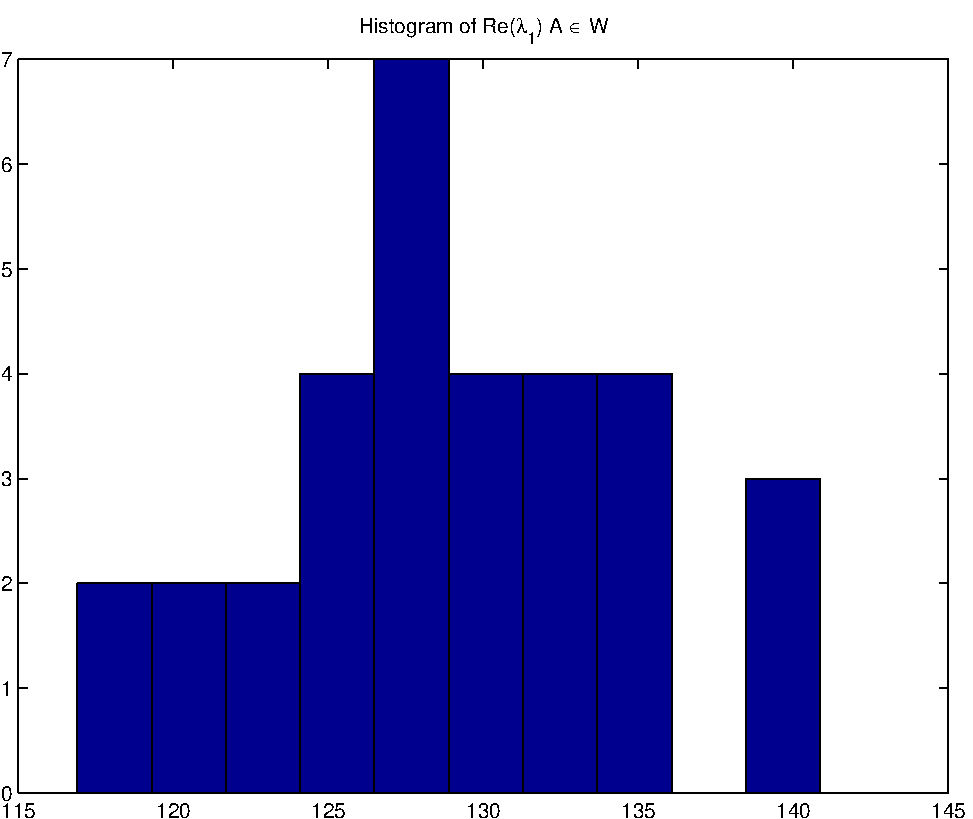
\includegraphics[width=10.0cm,height=10.0cm]{Re_TraceyWidom.pdf}

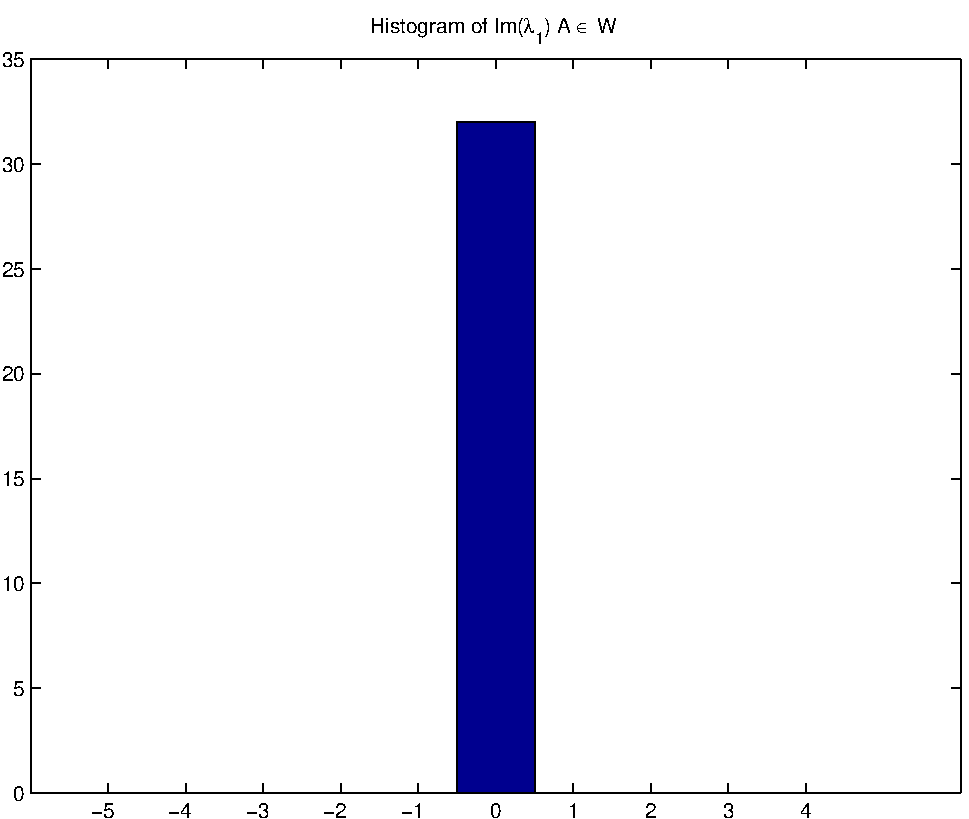
\includegraphics[width=10.0cm,height=10.0cm]{Im_TraceyWidom.pdf}

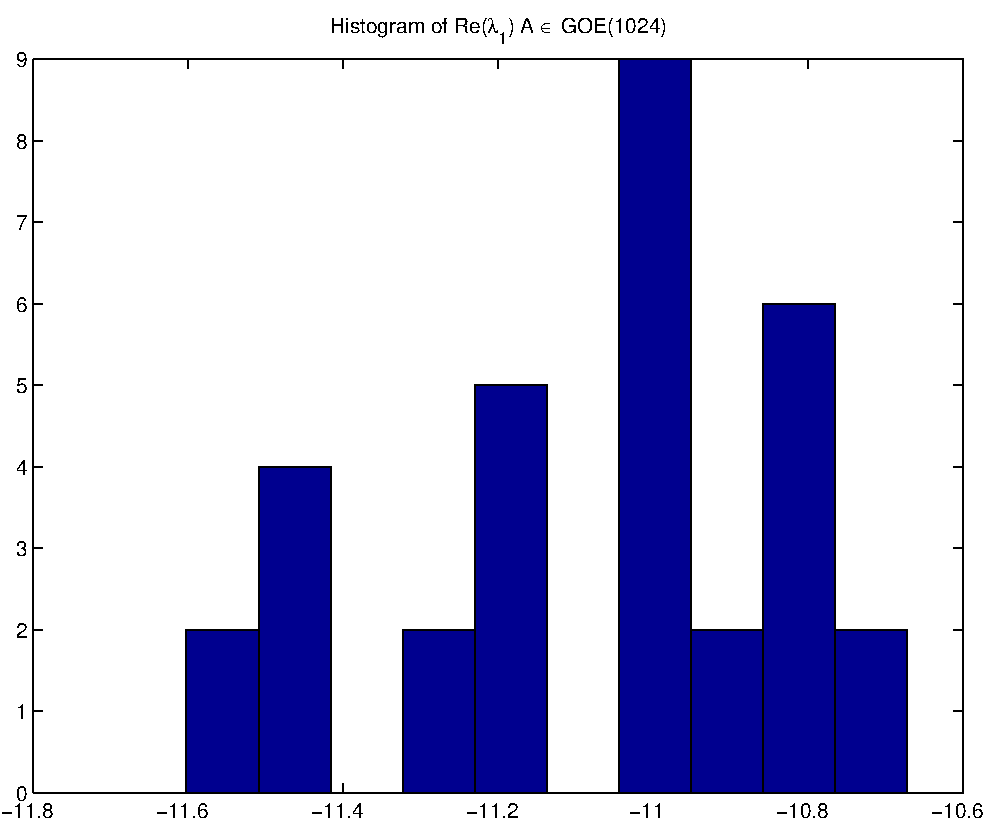
\includegraphics[width=10.0cm,height=10.0cm]{Re_Winger.pdf}

\includegraphics[width=10.0cm,height=10.0cm]{Im_Winger.pdf}

QueryPerformanceCounter  =  +5.590
\subsubsection{Approximate Winger Distribution}
\subsubsection{Verfy Winger Law.}
Let $M_n = [X_{ij} ]$ a symmetric n x n matrix with Random entries such that $X_{i,j} = X_{j,i}$, 		  and $X_{i,j}$ are iid $orall i < j,$ and $Xjj$ are iid $orall j  :  ; E[X^2_{ij} ] = 1, & E[X_{ij}] = 0$ 		  and that all moments exists for each of the entries.  		  The eigenvector of this random matrix; $ lambda_1 leq ... leq lambda_n$ depends continuously on $Mn$.
Dimension $n = +512$

\includegraphics[width=10.0cm,height=10.0cm]{Re_lambda_n.pdf}

\includegraphics[width=10.0cm,height=10.0cm]{Im_lambda_n.pdf}

QueryPerformanceCounter  =  +2.667
\subsubsection{Matrix Exponential }
$SPD Matrix = \left(
\begin{array}{
cccccccc}
+10.539 & -0.499 & -0.010 & +0.368 & +0.465 & -0.492 & -0.126 & +0.437 \\
-0.499 & +7.286 & +0.365 & -0.481 & -0.337 & -0.466 & +0.279 & +0.056 \\
-0.010 & +0.365 & +6.705 & -0.205 & +0.467 & +0.131 & +0.077 & -0.089 \\
+0.368 & -0.481 & -0.205 & +6.496 & -0.402 & -0.209 & +0.043 & -0.041 \\
+0.465 & -0.337 & +0.467 & -0.402 & +4.578 & +0.272 & +0.289 & -0.285 \\
-0.492 & -0.466 & +0.131 & -0.209 & +0.272 & +8.181 & +0.343 & -0.244 \\
-0.126 & +0.279 & +0.077 & +0.043 & +0.289 & +0.343 & +5.938 & -0.212 \\
+0.437 & +0.056 & -0.089 & -0.041 & -0.285 & -0.244 & -0.212 & +9.691 \\
\end{array}
\right)$ \newline 

$SPD Eigs = \left(
\begin{array}{
cccccccc}
(+10.93611,+0.00000) & (+9.60778,+0.00000) & (+4.23666,+0.00000) & (+8.36911,+0.00000) & (+7.56229,+0.00000) & (+5.82791,+0.00000) & (+6.54198,+0.00000) & (+6.33139,+0.00000) \\
\end{array}
\right)$ \newline 

$exp(SPD) = \left(
\begin{array}{
cccccccc}
+47863.969 & -6460.093 & -1078.770 & +4706.958 & +2535.224 & -8475.398 & -2406.368 & +12977.552 \\
-6460.093 & +2780.574 & +516.920 & -1069.918 & -548.083 & -109.707 & +386.466 & -807.216 \\
-1078.770 & +516.920 & +1015.281 & -385.755 & +176.069 & +458.541 & +212.284 & -859.022 \\
+4706.958 & -1069.918 & -385.755 & +1267.210 & +111.181 & -1018.272 & -287.809 & +1036.628 \\
+2535.224 & -548.083 & +176.069 & +111.181 & +413.265 & +135.193 & +45.490 & -502.411 \\
-8475.398 & -109.707 & +458.541 & -1018.272 & +135.193 & +5613.026 & +968.003 & -4270.737 \\
-2406.368 & +386.466 & +212.284 & -287.809 & +45.490 & +968.003 & +632.432 & -1645.725 \\
+12977.552 & -807.216 & -859.022 & +1036.628 & -502.411 & -4270.737 & -1645.725 & +19362.944 \\
\end{array}
\right)$ \newline 

$exp(SPD) eigs = \left(
\begin{array}{
cccccccc}
(+56168.17045,+0.00000) & (+14880.07985,+0.00000) & (+4311.77579,+0.00000) & (+1924.25027,+0.00000) & (+69.17669,+0.00000) & (+339.64809,+0.00000) & (+693.66208,+0.00000) & (+561.93669,+0.00000) \\
\end{array}
\right)$ \newline 

$log(exp(SPD) eigs)  = \left(
\begin{array}{
cccccccc}
(+10.93611,+0.00000) & (+9.60778,+0.00000) & (+8.36911,+0.00000) & (+7.56229,+0.00000) & (+4.23666,+0.00000) & (+5.82791,+0.00000) & (+6.54198,+0.00000) & (+6.33139,+0.00000) \\
\end{array}
\right)$ \newline 

$exp(Id) = \left(
\begin{array}{
cccccccc}
+2.718 & +0.000 & +0.000 & +0.000 & +0.000 & +0.000 & +0.000 & +0.000 \\
+0.000 & +2.718 & +0.000 & +0.000 & +0.000 & +0.000 & +0.000 & +0.000 \\
+0.000 & +0.000 & +2.718 & +0.000 & +0.000 & +0.000 & +0.000 & +0.000 \\
+0.000 & +0.000 & +0.000 & +2.718 & +0.000 & +0.000 & +0.000 & +0.000 \\
+0.000 & +0.000 & +0.000 & +0.000 & +2.718 & +0.000 & +0.000 & +0.000 \\
+0.000 & +0.000 & +0.000 & +0.000 & +0.000 & +2.718 & +0.000 & +0.000 \\
+0.000 & +0.000 & +0.000 & +0.000 & +0.000 & +0.000 & +2.718 & +0.000 \\
+0.000 & +0.000 & +0.000 & +0.000 & +0.000 & +0.000 & +0.000 & +2.718 \\
\end{array}
\right)$ \newline 

$exp(Id) eigs = \left(
\begin{array}{
cccccccc}
(+2.71828,+0.00000) & (+2.71828,+0.00000) & (+2.71828,+0.00000) & (+2.71828,+0.00000) & (+2.71828,+0.00000) & (+2.71828,+0.00000) & (+2.71828,+0.00000) & (+2.71828,+0.00000) \\
\end{array}
\right)$ \newline 

$log(exp(Id) eigs)  = \left(
\begin{array}{
cccccccc}
(+1.00000,+0.00000) & (+1.00000,+0.00000) & (+1.00000,+0.00000) & (+1.00000,+0.00000) & (+1.00000,+0.00000) & (+1.00000,+0.00000) & (+1.00000,+0.00000) & (+1.00000,+0.00000) \\
\end{array}
\right)$ \newline 

For $n  \in  \dblz [16,128)$ we calculate  $|( SPD(n) Eigs - log(exp(SPD(n)) eigs)|_{l^2}$

$|( SPD(n) Eigs - log(exp(SPD(n)) eigs)|_{l^2} = \left(
\begin{array}{
cccccccccccccccccccccccccccccccccccccccccccccccccccccccccccccccccccccccccccccccccccccccccccccccccccccccccccccccc}
(+5.36543,+0.00000) & (+5.36543,+0.00000) & (+5.36543,+0.00000) & (+5.36543,+0.00000) & (+5.36543,+0.00000) & (+5.36543,+0.00000) & (+5.36543,+0.00000) & (+5.36543,+0.00000) & (+5.36543,+0.00000) & (+5.36543,+0.00000) & (+5.36543,+0.00000) & (+5.36543,+0.00000) & (+5.36543,+0.00000) & (+5.36543,+0.00000) & (+5.36543,+0.00000) & (+5.36543,+0.00000) & (+5.36543,+0.00000) & (+5.36543,+0.00000) & (+5.36543,+0.00000) & (+5.36543,+0.00000) & (+5.36543,+0.00000) & (+5.36543,+0.00000) & (+5.36543,+0.00000) & (+5.36543,+0.00000) & (+5.36543,+0.00000) & (+5.36543,+0.00000) & (+5.36543,+0.00000) & (+5.36543,+0.00000) & (+5.36543,+0.00000) & (+5.36543,+0.00000) & (+5.36543,+0.00000) & (+5.36543,+0.00000) & (+5.36543,+0.00000) & (+5.36543,+0.00000) & (+5.36543,+0.00000) & (+5.36543,+0.00000) & (+5.36543,+0.00000) & (+5.36543,+0.00000) & (+5.36543,+0.00000) & (+5.36543,+0.00000) & (+5.36543,+0.00000) & (+5.36543,+0.00000) & (+5.36543,+0.00000) & (+5.36543,+0.00000) & (+5.36543,+0.00000) & (+5.36543,+0.00000) & (+5.36543,+0.00000) & (+5.36543,+0.00000) & (-2.44429,+0.00000) & (-2.23416,+0.00000) & (-2.12272,+0.00000) & (-1.68408,+0.00000) & (-1.46701,+0.00000) & (-1.42424,+0.00000) & (-1.19344,+0.00000) & (-1.00106,+0.00000) & (-0.79899,+0.00000) & (-1.32863,+0.00000) & (-0.03334,+0.00000) & (-0.18953,+0.00000) & (-0.70439,+0.00000) & (-0.53235,+0.00000) & (-0.34237,+0.00000) & (-2.07773,+0.00000) & (-0.59962,+0.00000) & (+11.22991,+0.00000) & (+10.41441,+0.00000) & (+10.46783,+0.00000) & (+9.90149,+0.00000) & (+9.80254,+0.00000) & (+9.43560,+0.00000) & (+9.32668,+0.00000) & (+8.69531,+0.00000) & (+8.60839,+0.00000) & (+8.50649,+0.00000) & (+8.10449,+0.00000) & (+8.00930,+0.00000) & (+7.80818,+0.00000) & (+7.62980,+0.00000) & (+7.49638,+0.00000) & (+7.27792,+0.00000) & (+7.03568,+0.00000) & (+6.93971,+0.00000) & (+6.68496,+0.00000) & (+6.65899,+0.00000) & (+6.18603,+0.00000) & (+6.36871,+0.00000) & (+6.35404,+0.00000) & (+5.89747,+0.00000) & (+5.79944,+0.00000) & (+5.64551,+0.00000) & (+5.48740,+0.00000) & (+5.39983,+0.00000) & (+5.21111,+0.00000) & (+5.10213,+0.00000) & (+5.05172,+0.00000) & (+4.79593,+0.00000) & (+4.74556,+0.00000) & (+4.57093,+0.00000) & (+4.35876,+0.00000) & (+3.88183,+0.00000) & (+4.00029,+0.00000) & (+3.64260,+0.00000) & (+3.45729,+0.00000) & (+3.28400,+0.00000) & (+3.19484,+0.00000) & (+3.07091,+0.00000) & (+2.94105,+0.00000) & (+2.86247,+0.00000) & (+2.58917,+0.00000) & (+2.40251,+0.00000) & (+2.34452,+0.00000) \\
\end{array}
\right)$ \newline 

QueryPerformanceCounter  =  +0.00939
The sample size generated for this run is 100000.

\newpage
uniform \begin{tabular}{|c|c|c|c|}  mean & variance & skewness & kurtosis \\  \hline
$\mu_1 = +0.50030$ & $\mu_2 = +0.08353$ & $\mu_3 = +0.00339$ & $\mu_4 =+1.80113$ \\
\end{tabular}

\includegraphics[width=5cm,height=5cm]{uniform.pdf}

cauchy \begin{tabular}{|c|c|c|c|}  mean & variance & skewness & kurtosis \\  \hline
$\mu_1 = +0.44288$ & $\mu_2 = +0.05341$ & $\mu_3 = +0.63935$ & $\mu_4 =+3.28094$ \\
\end{tabular}

\includegraphics[width=5cm,height=5cm]{cauchy.pdf}

exponential \begin{tabular}{|c|c|c|c|}  mean & variance & skewness & kurtosis \\  \hline
$\mu_1 = +1.99647$ & $\mu_2 = +3.99339$ & $\mu_3 = +2.03097$ & $\mu_4 =+9.30842$ \\
\end{tabular}

\includegraphics[width=5cm,height=5cm]{exponential.pdf}

\newpage
gamma \begin{tabular}{|c|c|c|c|}  mean & variance & skewness & kurtosis \\  \hline
$\mu_1 = +1.90056$ & $\mu_2 = +1.91033$ & $\mu_3 = +1.44173$ & $\mu_4 =+6.04257$ \\
\end{tabular}

\includegraphics[width=5cm,height=5cm]{gamma.pdf}

GIG \begin{tabular}{|c|c|c|c|}  mean & variance & skewness & kurtosis \\  \hline
$\mu_1 = +0.80447$ & $\mu_2 = +11.40800$ & $\mu_3 = +15.21529$ & $\mu_4 =+307.90771$ \\
\end{tabular}

\includegraphics[width=5cm,height=5cm]{GIG.pdf}

normal-box-muller \begin{tabular}{|c|c|c|c|}  mean & variance & skewness & kurtosis \\  \hline
$\mu_1 = +0.00383$ & $\mu_2 = +1.00688$ & $\mu_3 = +0.01937$ & $\mu_4 =+2.99192$ \\
\end{tabular}

\includegraphics[width=5cm,height=5cm]{normal-box-muller.pdf}

\newpage
normal-inverse-approximation \begin{tabular}{|c|c|c|c|}  mean & variance & skewness & kurtosis \\  \hline
$\mu_1 = +0.00230$ & $\mu_2 = +1.00486$ & $\mu_3 = +0.01163$ & $\mu_4 =+2.99254$ \\
\end{tabular}

\includegraphics[width=5cm,height=5cm]{normal-inverse-approximation.pdf}

pareto \begin{tabular}{|c|c|c|c|}  mean & variance & skewness & kurtosis \\  \hline
$\mu_1 = +3184578.26493$ & $\mu_2 = +888468246174112900.00000$ & $\mu_3 = +315.36997$ & $\mu_4 =+99629.09819$ \\
\end{tabular}

\includegraphics[width=5cm,height=5cm]{pareto.pdf}

poisson \begin{tabular}{|c|c|c|c|}  mean & variance & skewness & kurtosis \\  \hline
$\mu_1 = +1.10590$ & $\mu_2 = +0.13329$ & $\mu_3 = +3.97097$ & $\mu_4 =+21.44867$ \\
\end{tabular}

\includegraphics[width=5cm,height=5cm]{poisson.pdf}

\newpage
beta \begin{tabular}{|c|c|c|c|}  mean & variance & skewness & kurtosis \\  \hline
$\mu_1 = +0.33278$ & $\mu_2 = +0.12665$ & $\mu_3 = +0.68238$ & $\mu_4 =+1.91359$ \\
\end{tabular}

\includegraphics[width=5cm,height=5cm]{beta.pdf}

QueryPerformanceCounter  =  +10.64632
\subsubsection{Multiclass Support Vector Machine }
\begin{itemize}
\item Number or training points = 1024
\item Feature dimension = 3
\item Number or classes = 3
\end{itemize}
{The mean vectors of the 3 classes}

$\mu_1 = \left(
\begin{array}{
ccc}
+1.90000 & +0.10000 & +0.10000 \\
\end{array}
\right)$ \newline 

$\mu_2 = \left(
\begin{array}{
ccc}
+0.10000 & +1.90000 & +0.10000 \\
\end{array}
\right)$ \newline 

$\mu_3 = \left(
\begin{array}{
ccc}
+0.00000 & +0.00000 & +1.90000 \\
\end{array}
\right)$ \newline 

A random SPD covairance matrix is generated for each of the classes.\newline

$\rho_1 = \left(
\begin{array}{
ccc}
+1.880 & -0.029 & +0.474 \\
-0.029 & +3.581 & +0.171 \\
+0.474 & +0.171 & +4.276 \\
\end{array}
\right)$ \newline 

$\rho_2 = \left(
\begin{array}{
ccc}
+1.662 & -0.414 & +0.131 \\
-0.414 & +3.303 & +0.471 \\
+0.131 & +0.471 & +1.612 \\
\end{array}
\right)$ \newline 

$\rho_3 = \left(
\begin{array}{
ccc}
+2.671 & +0.444 & -0.470 \\
+0.444 & +2.297 & -0.196 \\
-0.470 & -0.196 & +4.030 \\
\end{array}
\right)$ \newline 

Verify $L_1$ condition number of covariance. The diagonal entries of the matrix have the form $(0.5 + U(0,1) )*dim(Dom(Cov))$
The lower-diagonal entries take the form $U(0,1) - 0.5$. 
The $L_1$ condition numbers are :
\begin{itemize}
\item +3.030
\item +3.508
\item +2.520
\end{itemize}
\includegraphics[width=10.0cm,height=10.0cm]{rv1_corr.pdf}

\includegraphics[width=10.0cm,height=10.0cm]{rv2_corr.pdf}

\includegraphics[width=10.0cm,height=10.0cm]{rv3_corr.pdf}

\includegraphics[width=10.0cm,height=10.0cm]{trainingPoints.pdf}

These are the SVM parameters - the RBF kernel is used\begin{itemize}
\item allOutlierFraction=0.05
\item mixingCoeff=0.3
\item smoThresh=1.0/10000.0
\item sigma=1
\end{itemize}
\includegraphics[width=10.0cm,height=10.0cm]{testPoints.pdf}

The marginal sample moments (mean var skew kurtosis) for training points.\newline
\begin{tabular}{ c |  c  c  c  c}
Feature & $\mu_1$ & $\mu_2$ & $\mu_3$ & $\mu_4$ \\
0 & +0.668 & +1.181 & +0.252& +2.193 \\
\hline
1 & +0.704 & +1.299 & +0.349& +2.401 \\
\hline
2 & +0.711 & +1.384 & +0.412& +2.687 \\
\hline
\end{tabular}
\newline
The marginal sample moments (mean var skew kurtosis) for test points.\newline
\begin{tabular}{ c | c  c  c  c}
Feature & $\mu_1$ & $\mu_2$ & $\mu_3$ & $\mu_4$ \\
0 & +0.675 & +1.113 & +0.365& +2.273\\
\hline
1 & +0.666 & +1.295 & +0.415& +2.434\\
\hline
2 & +0.726 & +1.293 & +0.442& +2.596\\
\hline
\end{tabular}\newline
\includegraphics[width=10.0cm,height=10.0cm]{classDiffs.pdf}

The error rate for this run is +0.123\newline
QueryPerformanceCounter  =  +6.632
\subsubsection{Semidefinite Programming SDPA}
QueryPerformanceCounter  =  +0.006
\end{document}
